\documentclass[twosideprint]{politex}

% REMOVER LINHA ABAIXO PARA VOLTAR À FONTE NORMAL DO LATEX
% \renewcommand{\familydefault}{\sfdefault}
% ========== Opções ==========
% pnumromarab - Numeração de páginas usando algarismos romanos na parte pré-textual e arábicos na parte textual
% abnttoc - Forçar paginação no sumário conforme ABNT (inclui "p." na frente das páginas)
% normalnum - Numeração contínua de figuras e tabelas
%	(caso contrário, a numeração é reiniciada a cada capítulo)
% draftprint - Ajusta as margens para impressão de rascunhos
%	(reduz a margem interna)
% twosideprint - Ajusta as margens para impressão frente e verso
% capsec - Forçar letras maiúsculas no título das seções
% espacosimples - Documento usando espaçamento simples
% espacoduplo - Documento usando espaçamento duplo
%	(o padrão é usar espaçamento 1.5)
% times - Tenta usar a fonte Times New Roman para o corpo do texto
% noindentfirst - Não indenta o primeiro parágrafo dos capítulos/seções


% ========== Packages ==========
\usepackage[utf8]{inputenc}
\usepackage{amsmath,amsthm,amsfonts,amssymb}
\usepackage{graphicx,cite,enumerate}
\usepackage{blkarray}
\usepackage{float}
\usepackage{caption}
\usepackage{textcomp}
\graphicspath{ {images/} }

% ========= Check Marks =========
\usepackage{amssymb}% http://ctan.org/pkg/amssymb
\usepackage{pifont}% http://ctan.org/pkg/pifont
\newcommand{\cmark}{\ding{51}}%
\newcommand{\xmark}{\ding{55}}%

% ========== Language options ==========
\usepackage[brazil]{babel}
%\usepackage[english]{babel}

% ========== ABNT (requer ABNTeX 2) ==========
%	http://www.ctan.org/tex-archive/macros/latex/contrib/abntex2
\usepackage[alf]{abntex2cite}

% ========== Packages to display code ==========
\usepackage{listings}
\usepackage{color}
\lstset {
    basicstyle=\ttfamily,
    columns=fullflexible,
    breaklines=true,
    postbreak=\mbox{\textcolor{red}{$\hookrightarrow$}\space},
}

% Forçar o abntex2 a usar [ ] nas referências ao invés de ( )
%\citebrackets{[}{]}

% ========== Opções do documento ==========
% Título
\titulo{Hedwig - Casa Conectada}

% Autor
%\autor{Nome Sobrenome}

% Para múltiplos autores (TCC)
\autor{Daniela Sayuri Yassuda\\
Gabriela Souza de Melo\\
Hugo da Silva Possani\\[0.15cm]
Victor Takashi Hayashi}

% Orientador / Coorientador
\orientador{Prof. Dr. Reginaldo Arakaki}
\coorientador{Eng. Marcelo Pita}


% Tipo de documento
\tcc{Eletricista com ênfase em Computação}

% Departamento e área de concentração
\departamento{PCS}
\areaConcentracao{Engenharia de Computação}

% Local
\local{São Paulo}

% Ano
\data{2017}

\begin{document}

% ========== Palavras usadas - comecam com w, para evitar colisao com comandos ==========
\newcommand{\wwifi}{\emph{WiFi}}
\newcommand{\wmqtt}{\emph{MQTT}}
\newcommand{\wid}{\emph{ID}}
\newcommand{\wiot}{\emph{IoT}}

% ========== Capa e folhas de rosto ==========
\capa
\newpage\mbox{}

\falsafolhaderosto
\newpage\mbox{}

\folhaderosto
% \newpage\mbox{}


% ========== Folha de assinaturas (opcional) ==========
%\begin{folhadeaprovacao}
%	\assinatura{Prof.\ X}
%	\assinatura{Prof.\ Y}
%	\assinatura{Prof.\ Z}
%\end{folhadeaprovacao}


% ========== Ficha catalográfica ==========
% Fazer solicitação no site:
%	http://www.poli.usp.br/en/bibliotecas/servicos/catalogacao-na-publicacao.html


% ========== Dedicatória (opcional) ==========
%\dedicatoria{Dedicatória}
% TODO

% ========== Agradecimentos ==========
\begin{agradecimentos}
Aos meus pais, Celina e Valdemar, por todo apoio e compreensão dados durante os anos de faculdade e ao longo de toda minha vida. São eles a quem devo todos os frutos que colhi durante a vida acadêmica.
A Renata, Mariane, Priscila e Eduardo pela imprescindível companhia e pelos momentos incríveis que compartilhamos durante essa jornada.
A Carol, Erika, Flávia, Kelly, Letícia, Luana, Luiza, Patrícia, Paula e Suemi por todas as experiências e aprendizados pelos quais passamos juntas durante os últimos anos.
\begin{flushright}
    Daniela
\end{flushright}

Aos meus pais e irmão, que me apoiaram e incentivaram durante toda minha trajetória. Aos meus amigos, que foram parte fundamental de todos esses anos de faculdade.
\begin{flushright}
    Gabriela
\end{flushright}

Aos meus pais, Rosinete da Silva Possani e Ademir Possani, por sempre me apoiar em todas as decisões e caminhos. A minha noiva, Ellen Ashley Wright, por todo o suporte, compreensão e companhia. Aos meus avós.
\begin{flushright}
    Hugo
\end{flushright}

A meus pais, Fabio e Nair, por todo o apoio em tempo integral durante esses anos.
A minha irmã Sabrina, pela inspiração.
A equipe de Karatê da Poli, por todo o companheirismo.
A Carol Kimura e família, por todo o auxílio e compreensão.
\begin{flushright}
    Victor
\end{flushright}

Aos nossos orientadores, Reginaldo Arakaki e Marcelo Pita, por todo o conhecimento que nos foi passado e pela atenção dada durante o projeto.
A Fabio Hirotsugu Hayashi, principal responsável pela montagem e circuito eletrônico dos módulos. Sem sua ajuda, esse trabalho não seria possível.
\begin{flushright}
    Grupo
\end{flushright}

\end{agradecimentos}


% ========== Epígrafe (opcional) ==========
% \epigrafe{

% TODO

% 	\emph{``Anything one man can imagine, other men can make real''}
% 	\begin{flushright}
%		-{}- Jules Verne
%	\end{flushright}

%	\hfill \break

% \newpage\mbox{}\newpage

% ========== Resumo ==========
\begin{resumo}
% TODO: peças-chaves ou peças-chave? :emoji pensativo:
O crescente desenvolvimento das tecnologias de Internet das Coisas (\emph{IoT}) traz inúmeras oportunidades para a reinvenção dos nossos arredores, sendo a inteligência e eficiência peças chaves na concepção de novos produtos. Mesmo os mais básicos aparelhos, que hoje operam isoladamente, passarão a fazer parte de um sistema complexo, integrado, no qual a troca de informações é requisito básico para o funcionamento. Dessa forma, a elaboração de uma sólida infraestrutura de comunicação é vital ao processo. Juntamente com tais tecnologias, surgem conceitos atuais para suas aplicações, como os de Casas e Cidades Inteligentes - \textit{Smart Homes} e \textit{Smart Cities}, respectivamente -, que oferecem um novo paradigma responsável por modernizar a vivência urbana.

Com base nesse cenário, o presente trabalho tem o objetivo de desenvolver um sistema completo para casas inteligentes. Nele, são exploradas as tecnologias de comunicação e conectividade entre dispositivos, criando assim uma plataforma acessível e expansível para a automatização e monitoração de residências - tudo isso com baixo custo envolvido.

Circuitos microcontrolados, atuadores, sensores e radiotransmissores são vastamente utilizados nos módulos físicos, que ficam instalados na residência. A infraestrutura local de comunicação é formada por um protocolo para troca de mensagens e um sistema de mensageria do tipo publicação e subscrição coordenado por um servidor. O usuário final interage com o sistema por meio de aplicativos web, que utilizam-se de serviços na nuvem e conectam-se com as casas por meio de WebSockets.

Todo o protótipo desenvolvido mostrou-se viável e funcional, atendendo aos requisitos propostos e aos testes realizados. Espera-se que esta iniciativa possa ser continuada em cima da fundação atual.

%
\textbf{Palavras-Chave} -- Internet das Coisas, Casas Inteligentes, Cidades Inteligentes, Infraestrutura de comunicação, Mensageria.
\end{resumo}

\newpage\mbox{}\newpage
% ========== Abstract ==========
\begin{abstract}
%
The increasing development of the Internet of Things (\wiot{}) technologies offers countless opportunities to reinvent our surroundings, with intelligence and efficiency being key concepts during the creation of new products. Even the most basic devices, that currently work in isolation, will become part of a complex integrated system, in which information exchange will be a basic requirement for operation. Thus, the establishment of a solid communication infrastructure is a vital part of the process. In conjunction with such technologies, modern concepts for their application are devised, such as Smart Homes and Smart Cities, offering a new paradigm responsible for the modernization of urban living.

Based on this scenario, this work aims to provide a complete system for Smart Houses. It explores communication technologies and connectivity between devices, creating an accessible and expandable platform for residency automation - all of that with low production cost.

Microcontroller circuits, in addition to actuators, sensors  and radio transmitters, are vastly used on the hardware modules. The local communication infrastructure is composed by a messaging exchange protocol and a publisher/subscriber messaging broker controlled by a server. The end user interacts with the system through a web client, which use cloud services and are connected to the home via WebSockets.

All of the prototypes developed proved to be viable and functional, fulfilling the specified requirements and passing performed tests. Hopefully, this initiative will be continued and further improved on top of this underlying foundation.

%
\textbf{Keywords} -- \wiot{}, Smart Houses, Smart Cities, Communication infrastructure, Messaging Systems.
\end{abstract}

\newpage\mbox{}\newpage
% ========== Listas (opcional) ==========
\listadefiguras
\listadetabelas

% ========== Listas definidas pelo usuário (opcional) ==========
\begin{pretextualsection}{Lista de siglas}
\begin{table}[H]
\centering
\label{my-label}
\begin{tabular}{lll}
API   &  & \textit{Appliaction Programming Interface}                \\
CAGR  &  & \textit{Compound Annual Growth Rate}                      \\
CDMA  &  & \textit{Code Division Multiple Access}                    \\
CORS  &  & \textit{Cross-Origin Resource Sharing}                    \\
DoS   &  & \textit{Denial of Service}                                \\
E/S   &  & Entrada / Saída                                           \\
HTTP  &  & \textit{Hypertext Transfer Protocol}                      \\
IDE   &  & \textit{Integrated Development Environment}               \\
IoC   &  & \textit{Inversion of Control}                             \\
IoT   &  & \textit{Internet of Things}                               \\
IP    &  & \textit{Internet Protocol}                                \\
JSON  &  & \textit{JavaScript Object Notation}                       \\
JVM   &  & \textit{Java Virtual Machine}                             \\
M2M   &  & \textit{Machine to Machine}                               \\
MOOC  &  & \textit{Massive Open Online Course}                       \\
NoSQL &  & \textit{Not Only SQL}                                     \\
PWA   &  & \textit{Progressive Web App}                              \\
QoS   &  & \textit{Quality of Service}                               \\
REST  &  & \textit{Representational State Transfer}                  \\
SOA   &  & \textit{Service-Oriented Architecture}                    \\
SQL   &  & \textit{Structured Query Language}                        \\
SSID  &  & \textit{Service Set Identifier}                           \\
TCP   &  & \textit{Transmission Control Protocol}                    \\
TLS   &  & \textit{Transport Layer Security}                         \\
UI    &  & \textit{User Interface}                                   \\
URL   &  & \textit{Uniform Resource Locator}                         \\
UX    &  & \textit{User Experience}                                  \\
WLAN  &  & \textit{Wireless LAN}                                     \\
WPA   &  & \textit{Wi-Fi Protected Access}
\end{tabular}
\end{table}

\end{pretextualsection}

\newpage\mbox{}
% ========== Sumário ==========
\sumario


% ========== Elementos textuais ==========

\chapter{Introdução}

\section{Motivação}
Há uma expectativa de que o número de casas inteligentes aumente cerca de 17\% nos Estados Unidos no ano de 2017 \cite{mckinseyReport}, onde já se tem investimentos de grandes empresas, como Google, Amazon e Apple, mostrando a relevância do tema no momento atual. O interesse nessa área é tamanho que a Google investiu cerca de 5 milhões de dólares em um comercial de seu produto Google Home no Super Bowl 2017 (final de futebol americano nos EUA) \cite{kennemer}.

Assim, as oportunidades trazidas pelo conceito de Internet das Coisas à área de automação residencial são uma grande motivação para esse projeto. Também destacam-se as possibilidades de trazer tais tecnologias de casas inteligentes ao mercado nacional, personalizando produtos e adequando-as às necessidades dos potenciais consumidores brasileiros. Mesmo nos Estados Unidos, ainda é necessário algum tempo até que a casa conectada se consolide, de modo que há grandes oportunidade de pioneirismo no mercado brasileiro, com o lançamento de produtos de casa conectada a preços acessíveis e focando nas necessidades dos consumidores locais.

\section{Projeto Hedwig}

\subsection{Objetivo}
A contribuição do projeto será um sistema baseado em arquitetura local modularizada, com funcionalidades local e em nuvem, e provedor de uma API que permita seu acesso por diversos clientes - como \textit{websites} ou aplicativos para \textit{smartphones} - e que seja capaz de monitorar e agir em diversos módulos presentes na residência do usuário final do sistema. Ainda irá dispor de \textit{Machine Learning}, inicialmente alimentado com dados reais de quatro módulos exemplo, armazenados em nuvem, o que irá permitir adaptabilidade do sistema à utilização por cada um de seus usuários.

Desta forma, os principais pontos do projeto são:

\begin{itemize}
\item \textbf{Robustez}

3 níveis de funcionamento: Online, Local e Offline, para garantir a disponibilidade mesmo com problemas (queda do servidor, internet indisponível, falha no roteador), com medidas como tentativa automática de reconexão, monitoramento e manutenções preventivas e corretivas do sistema.

\item \textbf{Modularidade}

Garante a independência de funcionamento dos módulos que atendem às várias necessidades, contribuindo para a robustez. Diminui o custo e personaliza o produto, de acordo com as necessidades do cliente.

\item \textbf{Machine Learning}

Levantamento de rotinas para gerar conhecimento, que se mostra como notificações, alertas e acionamentos automáticos de funções para o cliente.

\item \textbf{Segurança}

Autenticação dos usuários e proteção contra ataques de DoS (Denial of Service) Local.
\end{itemize}


\begin{figure}[H]
	\centering
	\caption{Projeto Hedwig}
  
\includegraphics[width=0.2\textwidth]{hedwigLogo}
\label{fig:hedwigLogo}
\end{figure}

\subsection{Nome do Projeto}
O nome do projeto foi escolhido em homenagem a Hedy Lamarr. Nascida Hedwig Eva Maria Kiesler \cite{shearer}, a atriz e inventora desenvolveu, durante a Segunda Guerra Mundial, um aparelho de interferência em rádio para despistar radares nazistas, cujos princípios estão incorporados nas tecnologias atuais de Wi-fi, CDMA e Bluetooth \cite{electronicFrontier}. Baseado nessa ideia de um sistema de comunicação seguro, e como reconhecimento de seu trabalho, foi dado esse nome ao projeto aqui descrito.

\section{Aplicações}
Como aplicações do projeto Hedwig, destacam-se a automação de eletrodomésticos e iluminação, segurança no acesso à casa, economia nas contas de água e energia elétrica, além de um monitoramento remoto de pessoas que moram sozinhas (como é o caso de idosos), garantindo a tranquilidade de seus familiares e mantendo a segurança do indivíduo.

Exemplos de módulos que podem ser incluídos no sistema são: quarto (despertador, iluminação, monitoramento de temperatura e umidade); cozinha (timer, iluminação, monitoramento de presença e gás); acesso (controle de abertura, monitoramento de estado); externo (monitoramento de temperatura, umidade, energia elétrica e consumo de água); corredor (monitoramento de presença, iluminação), chuveiro (controle de temperatura/potência a partir do perfil de usuário e temperatura externa) e ar condicionado (controle da potência a partir do monitoramento das temperaturas interna e externa da casa).

\subsection{Aplicações de Machine Learning}
Como possíveis perguntas a serem respondidas pelo módulo de Machine Learning do projeto e os dados a serem coletados (em diferentes lugares da casa), temos:

\begin{itemize}
\item Quando notificar a chegada de pessoas ou falta dela? - presença e sensor de abertura do portão
\item Quando enviar alertas de atividade suspeita? - presença
\item Quanto o sistema é usado? (Por funcionalidade) - sensor de abertura e log de aberturas pelo módulo
\item Quando notificar condições insalubres, como temperatura e umidade altas persistentes? - temperatura e umidade
\item Quando notificar falta de atividades rotineiras (como acordar, almoçar) - presença
\item Melhor horário para despertar? - presença
\item Notificar mudança brusca de temperatura, principalmente esfriamento? - temperaturas interna e externa, umidade (para sensação térmica)
\item Quanto o sistema está indisponível na instalação do cliente? - log de qualquer dado periódico
\item Quando acender ou apagar a luz? - presença, acionamento manual (horário e módulo)
\item Quantas vezes notificar? Prioridades? - respostas do cliente (log), para notificar o mínimo necessário, e classificação de notificações (email, somente quando usuário abre o aplicativo, notificação no celular e até módulo de painel externo com buzzer, no caso de comunicação de situação de perigo entre residências fisicamente separadas).
\end{itemize}

Respondendo a essas perguntas, esperamos contribuir para a construção de um sistema autônomo, que aprende com feedbacks do usuário seja pelo monitoramento por módulos ou respostas dadas pelo aplicativo, atuando em segurança (safety), saúde e A
automação da residência do cliente.

\subsection{Módulo de Acesso}
Buscando garantir mais segurança e comodidade para o acesso à residência, além de um controle de liberação, o módulo de acesso atua em paralelo com uma fechadura eletrônica, que é acionada por meio de um controle por ondas de rádio, para que, mesmo com falha total do sistema, o usuário possa abrir o portão (ou que ele possa optar por usar o antigo sistema exclusivamente).

\begin{figure}[H]
	\centering
	\caption{Diagrama ilustrativo do módulo de Acesso ao Portão}
  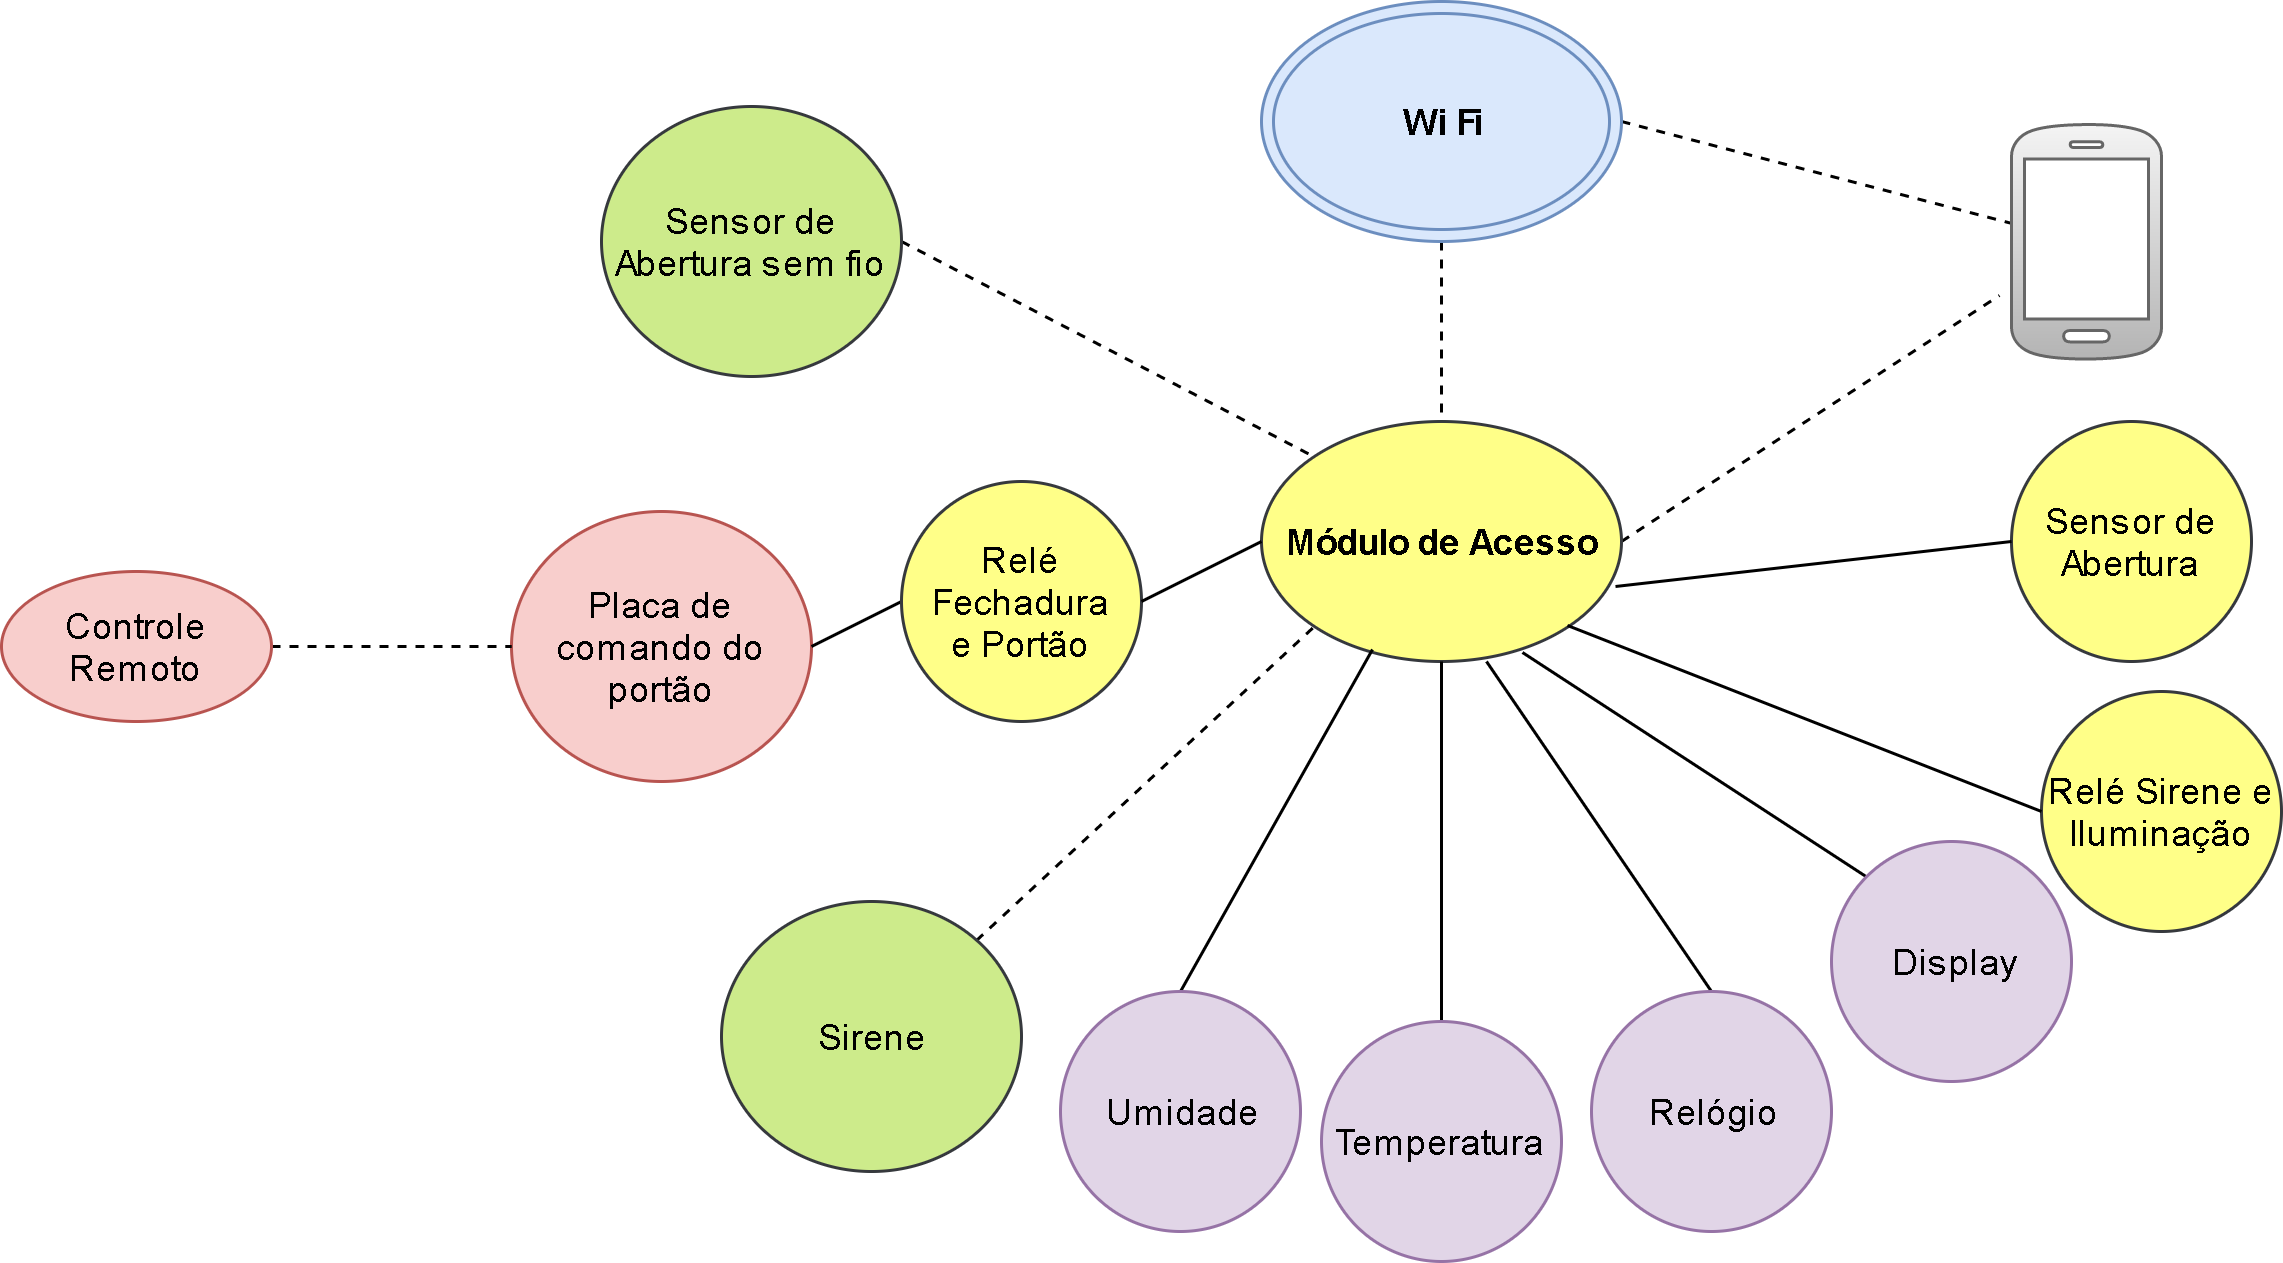
\includegraphics[width=0.8\textwidth]{diagramaModuloAcesso}
\label{fig:diagramaModuloAcesso}
\end{figure}

O diagrama ilustra o sistema já existente (em vermelho), sensor e sirene sem fio adicionais em verde (dispositivos externos ao módulo, que se comunicam por rádio), o próprio módulo de acesso, com um buzzer embutido, e sua conexão com a rede local Wi-Fi ou sua conexão direta com o celular (quando o módulo opera como um ponto de acesso de rede) em amarelo, além de funcionalidades adicionais em roxo.

A comodidade está em abrir o portão por meio do celular, por um aplicativo ou página web local, sem a necessidade de carregar uma chave ou controle. Além disso, pode prover maior praticidade (enquanto o celular está com o usuário na maioria do tempo, chave e controle podem estar na mochila). Para usuários que fazem passeios a pé, em sua maioria curtos, ou que vão à academia perto de suas casas, carregar chaves/controles é particularmente incômodo.

Por outro lado, é desejável realizar esse controle de forma segura. Por isso, o acesso é apenas local (o usuário deve estar com o celular conectado à rede local para acessar a página local, por exemplo), e um algoritmo de rotação de teclas é realizado, para evitar que pessoas mal intencionadas possam (1) olhar e copiar a senha que o usuário digita em seu celular e (2) copiar os dados de abertura e usá-los mais tarde (“middle man”). Na última alternativa, a cada acesso de um usuário, um novo mapeamento de teclas é gerado e enviado ao usuário. Mesmo que haja cópia, ela não funcionará devido ao mapeamento ter mudado. Observe ainda que a fechadura eletrônica por si só já estava vulnerável a isso (há inclusive dispositivos copiadores de senhas).

Outro aspecto de segurança é a preocupação dos usuários com o estado do portão. Muitas vezes, pode haver esquecimento ou falha e o portão ficar aberto. Para mitigar esse perigo, o módulo deve monitorar, por meio de um sensor, o estado da porta (aberto/fechado), e alertar localmente (por meio de “buzzer”) e remotamente (por email ou notificação no \textit{smartphone}, por exemplo) o usuário a abertura em horários . Essa e outras configurações (como de rede) são acessadas por meio de uma senha diferente daquela de abertura, para que a interface básica seja simples para uso.

Para o caso de falha de envio de email (servidor falha, ou algum outro problema), há um algoritmo de novas tentativas com tempos progressivamente maiores conforme as falhas ocorrerem, que busca deixar o módulo disponível para outras funções enquanto o serviço de e-mail não está disponível. No caso de indisponibilidade da internet, temos um procedimento análogo.

Para o caso de falta de conexão à internet, o módulo não seria controlável pela API, e as atualizações de dados como estado do portão seriam armazenadas para serem enviadas ao servidor em momento posterior, quando houvesse conexão à internet novamente. Caso o usuário esteja conectado à mesma rede local que o módulo, o mesmo continuaria funcionando normalmente.

Já no caso de falha da rede local, ou desconexão do módulo da rede local por problema de autenticação ou outros, o módulo de acesso ativa o \textit{Access Point}, e possibilita ao usuário acessar a rede do módulo e abrir o portão.

% TODO (victor) checar esse parágrafo abaixo. Acho que não ficou claro o que é esse "travamento"
Para evitar o travamento, um sinal de “keep alive” é monitorado, e um circuito anti travamento deve ativar um “hard reset” (reset por hardware), ou então uma rotina de “soft reset” deve ser acionada. No entanto, observe que a segunda alternativa é a mais fácil de implementar, mas a menos robusta, já que ainda pode não funcionar em casos de loop infinito.

% TODO (victor) não entendi a parte do "executa algoritmo análogo ao do envio de emails"
Outra situação que poderia gerar indisponibilidade do sistema é um ataque de DoS local (“Evil Twin”), no qual uma rede mal intencionada usa o mesmo SSID (\textit{Service Set Identifier}, o nome associado à rede WLAN) da rede original, tentando obter a senha na ocasião de reconexão de módulos. Muitas vezes, é também acompanhado de rádio interferência e outros procedimentos para fazer os módulos se desconectarem. Para mitigar o risco, cada módulo tenta inicialmente se conectar usando uma senha falsa no SSID fornecido. Caso obtenha sucesso (se a rede for aberta, como é o caso na maioria desses ataques), ele executa algoritmo análogo ao envio de emails (observe que enquanto não está conectado à rede o módulo atua como ponto de acesso e disponibiliza funcionalidades básicas). Caso ele não obtenha sucesso usando a senha errada (portanto, não detectou a situação de “evil twin”), o módulo envia a senha correta. Para proteger a rede, um controlador local do sistema pode atuar junto ao roteador e desligar a conexão sem fio enquanto a situação se manter.

O controle de acesso pode ser implementado por meio de persistência de dados de login e senha, e o uso de diversas senhas para uma residência (uma para cada morador - isso torna possível o conhecimento dos usuários que abriram o portão sem a necessidade de login prévio, facilitando o uso). O log destes acessos pode ser analisado (utilizando técnicas de Machine Learning) para determinar perfis de acesso, e evoluir até o sistema saber quando houver um acesso em horário inesperado e notificar o usuário remotamente. O aprendizado de máquina é fundamental aqui para descobrir comportamentos que podem ser entendidos como suspeitos. Para um usuário que costuma chegar em um horário aproximado todos os dias, e acionar funções semelhantes da casa, uma tentativa de acesso que não se enquadre em tais padrões pode ser produto de atividade criminosa, a qual pode ser informada pela casa para uma central, que acionará a polícia caso não seja um falso positivo.

\chapter{Projetos relacionados}

\section{Sistemas existentes no mercado}

\subsection{Sistemas comerciais}
Atualmente, já existem sistemas comerciais de automação residencial --- a maioria deles atuando de maneira mais forte do mercado norte-americano. Alguns dos sistemas mais populares nessa linha são o Amazon Echo e o Google Home.

O Amazon Echo\footnote{http://www.amazon.com/oc/echo/} consiste em um \textit{smart speaker} (alto-falante inteligente) conectado ao assistente pessoal Alexa, também da Amazon, que é capaz de entender comandos de voz. Inicialmente, funcionava como uma maneira de encomendar produtos, mas, atualmente, além de ser assistente pessoal, também é capaz de controlar diversos \textit{smart devices} da casa, como um \textit{hub} de automação residencial. Uma limitação deste produto é dependência de conexão \textit{wireless} de Internet, não sendo capaz de operar em nenhum nível sem ela.

Uma característica interessante do Alexa é a possibilidade de adição de novas \textit{skills} (habilidades) por desenvolvedores, que possuem acesso a uma API pública, documentada e disponibilizada \textit{online}. Dessa forma, seu \textit{skillset} é passível de grande expansão e personalização. Além disso, o serviço de voz desse sistema, conhecido como Alexa Voice Service, pode ser utilizado por qualquer dispositivo que contenha microfone e alto falante, e que consiga conectar-se a ele pela Internet.

O Google Home\footnote{https://madeby.google.com/home/} é similar ao Amazon Echo em alguns aspectos, sendo também um \textit{smart speaker}, que surgiu como expansão do aplicativo para smartphones Google Now, um assistente pessoal. Atualmente existe também como aplicativo para smartphones. Não é possível o desenvolvimento de módulos e expansões ao Google Home por desenvolvedores desvinculados à Google, porém ela trabalha diretamente com outras marcas e produtos para o estabelecimento de parcerias, de forma que o Google Home também consiga funcionar como \textit{hub} de automação residencial.

\subsection{Sistemas \emph{open-source}}
Também existem diversos projetos \emph{open-source} sobre o tema, cujas documentações estão disponíveis publicamente na Internet. Alguns desses projetos, analisados para o desenvolvimento do Hedwig, foram o OpenHAB e o Home Assistant.

O OpenHAB\footnote{http://www.openhab.org/} possui como objetivo principal o estabelecimento de uma plataforma de integração, capaz de solucionar o problema atual de haver diversos dispositivos em uma residência que não são capazes de se comunicar, devido à falta de uma linguagem comum para a troca informações. Por ser independente de hardware específico, é extremamente flexível e personalizável, porém isso implica em maior complexidade para o usuário no momento de sua instalação. O OpenHAB apresenta interface para o usuário em cliente web e aplicativos nativos para iOS e Android.

O Home Assistant\footnote{https://github.com/home-assistant/home-assistant} é uma plataforma de automação residencial capaz de controlar e monitorar os diversos dispositivos em uma casa, oferecendo uma plataforma web para o controle do sistema pelo usuário. O controlador local é implementado em Python, e recomenda-se instalá-lo em um Raspberry Pi. Possui diversas integrações já estabelecidas, com sistemas e serviços como o próprio Amazon Echo, Google Cast, IFTTT, Digital Ocean, entre outros, mas possibilita também a criação de novos componentes pelos próprios usuários. A personalização pelos usuários é feita por meio de um arquivo de configuração no formato YAML.

Os dois projetos apresentam como maior dificuldade a necessidade do usuário possuir conhecimentos técnicos para utilizá-los.

\section{Projeto HomeSky}

O Projeto HomeSky \cite{homeSky} é um Trabalho de Conclusão de Curso desenvolvido por alunos de Engenharia de Computação na Escola Politécnica da Universidade de São Paulo. Com o objetivo de fomentar iniciativas de desenvolvimento na área de casas inteligentes, o trabalho focou-se na criação do Rainfall, um protocolo em código aberto a nível de aplicação para ser usado na coordenação de uma rede de sensores. Isso permitiria aos desenvolvedores ter uma maior flexibilidade em seus projetos, visto que muitas das soluções existentes são proprietárias. Por fim, também foi realizada a implementação de um algoritmo de aprendizado de máquina capaz de controlar a iluminação.

\begin{figure}[H]
	\centering
	\caption{Camadas da arquitetura usada no Projeto HomeSky. As camadas em verde correspondem às bibliotecas desenvolvidas no trabalho.}
  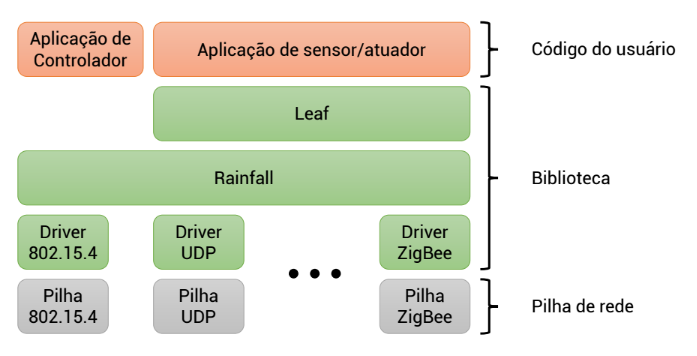
\includegraphics[width=0.8\textwidth]{arquiteturaHomeSky}
	\caption*{Fonte: \cite{homeSky}}
\label{fig:arquiteturaHomeSky}
\end{figure}

No desenvolvimento do protocolo Rainfall, foram consideradas algumas hipóteses simplificadoras a respeito da conectividade e da segurança. O protocolo não trata de forma especial a fase de conexão à rede, considerando que todos os nós já estão conectados a ela, e também considera que todos os protocolos adjacentes são confiáveis, delegando as implementações de mecanismos de reconhecimento de entrega e retransmissão ao desenvolvedor. Quanto à segurança, assume-se que a infraestrutura seja segura e que nenhum nó conectado à rede tenha comportamento mal intencionado, como por exemplo espionar mensagens destinadas a outros nós ou fingir ser o controlador.

\chapter{Especificação}

\section{Partes interessadas}
Um dos passos iniciais na elaboração de um projeto é a determinação das partes interessadas (\emph{stakeholders}). Com esse conhecimento, pode-se entender as necessidades dos diferentes perfis de clientes e as expectativas desses grupos em relação ao uso do produto. Por meio da análise de aplicação, tanto do projeto desenvolvido quanto dos dispositivos existentes, pode-se destacar os seguintes grupos dentre os potenciais consumidores:

\begin{itemize}
\item Pessoas que moram sozinhas e seus familiares;
\item Pessoas que buscam comodidade no uso e controle de dispositivos domésticos;
\item Pessoas preocupadas com o consumo de água e energia elétrica.
\end{itemize}

Considerando o Censo de 2010 \cite{ibge}, pode-se estimar as classes de consumidores para a cidade de São Paulo:

\begin{itemize}
\item Considerando que 1/10 da população com mais de 60 anos more sozinha e que 1/4 deles adquiriria o produto, temos uma estimativa de 33 mil consumidores. Como essa população está envelhecendo em taxas cada vez maiores (8,96\% em 2000 contra 13,6\% em 2016) \cite{bibliotecaVirtual}, a tendência é que essa classe aumente;
\item Considerando que 1/100 dos domicílios ocupados tenha uma pessoa com esse perfil, temos uma estimativa de 35 mil consumidores em potencial;
\item Considerando que cerca de 70\% das residências reduziram o consumo com campanhas de redução de uso de água em 2015 \cite{g1}, supondo que 5\% ficariam preocupados/interessados ao nível de se tornarem consumidores, temos uma estimativa de 71 mil consumidores em potencial.
\end{itemize}

\section{Requisitos \label{sec:requisitos}}

O levantamento de requisitos funcionais e não funcionais são definidos a seguir. Para requisitos funcionais, utilizou-se o termo \emph{RF} seguido de um número identificador --- e.g. \emph{RF-1}. Os requisitos não-funcionais levam o termo \emph{RNF}, também seguido de um identificador numérico --- e.g. \emph{RNF-1}.

\subsection{Requisitos funcionais}
\begin{description}
\item[RF-1:]O sistema deve permitir o monitoramento de aparelhos do dia a dia, dentro de uma residência, de maneira independente;
\item[RF-2:]O sistema deve ser capaz de noficar o usuário sobre o estado da casa --- e.g. temperatura, presença, etc;
\item[RF-3:]O sistema deve poder ser personalizável pelo usuário, o qual pode adicionar ou remover funcionalidades;
\item[RF-4:]O sistema deve permitir o acionamento de dispositivos da residência;
\item[RF-5:]O sistema deve ser capaz de aprender a respeito de cada usuário, podendo detectar padrões no seu comportamento e, a partir disso, sugerir ações a serem tomadas automaticamente --- e.g. acendimento automátio de lâmpadas;
\item[RF-6:]O sistema deve permitir o cadastro, remoção e atualização de usuários;
\item[RF-7:]O sistema deve permitir o cadastro, remoção e atualização de casas, para cada usuário;
\item[RF-8:]O sistema deve permitir o cadastro, remoção e atualização de dispositivos, para cada casa;
\item[RF-9:]O sistema deve permitir o seu reinício (\emph{reset});
\item[RF-10:]O sistema deve permitir a autenticação de usuários;
\item[RF-11:]O sistema deve permitir a configuração de dispositivos;
\item[RF-12:]O sistema deve disponibilizar uma \emph{API} para comunicação.

\end{description}

\subsection{Requisitos não-funcionais}
O levantamento de requisitos não-funcionais foi realizado com base na norma ISO25010:2011 \cite{iso25010}.

\begin{description}
\item[RNF-1:]Os dispositivos que compõem o sistema dentro de uma residência devem ser independentes entre si, devendo obedecer a uma interface comum de integração com o \emph{core} do projeto, para que seja facilitada a sua ampliação e extensão, com outras funcionalidades;
\item[RNF-2:]O sistema deve garantir segurança dos dados por meio de protocolos de comunicação seguros. O tráfego de informação entre as residências e os servidores externos não pode ser realizado em texto aberto. A comunicação interna da casa deve ser realizada em canais restritos;
\item[RNF-3:]Os dados de cadastro do sistema devem ser armazenados em servidores seguros \cite{softwareSecurity};
\item[RNF-4:]O sistema deve ser robusto, de modo a continuar operando, mesmo com menor nível de funcionalidades, quando há ocorrência de falhas na comunicação entre a casa e serviços externos --- e.g. indisponibilidade parcial devido a problemas com servidores remotos, indisponibilidade total devido a perda da conexão com a Internet --- ou falhas na rede interna, como a indisponibilidade de conexão local. A validação é realizada com interrupções na rede, desconexão e desligamentos de servidores e dispositivos, seguida da verificação dos serviços disponíveis;
\item[RNF-5:]O sistema deve identificar e se recuperar de travamentos em suas partes, reiniciando-as;
\item[RNF-6:]O sistema deve possuir mecanismos de proteção contra ataques de negação de serviço (\emph{DoS});
\item[RNF-7:]O sistema deve apresentar disponibilidade de 99,9\% --- cerca de 8 horas de indisponibilidade por ano. Essa medida de disponbilidade refere-se somente aos serviços remotos, não levando em consideração indisponibilidades das residências;
\item[RNF-8:]O sistema deve ser escalável a até 10 mil usuários, sem perdas de desempenho consideráveis, ou aumento na latência para as requisições serem atendidas, com variação de até 5\%. A verificação deve ser realizadas com softwares de análise de performance comerciais\footnote{Um exemplo de aplicação de monitoramento de rede é desenvolvida pela empresa Dynatrace \url{https://www.dynatrace.com/} };
\item[RNF-9:]O sistema deve possuir instalação intuitiva e simplificada --- a instalação é realizada em passos, seguindo o manual de instruções, sem a necessidade de conhecimentos de computação ou eletrônica;
\item[RNF-10:]O sistema deve atender e processar requisições em paralelo, tanto dos usuários quanto dos dispositivos físicos;
\item[RNF-11:]O sistema deve autenticar e autorizar as requisições recebidas, descartando as requisições inválidas.
\end{description}

\subsection{Funcionalidades por nível de conectividade}

Os requisitos apresentados anteriormente detalham o sistema completo. Para que o requisito \emph{RNF-4} fosse implementado, o projeto incorporou três níveis de funcionalidade --- \emph{Online}, \emph{Local} e \emph{Offline}. O primeiro nível, \emph{Online}, é o mais amplo e caracteriza o comportamento normal do sistema, quando todas as conexões estão disponíveis, e os dispositivos e serviços funcionam corretamente. O nível \emph{Local} modela o cenário de não haver possibilidade de conexão externa com a casa, como é o caso quando não há internet disponível. O último nível, \emph{Offline}, reflete uma situação emergencial, no caso de problemas com o servidor interno, por exemplo.

\chapter{Arquitetura}
% TODO rever tudo nesse arquivo

\section{Visão geral}

\section{Evolução arquitetural}
O processo de escolha para a arquitetura utilizada foi iterativo, e foram analisados os pontos fracos e as vantagens de cada nova sugestão.

A primeira versão proposta baseava-se unicamente em microsserviços, responsáveis por toda a inteligência do projeto, o que a fazia interessante do ponto de vista da escalabilidade, para um número muito grande de casas. Com uma arquitetura fundamentalmente desenvolvida assim, também é possível utilizar quantas tecnologias forem necessárias ou desejáveis para cada um dos serviços, sem efeitos colaterais nos outros, transparentemente.. Por outro lado, cria-se grande complexidade na integração entre todos os serviços disponíveis, mas que pode ser gerenciada por técnicas conhecidas, e também explicadas aqui (como a coreografia e a orquestração). O overhead para a comunicação, no entanto, é aumentado, e os serviços necessitam de um meio rápido e robusto, que implemente qualidade de serviço para padrões diferentes de mensagens. Foi proposto um gateway para os serviços da nuvem, onde passaria toda a comunicação com a casa. A inserção do gateway, no entanto, cria um ponto único de falha.

\begin{figure}[H]
	\centering
	\caption{Primeira versão da arquitetura do projeto Hedwig}
  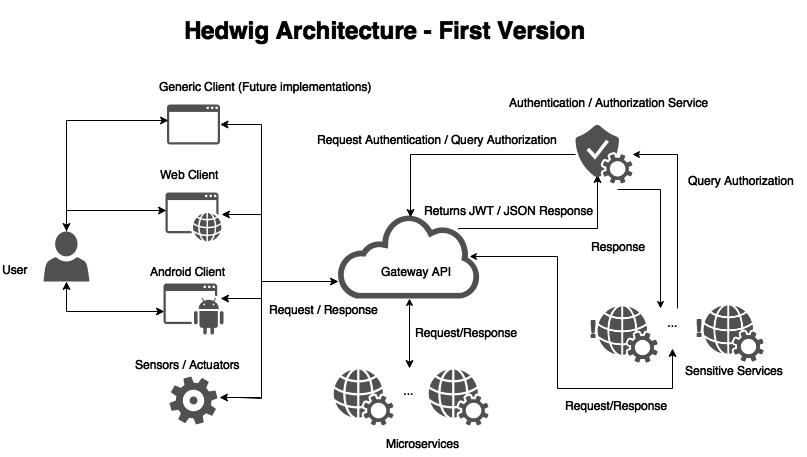
\includegraphics[width=0.8\textwidth]{arquiteturaV1}
\label{fig:arquiteturaV1}
\end{figure}

É possível observar que alguns microsserviços são classificados como sensitivos, os quais dependem de nova consulta ao serviço de autenticação e  autorização, para garantir a segurança. Esses serviços são todos aqueles responsáveis por tomar uma ação em relação à casa que envolva riscos. Os microsserviços não sensitivos utilizam a autenticação já realizada pelo gateway, na chegada do request.

Quando uma requisição chega à nuvem, ela deve ser autenticada, e caso passe nos critérios de autenticação e autorização, é retornado um JWT (JSON Web Token), necessário para os passos seguintes. O token JWT é discutido aqui, na seção MARCAR SEÇÃO AQUI.

De extrema importância, e não cobertos pela arquitetura anterior, são os requisitos de disponibilidade do projeto. Se o gateway estiver inacessível em determinado momento, a casa não terá mais nenhuma forma de comunicação com os meios externos, mesmo para os serviços mais básicos. Para resolver este problema, foi proposta uma segunda versão, conforme ilustra a imagem seguinte.

\begin{figure}[H]
	\centering
	\caption{Segunda versão da arquitetura do projeto Hedwig}
  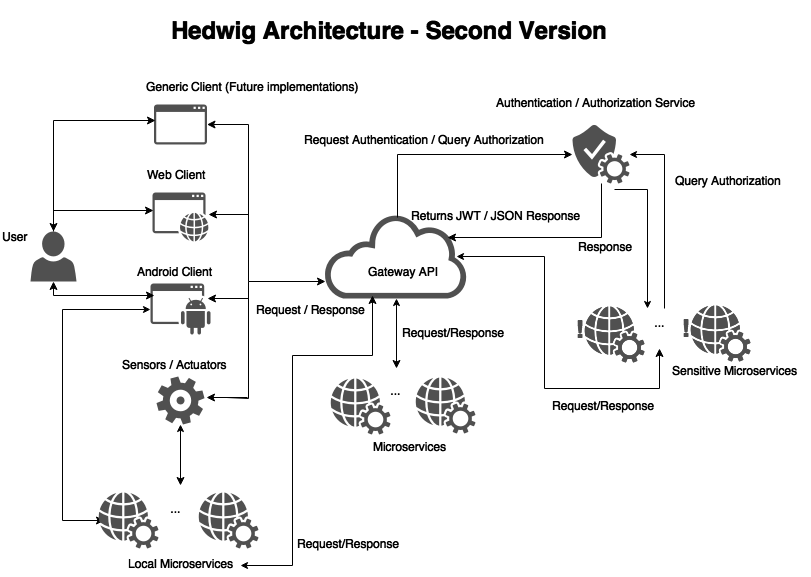
\includegraphics[width=0.8\textwidth]{arquiteturaV2}
\label{fig:arquiteturaV2}
\end{figure}

Nesta versão, serviços essenciais seriam duplicados dentro da casa, e no caso de haver qualquer forma de impedimento na comunicação com a nuvem, esses serviços seriam responsáveis por controlar diretamente os atuadores desejados. Entretanto, cria-se mais uma complexidade, ao manter serviços duplicados na casa, e no caso destes serviços não estarem online no momento necessário, também não seriam alcançados requisitos mais fortes de disponibilidade. Contudo, é uma versão que chega mais próximo de obedecer às necessidades do projeto.

Essa arquitetura provê módulos sem inteligência, e todo o controle é feito pelo serviço correspondente. Ao mesmo tempo que essa escolha tem benefícios, como a escalabilidade, a manutenção (já que é muito mais simples atualizar o software de um ponto único, sempre que necessário), para correções ou possíveis aumentos de funcionalidade. Porém, não ficaríamos livres, mais uma vez, do ponto único de falha. Também, alguns módulos ficariam em lugares de difícil acesso, ou mesmo fora da casa, onde a comunicação poderia ser perdida, ou ser intermitente. Assim, em caso de falha de comunicação, um atuador não receberia os sinais necessários do serviço, acarretando em sérios problemas de segurança. No caso de uma garagem, por exemplo, o portão permaneceria aberto indeterminadamente, ou poderia não ser aberto o morador chegasse em csa.

Assim, começamos o desenvolvimento de um modelo arquitetural modularizado, onde cada módulo teria inteligência para realizar as tarefas necessárias e, ao mesmo tempo, podendo enviar dados à nuvem, e ser avisado quando deve realizar uma tarefa. Com isso, em um aspecto também comercial, módulos inteiros poderiam ser vendidos, substituídos e aumentados.

A arquitetura escolhida, também faz uso de microsserviços, no lado da nuvem, e no lado da casa os componentes de hardware passam a ser agrupados em módulos independentes, com responsabilidades bem estabelecidas, inteligência para fazer todas as atividades necessárias, e com comunicação a um servidor local, que realizará, por último, a comunicação direta com os serviços não locais. Esse servidor se comunicaria com módulos por meio de mensagens, enviadas em tópicos, as quais seriam interpretadas e enviadas aos servidores remotos. Se a casa perder comunicação com a nuvem, o servidor local armazenará as mensagens, que serão enviadas posteriormente. Essas mensagens, no caso, seriam de dados, advindas de sensores em módulos. Como não há urgência para o processamento de tais dados, os quais serão utilizados para análise de comportamento e machine learning, não há prejuízo com o eventual envio tardio.

Quando a comunicação entre o servidor local e a nuvem for perdida, os aplicativos web ou mobile, poderão se comunicar diretamente com o servidor local da casa, para acessar uma quantidade mais restrita e essencial de ações (como liberação de acesso, por exemplo). Além disso, no caso de perda de comunicação com o servidor local também, os aplicativos poderão se comunicar diretamente com os módulos para terem acesso aos serviços de extrema importância.

Por ser escolhida, essa arquitetura será extensivamente detalhada e discutida aqui, com seus benefícios e limitações.

\section{Módulos}
Para a criação dos módulos de hardware, foram escolhidos componentes de IoT comerciais, que possuem preços acessíveis, ampla documentação disponível e uma comunidade de desenvolvedores crescente.

A interconexão dos componentes, bem como a comunicação com o mundo externo pela internet será intermediada por um servidor local, que rodará na plataforma Raspberry Pi, rodando um sistema operacional Linux (Raspbian), baseado em Debian, e que dispõe da interface de hardware necessária para conexão com a rede.

Os sensores e atuadores devem ser conectados fisicamente com um módulo controlador, de modo que, para contornarmos essa limitação, utilizaremos módulos ESP8266 para transmissão sem fio por meio do WiFi. Esses módulos serão responsáveis pela transmissão das informações recebidas para o servidor local. Toda a arquitetura para essa transmissão será detalhada mais à frente. Os outros módulos a serem utilizados, como sensores DHT11, LM555, etc,  podem ser vistos no anexo, em uma lista completa. % TODO precisa colocar essa lista no anexo

Em geral, esses módulos consistem do microcontrolador, relés, sensores e fontes/conversores de tensão a depender do módulo, além de um circuito para manutenção corretiva baseado no astável 555, conectados à rede WiFi e/ou trabalhando como pontos de acesso. Para casos de falha de conexão, há um algoritmo de novas tentativas com tempos progressivamente maiores conforme as falhas ocorrerem, que busca deixar o módulo disponível para outras funções enquanto o serviço não está disponível. Para evitar o travamento, um sinal de “keep alive” é monitorado, e um circuito anti travamento deve ativar um “hard reset” (reset por hardware), ou então uma rotina de “soft reset” deve ser acionada. No entanto, observe que a segunda alternativa é a mais fácil de implementar, mas a menos robusta, já que ainda pode não funcionar em casos de loop infinito.

\subsection{Módulos Base}
\subsubsection{ESP8266}
O ESP8266 é um microprocessador com baixo consumo e conexão WiFi 802.11 integrada \cite{espressif}. Pode ser programado usando a Arduino IDE, já muito utilizada \cite{thomsen}. Opera com uma tensão de 3.3 V, suporta WPA e possui modo de interrupção somente por software. É amplamente usado como shield para conexão WiFi de placas de desenvolvimento da plataforma Arduino; contudo, no projeto Hedwig, o utilizaremos em modo StandAlone como principal processador e responsável pela conexão dos diferentes módulos de automação. Suas duas principais plataformas de desenvolvimento são Wemos\footnote{Plataforma Wemos: https://www.wemos.cc/} e NodeMCU\footnote{Plataforma NodeMCU: http://nodemcu.com/}. O projeto utilizará o Wemos D1 Mini, versão compacta da Wemos D1 R2.

Possui um modo de operação de baixa potência (sleep mode), em que o nível de funcionalidades fica limitado, contudo o consumo de bateria fica muito menor. Podemos usar 7 portas de E/S digitais e uma porta de entrada analógica. Duas portas são inutilizáveis, pois são usadas para programação e outras tarefas do sistema integrado do ESP8266. Uma alternativa para extensão de portas é utilizar, por exemplo, três níveis de sinal análogico para detectar três tipos de acionamento (através de um circuito dedicado, com priorização de entrada), interface I2C (como o usado para o display) e uso de Radio Frequência, através de um par receptor-transmissor integrado no módulo, controles, atuadores e sensores sem fio.

% TODO tirar esse paragrafo abaixo daqui e coloca-lo em uma secao sobre o modulo de acesso a casa
Dentre os materiais adquiridos, destacam-se como exemplos o controle RF  e sensor de abertura de portão sem fio - observe que a fechadura eletrônica já existe na residência teste, logo é utilizada nesse projeto, contudo não está na lista de materiais para aquisição.

\subsubsection{Multiplexação no tempo}
Para tratar indisponibilidade dos módulos devido a tentativas de reconexão e conexão e requisições não gerenciadas e aumentar a disponibilidade, além do circuito antitravamento e hard reset, as diversas rotinas (desde configuração inicial, reconfigurações, coletas de dados, atuar por meio de relés, até conexão, desconexão, reconexão e envio de dados) foram multiplexadas no tempo da seguinte forma:

\begin{figure}[H]
	\centering
	\caption{Rotina de multiplexação de procedimentos no tempo}
  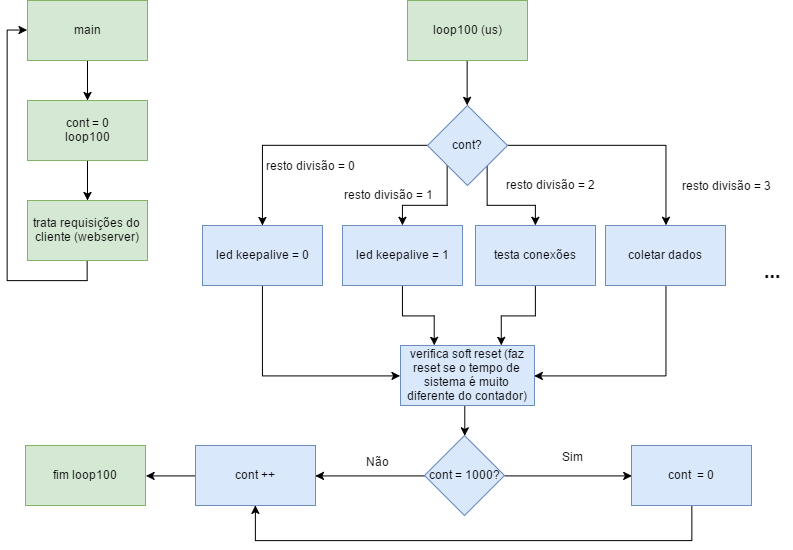
\includegraphics[width=0.8\textwidth]{rotinaMultiplexacao}
\label{fig:rotinaMultiplexacao}
\end{figure}

\subsubsection{Tratamento de indisponibilidade}
Nos casos de indisponibilidade de internet, servidor ou rede local, o seguinte procedimento foi adotado: (observe que a indisponibilidade do próprio módulo é tratada pelo circuito antitravamento).

\begin{figure}[H]
	\centering
	\caption{Tratamento de indisponibilidade de recursos}
  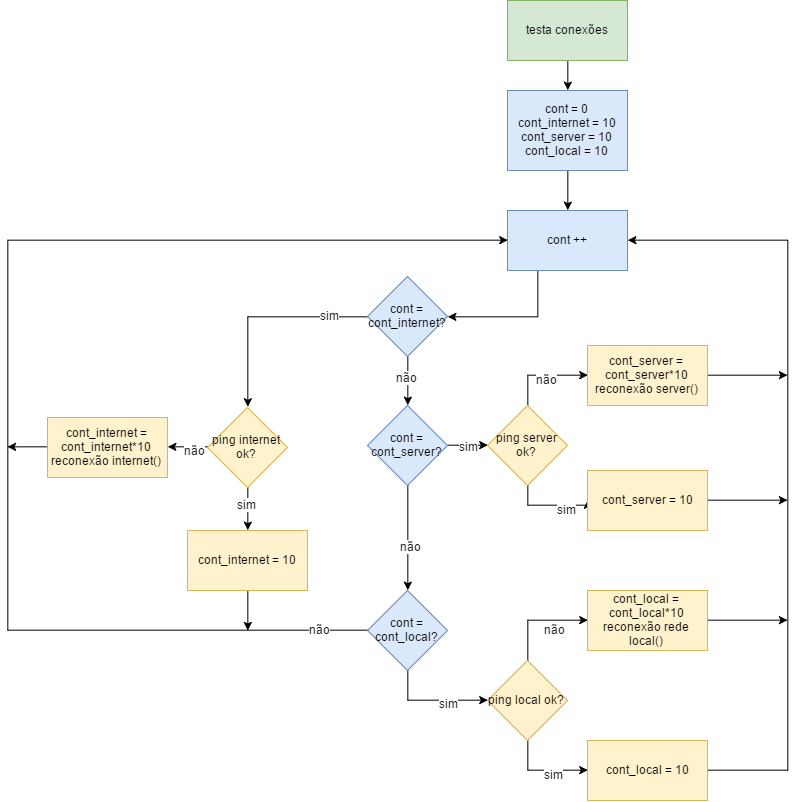
\includegraphics[width=0.8\textwidth]{tratamentoIndisponibilidade}
\label{fig:tratamentoIndisponibilidade}
\end{figure}

Com esse procedimento, as tentativas de reconexão à internet, servidor e rede local estão segregadas e com tentativas realizadas em intervalos de tempo sucessivamente maiores. Desta forma, conseguimos gerenciar esses procedimentos, já que o nível de processamento é baixo.

\subsubsection{DoS Local (Evil Twin)}
No caso de ataque de Evil Twin, no qual uma rede mal intencionada, usualmente aberta, usa o mesmo ssid da rede original, com o objetivo de obter a senha, o sistema pode ficar indisponível até ao nível local. Módulos podem se conectar à rede mal intencionada e ficarem somente com as funcionalidades offline (como acionamento de lâmpada por botão física acoplado ao módulo). Outro problema é a queda da rede por interferência de radio frequência ou outro mecanismo utilizado pelo usuário mal intencionado para que os clientes se desconectem, tentem reconexão e forneçam a senha da rede.

Para mitigar esses riscos, os módulos executam o seguinte procedimento:
\begin{figure}[H]
	\centering
	\caption{Tratamento de ataque de DoS Local}
  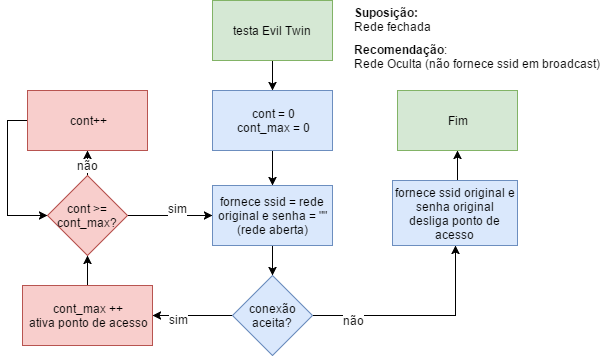
\includegraphics[width=0.8\textwidth]{tratamentoDoS}
\label{fig:tratamentoDoS}
\end{figure}

\subsubsection{Diagrama}
Segue diagrama do circuito impresso (PCB) feito em conjunto com o Projeto Katz-House\footnote{Katz-House, Fabio Hayashi. Projeto Pessoal, 2017.}. Funcionalidade, componentes e arquitetura foram responsabilidade do Projeto Hedwig, enquanto a disposição física, se atentando para problemas de interferência e mantendo um módulo menor possível foi responsabilidade do Projeto Katz-House.

\begin{figure}[H]
	\centering
	\caption{Diagrama PCB do Módulo Base}
  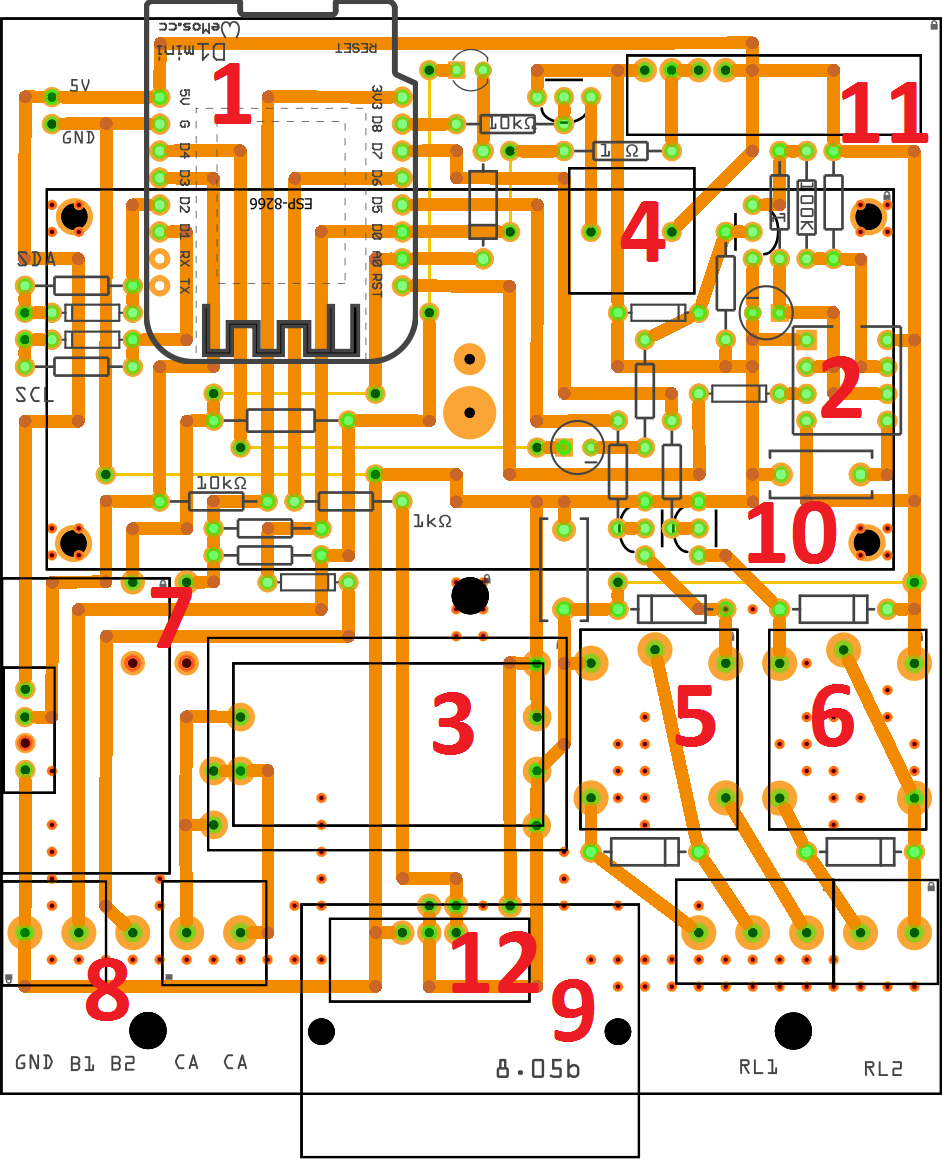
\includegraphics[width=0.8\textwidth]{diagramaModuloBase}
\label{fig:diagramaModuloBase}
\end{figure}

\begin{enumerate}
\item Wemos D1 mini
\item Astável 555
\item Fonte 5V 3W
\item Buzzer
\item Relé 1
\item Relé 2
\item Hard Reset
\item Botões
\item Presença
\item RF-RX
\item RF-TX
\end{enumerate}

\begin{figure}[H]
	\centering
	\caption{Diagrama PCB do Módulo Base}
  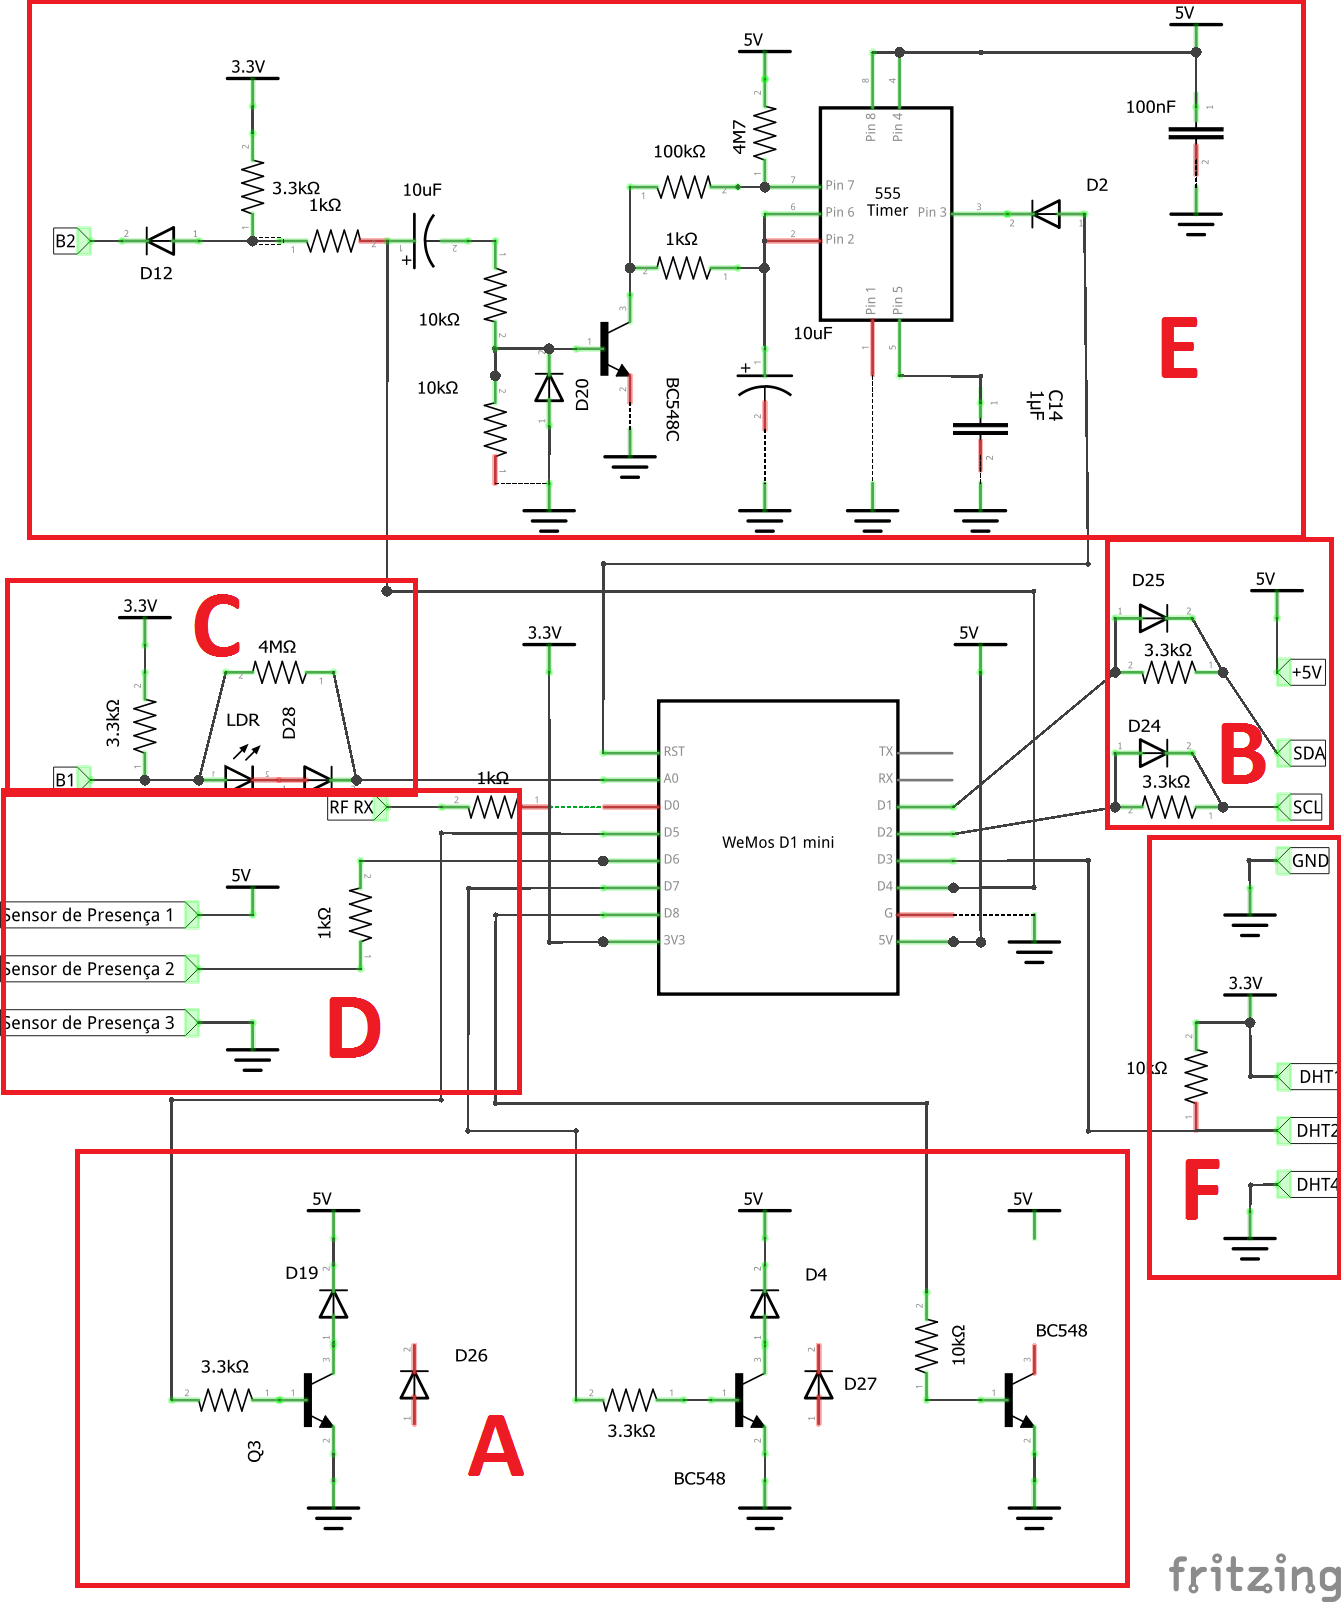
\includegraphics[width=0.8\textwidth]{esquematicoModuloBase}
\label{fig:esquematicoModuloBase}
\end{figure}

\begin{description}
\item [A - Saídas] Circuitos simples de transistor para acionamento de relés (para lâmpadas) e buzzer.
\item [Proteção 3V3 5V] Como o display trabalha com tensão de 5V, há proteções com diodos para não danificar as entradas digitais do Wemos D1 mini, que trabalha com tensão de 3V3.
\item [3 Entradas em A0] O circuito tem como entradas um botão (para acionamento do relé 1), o LDR (para chaveamento do backlight do display), e um outro botão para hard reset do dispositivo, todos numa entrada analógica, cujo mapeamento E/S é da seguinte forma:

\begin{figure}[H]
	\centering
	\caption{Entradas Em A0}
  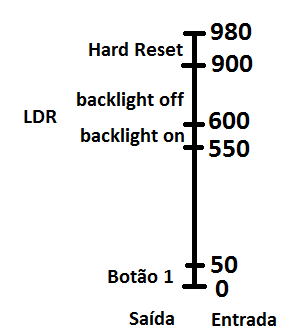
\includegraphics[width=0.4\textwidth]{entradasEmA0}
\label{fig:entradasEmA0}
\end{figure}

\item [Presença ou RF-TX] A entrada digital D6 é usada exclusivamente como entrada do sensor de presença PIR ou receptor RF.
\item [Astável 555 para Hard Reset e Botão] A porta D6 é usada como LED “keep alive” do módulo. Sua demora ao piscar indica que o módulo está travado ou demorando muito para processar algo (o que não deveria acontecer, uma vez que os procedimentos estão multiplexados no tempo, de acordo com seus tempos limite). Dessa forma, conectamos essa saída a um circuito antitravamento, que executa o reset caso nos casos mencionados, de travamento ou “timeout”.

O primeiro capacitor tem como objetivo desacoplamento DC, de forma que a entrada do circuito envolvendo o astável 555 seja somente AC. Assim, travamentos em 0 ou 1 indicam travamento.

Enquanto o led pisca em intervalos esperados (regularmente), o transistor conduz e mantém uma saída dente de serra muito próxima de 0. Quando o módulo trava, o transistor não conduz mais, e a saída passa a oscilar entre 1/3 e 2/3 da tensão total (observe que o carregamento é feito pelo resistor de 4M7, muito maior que o resistor de 100k, fazendo com que o tempo de carga seja muito maior que o tempo de descarga, uma vez que esses tempos são diretamente proporcionais à constante de tempo dos circuitos RC, que é dada pelo produto do R*C). Durante a descarga, o reset da placa é realizado. Observe que os tempos foram ajustados pelos valores dos componentes discretos, para que o tempo entre resets sucessivos seja menor que o tempo necessário para o módulo voltar a funcionar após um reset.

Segue abaixo uma ilustração sobre o funcionamento do circuito.

\begin{figure}[H]
	\centering
	\caption{Funcionamento do Circuito de Antitravamento}
  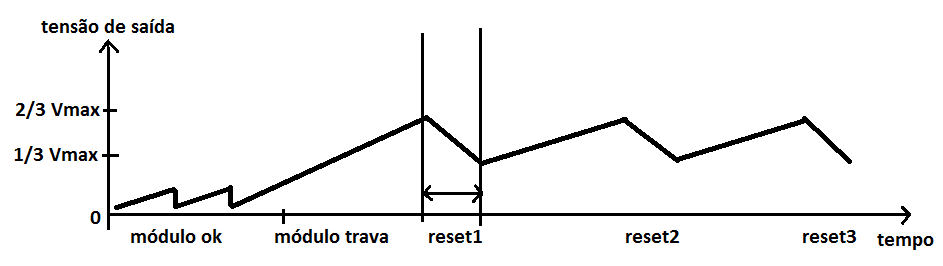
\includegraphics[width=0.8\textwidth]{circuitoAntiTravamento}
\label{fig:circuitoAntiTravamento}
\end{figure}

\item [DHT11] Entrada D3 é ligada a uma montagem básica para leitura de umidade e temperatura através do periférico DHT11.

\end{description}

\subsubsection{Montagem}

\subsection{Módulo de Interface com Sistema de Alarmes}
\subsubsection{Especificação}
\subsubsection{Montagem}

\subsection{Módulo de Acesso}
\subsubsection{Especificação}
\subsubsection{Montagem}

\subsection{Módulo de Quarto}
\subsubsection{Especificação}
\subsubsection{Montagem}

\subsection{Módulo de Aquário}
\subsubsection{Especificação}
\subsubsection{Montagem}

\subsection{Módulo de Cozinha}
\subsubsection{Especificação}
\subsubsection{Montagem}

\section{Controlador Local}
Para a intercomunicação entre os módulos e a nuvem, há a presença do servidor local Morpheus, responsável por introduzir mais uma camada de segurança, na autenticação das mensagens e garantir que as autorizações necessárias para os procedimentos existam. Para isso, foi desenvolvido um sistema de mensageria, com a definição de um protocolo de comunicação entre os serviços de nuvem e os módulos, e dos módulos para os serviços. Assim, quando um usuário desejar realizar determinada operação por meio do cliente web, uma mensagem é enviada, a qual será interpretada pelo servidor local, e em seguida encaminhada para o destino, por meio do protocolo MQTT, com o broker Mosquitto.

\subsection{Requisitos funcionais}
\begin{itemize}
\item Configuração dos módulos, de acordo com as regras e interfaces estabelecidas. Irá enviar para os módulos os novos parâmetros (vindos da nuvem) para se adaptar, de acordo com as necessidades do usuário;
\item Autenticação local do usuário;
\item Envio dos dados vindos do módulo para a nuvem, para que sejam tratados. É necessário estabelecer interface para a comunicação e formato dos dados;
\item Persistência de dados. Quando não houver conexão, o servidor deverá armazenar os dados localmente, e depois enviar para a nuvem;
\item Envio de pedidos de tomadas de ação para os módulos.
\end{itemize}

\subsection{Formato dos Tópicos MQTT}
hw\/\textless nome\_do\_modulo\textgreater	\/s2m (Server to Module - o módulo deve ser subscriber desse tópico. O servidor deve ser publisher desse tópico).

hw\/\textless nome\_do\_modulo\textgreater	\/m2s (Module to Server - o servidor deve ser subscriber desse tópico. O módulo deve ser publisher desse tópico).

\subsection{Regras de Negócio}

\begin{itemize}
\item Após a compra de cada módulo, o usuário deverá registrar online a aquisição. O servidor da nuvem enviará para o servidor local, da casa, a requisição para configurar o módulo;
\item Cada módulo enviará mensagens para o servidor local com o seus dados, por meio do MQTT. A interface de comunicação deve ser estabelecida;
\item Troca de senha do wifi: O usuário cadastra no site a nova senha. O servidor na nuvem faz a requisição para o servidor local, o qual enviará um arquivo de configuração com a nova senha para cada um dos módulos registrados. Após a configuração de todos os módulos, o servidor local envia resposta de sucesso para a nuvem, a qual indica ao usuário que a troca de senha já pode ser feita com sucesso;
\item Todo módulo sai de fábrica configurado com o tópico que deve se inscrever e publicar;
\item Cada módulo terá um certificado digital. O broker MQTT somente deixará alguém ser publisher/subscriber de um tópico caso tenha esse certificado.
\end{itemize}

\subsection{Definição de Interfaces}
\begin{itemize}
\item Dois tipos de mensagens do servidor para os módulos: Configuração (configuration) e Requisição de Ação (action\_request);
\item Três tipos de mensagens dos módulos para o servidor: Confirmação (confirmation), Envio de Dados (data\_transmission) e Data Request (data\_request).
\end{itemize}

\subsection{Definição das Mensagens}
\subsubsection{Configuração (configuration)}
\begin{itemize}
\item Sentido: Servidor para módulo
\item Protocolo: MQTT
\item Uso: Envio dos parâmetros para se adaptar ao comportamento do usuário (Machine Learning). Isso ocorre quando o algoritmo de ML, na nuvem, identifica a necessidade de modificar um comportamento do módulo. O servidor da nuvem envia uma mensagem para o servidor local, com a identificação de cada módulo e quais variáveis devem ser modificadas em cada um deles.
\item Definição do formato:
\#configuration
\$ts:\textless timestamp\textgreater
\$ty:\textless tipo da configuracao\textgreater
@
\textless dados a serem interpretados pelo módulo\textgreater
@
\end{itemize}

\subsubsection{Requisição de ação (action\_request)}
\begin{itemize}
\item Sentido: Servidor para módulo
\item Protocolo: MQTT
\item Uso: Quando um usuário faz a requisição de uma ação por meio do aplicativo. Por exemplo, quando deseja-se acender uma luz, o aplicativo envia uma requisição para o servidor local, o qual enviará uma mensagem de action\_request para o módulo correspondente.
\item Definição do formato:
\#action\_request
\$ts:\textless timestamp\textgreater
\$ty:\textless tipo da ação\textgreater
@
\textless dados a serem interpretados pelo módulo\textgreater
@
\end{itemize}

\subsubsection{Confirmação (confirmation)}
\begin{itemize}
\item Sentido: Do módulo para o servidor
\item Protocolo: MQTT
\item Uso: Confirmação de uma configuração, patch ou requisição de ação, vindas do servidor.
\item Definição do formato:
\#confirmation
\$ts:\textless timestamp\textgreater
\$ty:\textless tipo da confirmação\textgreater
@
\textless dados a serem interpretados pelo servidor\textgreater
@
\end{itemize}

\subsubsection{Transmissão de dados (data\_transmission)}
\begin{itemize}
\item Sentido: Do módulo para o servidor
\item Protocolo: MQTT
\item Uso: Envio de dados de sensores para o servidor
\item Definição do formato:
\#data\_transmission
\$ts:\textless timestamp\textgreater

\$ty:\textless tipo de dados\textgreater
@
*
sn:\textless sensor name\textgreater
vl:\textless value\textgreater
*
*
sn:\textless sensor name\textgreater
vl:\textless value\textgreater
*
*
sn:\textless sensor name\textgreater
vl:\textless value\textgreater
*
@
\end{itemize}

\subsubsection{Requisição de dados (data\_request)}
\begin{itemize}
\item Sentido: Do módulo para o servidor
\item Protocolo: MQTT
\item Uso: Requisição de alguma informação do servidor. Ex.: Atualização de hora
\item Definição do formato:
\#data\_request
\$ts:\textless timestamp\textgreater
\$ty:\textless request\_type\textgreater
\end{itemize}

\begin{figure}[H]
	\centering
\caption{Tópicos MQTT}
  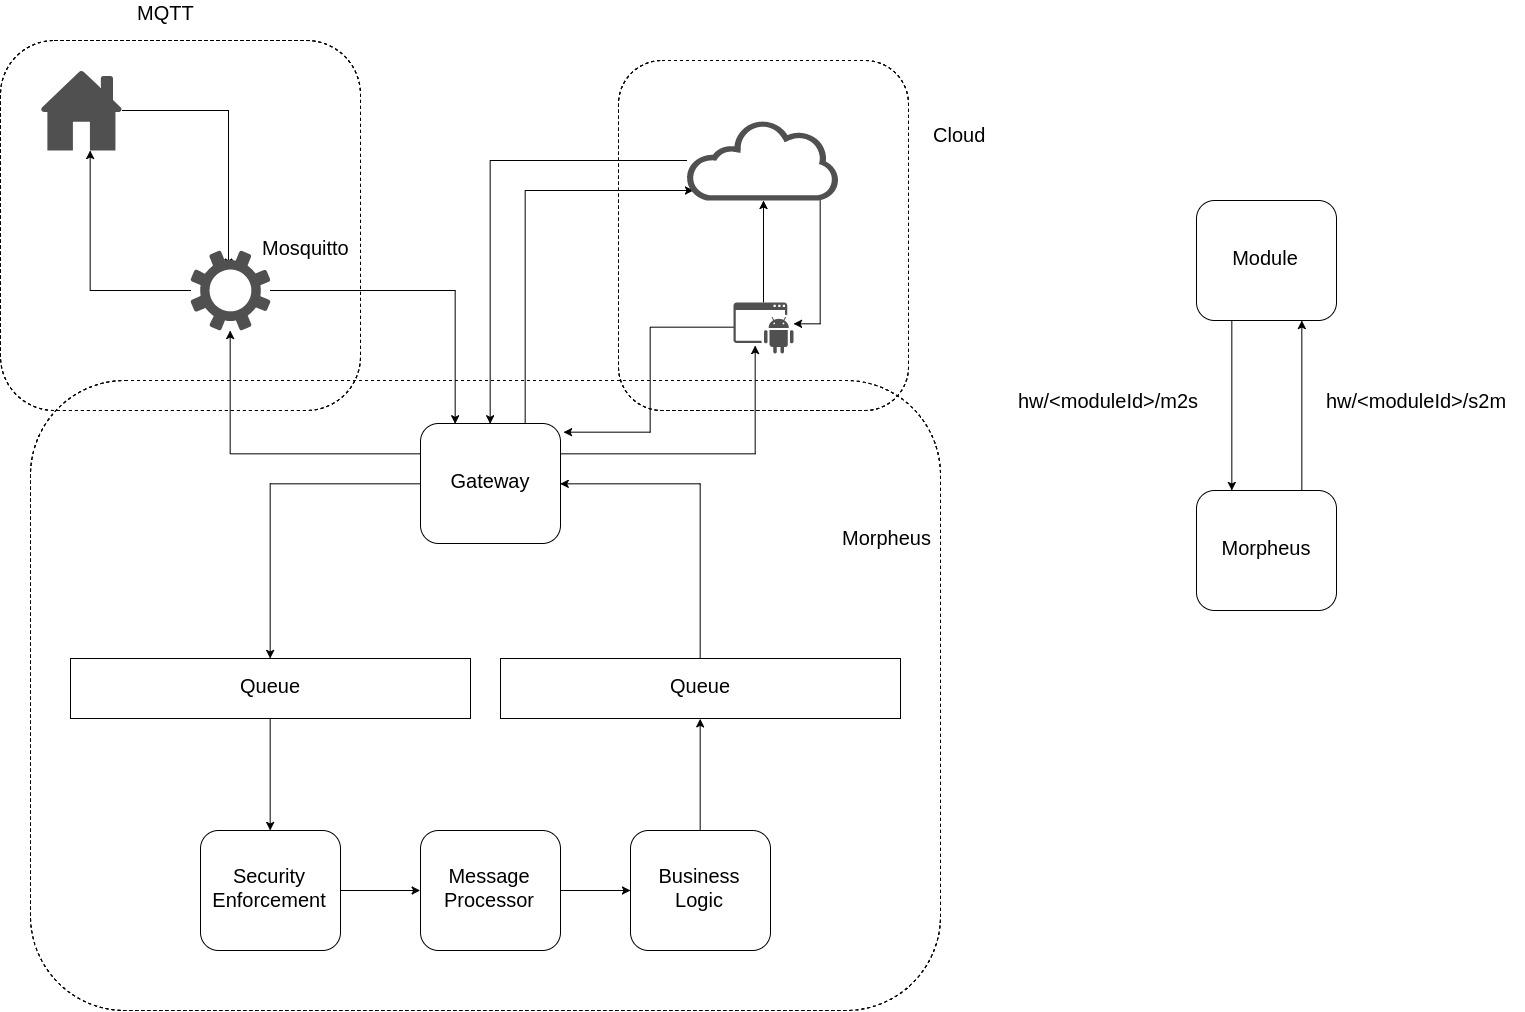
\includegraphics[width=0.8\textwidth]{topicosMQTT}
\label{fig:topicosMQTT}
\end{figure}

\subsection{Raspberry Pi}
O Raspberry Pi é um computador integrado num único chip, do tamanho de um cartão de crédito. Foi desenvolvido com o objetivo de promover o ensino de computação básica, que possui funcionalidades tais como um computador desktop: navegação na internet, reprodução de video, processamento de texto, dentre outros. No projeto, será utilizado como servidor local (gerenciador de módulos local da casa), exatamente pelas funcionalidades compatíveis com a de um computador desktop.

A versão 3 possui uma CPU 1.2 Ghz 64-bit quad-core ARMv8, conexão 802.11n Wireless LAN, Bluetooth 4.1, suporte a Bluetooth Low Energy (BLE), 1GB RAM, 4 portas USB, 40 pinos GPIO, porta HDMI, porta Ethernet, interface para câmera, display e cartão SD. Para projetos que necessitem de baixo consumo energético, os modelos mais indicados são Pi Zero ou A+ \cite{raspPi}.

\section{Servidor na Nuvem}
Como foi escolhida uma arquitetura baseada microsserviços para construção do projeto, módulos diferentes podem ser escritos em linguagens de programação diferentes, o que promove uma maior flexibilidade não só durante o desenvolvimento dos módulos de mostrados nesse trabalho, mas também daqueles projetados futuramente como extensões do sistema Hedwig.

Para o desenvolvimento dos módulos definidos na especificação do projeto, utilizamos tecnologias atuais que são utilizadas em grandes empresas de tecnologia do mundo e possuem vasta documentação, referências e fontes de conhecimento como tutoriais e exemplos.
Para o desenvolvimento da parte de software, utilizaremos tecnologias atuais, que são também utilizadas nas maiores empresas de tecnologia do mundo. De acordo com o planejamento, utilizaremos uma arquitetura de microsserviços para construção do projeto. Com esta técnica, módulos diferentes poderiam ser escritos em, inclusive, linguagens de programação diferentes, o que promove uma maior flexibilidade durante o desenvolvimento.
Para o desenvolvimento da API, responsável pelos módulos sendo executados na nuvem e comunicação com banco de dados, utilizaremos Node.js (interpretador de código JavaScript do lado do servidor), com a utilização de alguns frameworks como é o caso do Express. O banco de dados com a qual ela se conecta é do tipo MongoDB (banco de dados orientado a documentos). Tais decisões foram baseadas no fato de bancos de dados em MongoDB serem altamente escaláveis e flexíveis, assim como Node.js, que, por sua arquitetura movida a eventos de E/S que não bloqueiam o servidor, provê ao mesmo uma altíssima escalabilidade, ao permitir milhares de conexões simultâneas, sem impacto na performance do servidor. Além disso, o fato de que os dados provindos do banco já estão organizados em objetos, e dessa forma, podem ser recebidos prontamente como objetos JavaScript no código em Node.Js geram facilidade e fluidez para o desenvolvimento do código.

\subsection{Arquitetura de Microsserviços}
\subsubsection{Características}
A arquitetura de microsserviços é um estilo que compreende a estruturação de uma aplicação em um conjunto de serviços com baixo grau de acoplamento que se comunicam por meio de protocolos de comunicação leves.

Para melhor compreender essa arquitetura, podemos compará-la à arquitetura monolítica. Uma aplicação monolítica está contida em uma única unidade, que geralmente é dividida em camadas de funcionalidade tecnológica como interface web, camada de negócios server-side e camada de persistência de dados. A escalabilidade desse modelo é dada por meio do aumento do número de servidores, máquinas virtuais ou contêineres juntamente a um load balancer - é a chamada escalabilidade horizontal. Uma alteração em uma pequena parte da aplicação significa que toda a aplicação deverá passar por um processo de build e deploy. Já a arquitetura de microsserviços divide as funcionalidades em serviços autônomos, muitas vezes usando as regras de negócios para realizar essa divisão. Cada serviço tem seu próprio ciclo de desenvolvimento e pode ser atualizado independentemente. A escalabilidade também é tratada serviço a serviço.

\begin{figure}[H]
	\centering
	\caption{Comparação entre uma aplicação monolítica (esquerda) e com microsserviços (direita)}
  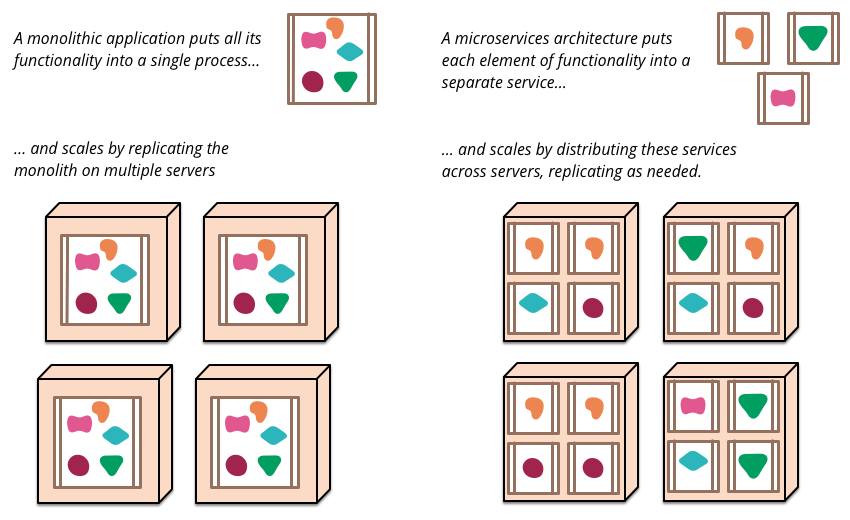
\includegraphics[width=0.8\textwidth]{estruturaMicrosservicos}
\label{fig:estruturaMicrosservicos}
\end{figure}

É difícil delimitar uma definição formal para arquitetura de microsserviços, pois não existe consenso a respeito de sua definição formal. Contudo, existe uma série de características que projetos usando essa arquitetura compartilham. Detalhamos a seguir alguns atributos e aspectos dos microsserviços. Nem todos os projetos possuem rigorosamente todas as características, mas a maioria deles possui um perfil similar ao descrito aqui.

\begin{itemize}
\item \textbf{Serviços são processos. }Pode-se fazer um mapeamento de um processo para um serviço, porém isso é apenas uma aproximação, podendo um serviço ser constituído por uma aplicação de múltiplos processos.
\item \textbf{Serviços comunicam-se por protocolos leves. }Geralmente, são usados protocolos como o HTTP.
\item \textbf{Serviços implementam capabilidades do negócio. }Isto é, a divisão de serviços é baseada nas regras de negócio e nas funcionalidades que o produto deverá suprir.
\item \textbf{Serviços são facilmente substituíveis.}
\item \textbf{Cada serviço tem um ciclo de vida independente. }Isso inclui o desenvolvimento e os processos de deploy. Um microsserviço pode ser implementado e atualizado independentemente dos outros.
\end{itemize}

As vantagens da arquitetura de microsserviços giram em torno da modularidade e autonomia dos serviços que é natural à sua estrutura. Com isso, pode-se ter uma heterogeneidade de tecnologias, isto é, cada serviço pode ser desenvolvido usando diferentes linguagens, frameworks e ferramentas de acordo com seus requisitos. A independência entre serviços também possibilita o deploy automatizado e o uso de práticas de integração contínua. Também há benefícios de aspecto gerencial: como cada serviço tem como escopo uma capabilidade do negócio que envolve interfaces de interação com usuário, código em várias camadas que implementa as funcionalidades necessárias e persistência em bancos de dados, é possível criar pequenas equipes multidisciplinares para cada microsserviço.

Building for failure % TODO

Existem trade-offs que devem ser considerados ao decidir pela arquitetura de microsserviços. A comunicação entre serviços por meio de uma rede possui maior latência e exige maior processamento do que mensagens trocadas a nível de processos. Por isso, é muito importante analisar as fronteiras dos serviços e a alocação de responsabilidades durante do projeto. A descentralização de dados entre microsserviços traz também a necessidade de métodos para manter a consistência das informações. Outro ponto crítico são sistemas com alta granularidade de microsserviços, causando overhead tanto de comunicação como de código além de uma fragmentação lógica que causa mais impactos negativos na complexidade e performance do que benefícios - tal caso de antipadrão foi chamado de nanosserviço \cite{rotem}.

% TODO melhorar paragrafo abaixo
Os microsserviços podem ser vistos como um estilo específico de arquitetura orientada a serviços (Service-oriented architecture - SOA), visto que existem várias características compartilhadas entre os dois. Contudo, o termo arquitetura orientada a serviços é muito amplo, e muitas de suas implementações podem não seguir certos pontos apresentados como aspectos dos microsserviços, como por exemplo, o uso de grande inteligência no mecanismo de comunicação de dados ao invés de delegar tal complexidade aos endpoints do serviço \cite{james}. Esse e outros problemas conhecidos das experiências passadas de sistemas estruturados em SOA fazem com que muitos encarem os microsserviços como uma modernização da arquitetura orientada a serviços.

Apesar do termo microsserviço ter surgido por volta de 2011 \cite{james}, as ideias por trás desse estilo arquitetural não são recentes. O aumento da discussão em torno dos microsserviços nos últimos anos pode ser creditada a avanços tecnológicos tais como a disseminação dos serviços de nuvem, o crescimento de ferramentas de automatização de deployment, a consolidação dos conceitos de DevOps, entre outros.

\subsubsection{Casos de uso} % TODO

\subsubsection{Microsserviços e Internet das Coisas} % TODO

\section{Cliente Web}
Para criar aplicações web que demonstrem as funcionalidades dos módulos de automação da casa, foi escolhida a biblioteca de JavaScript React, que permite o fácil desenvolvimento de aplicações single-page, renderizadas do lado do cliente, e que permitem a atualização dinâmica da página, de forma fluida, rápida, o que acaba enriquecendo a experiência do usuário na aplicação (UI e UX). Esse cliente irá se comunicar com a API, por meio do protocolo HTTP, e utilizando autenticação de usuário por meio  de tokens do tipo JSON Web Token. JSON Web Tokens são tokens gerados no cadastro ou login do usuário, e são enviados ao browser, onde são armazenados na Localstorage do mesmo.

A partir desse momento, todas as requisições ao back end conterão tal token no campo de Authentication do cabeçalho dos métodos HTTP (GET, PUT, POST, DELETE). Somente requisições contendo tal token, e cujo token seja válido, são aceitas.

Outro ponto interessante para a utilização da biblioteca React é que, com a biblioteca React Native - uma extensão da biblioteca React - é possível a geração de aplicativos nativos para iOS e Android, que podem vir a ser desenvolvidos no desenrolar do projeto. Isso diminui a necessidade de retrabalho e dispensa a necessidade de estudo aprofundado das linguagens e ambientes de desenvolvimento tradicionais de projeto de aplicativos nativos.

\section{App Backup}
\subsection{Interface}
\subsection{Setup}
\subsection{Abertura de porta do roteador}
\subsection{Configurações}
\subsection{Serviços essenciais}

\section{Comunicação}
Conforme explicado anteriormente, neste projeto utilizamos tanto protocolos de comunicação próprios quanto os elaborados comercialmente. A arquitetura desenvolvida aqui busca viabilizar a robustez do sistema, trabalhando em um nível local e outro nível remoto, onde o usuário terá o controle de sua casa por meio do Smartphone ou computador pessoal.

Teremos um serviço de nuvem (que será descrito na seção de software) que receberá as requisições do usuário, por meio de um cliente web ou nativo. Esse servidor processará as requisições, aplicando os filtros de segurança necessário, de modo a consultar a autenticidade do pedido, e se aquele usuário possui as permissões necessárias para o serviço que deseja operar. Os serviços da nuvem se comunicarão com o servidor local, da casa requisitada, o qual também aplicará os filtros de segurança necessários, e realizará a comunicação com os atuadores.

A infraestrutura de comunicação entre a nuvem e o servidor local, e o servidor local e os sensores e atuadores utilizará o protocolo de aplicação MQTT, referência em aplicações IoT no mundo. O protocolo MQTT é estabelecido em cima dos protocolos TCP/IP (nas camadas inferiores) e é orientado é orientado à sessão, diferentemente do protocolo HTTP, de mesma camada.

O protocolo MQTT é do tipo Pub/Sub (de publisher/subscriber) e é estritamente orientado à tópicos. Assim, um subscriber deve se inscrever a um tópico de seu interesse, e receberá todas as publicações que um publisher realizar. Os tópicos são organizados com estrutura semelhante a de um sistema de arquivos Unix, com níveis hierárquicos, separados por barras, de modo que o subscriber pode se inscrever para tópicos utilizando wildcards (* e +, os quais são válidos para mais de um nível e um único nível, respectivamente).

Para interconectar os tópicos, com publishers e subscribers, é necessário um agente que realiza a transmissão das mensagens, e que garante a segurança e confiabilidade. Esse agente é conhecido como Broker (em versões anteriores) ou Server (na versão atual, V3.1.1). O broker irá permitir ou negar a subscrição a determinado tópico, ou a publicação.

A segurança da troca de mensagens é realizada por meio do protocolo TLS (Transport Layer Security) que encripta os segmentos na camada de transporte. Toda a parte de segurança e criptografia será detalhada no momento oportuno, bem como a organização dos tópicos implementados.

Além disso, o protocolo MQTT oferece três tipos de QoS (Quality of Service), possibilitando: diminuir o overhead ao máximo, enviando a mensagem uma única vez, na configuração mais simples; garantir que a mensagem seja entregue no mínimo uma vez, na configuração de segundo nível; garantir que a mensagem seja entregue exatamente uma vez, no terceiro nível, o que aumenta o overhead, consequentemente.

As mensagens são transmitidas em texto puro, e é necessário estabelecer um protocolo para a sua utilização. Utilizaremos aqui o protocolo que define a configurações das mensagens, desenvolvido no projeto HomeSky.

O broker Mosquitto será utilizado, e foi escolhido por ser amplamente adotado em projetos de IoT, além de ser open source e com licença abrangente (MIT). Entretanto, há diversas possibilidades, como o HiveMQ, adotado no projeto HomeSky, e com grande uso em aplicações enterprise.

A arquitetura de comunicação é representada pelo diagrama abaixo, com um alto nível de abstração, cujos detalhes serão vistos no momento oportuno, com granularidade menor.

% TODO o diagrama ta diferente no arquivo da quarta entrega
\begin{figure}[H]
	\centering
	\caption{}
  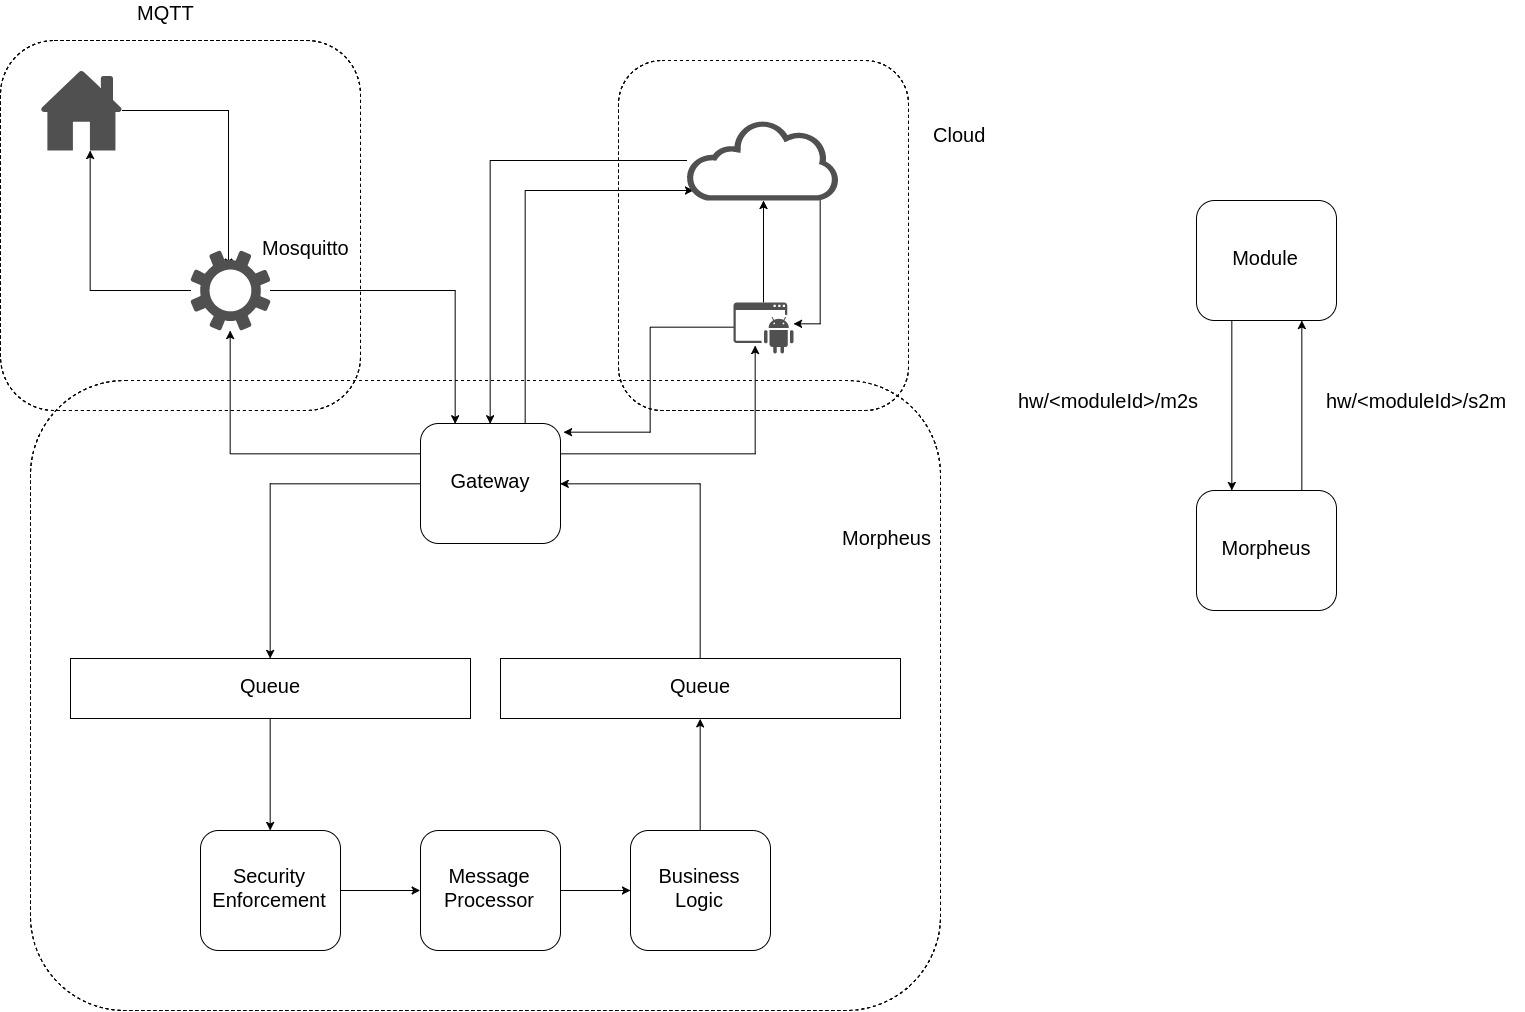
\includegraphics[width=0.8\textwidth]{diagramaComunicacao}
\label{fig:diagramaComunicacao}
\end{figure}

\subsection{Entre módulos e controlador local}
\subsection{Entre controlador local e nuvem}
\subsection{Entre cliente web e nuvem}
\subsection{Entre app backup e módulos}

\chapter{Metodologia}

\section{Gerência do Projeto}

Para realizar a gerência do projeto Hedwig, foram usadas certas diretrizes do PMBOK \cite{pmi} e da norma ISO/IEC 12207 \cite{iso12207} como referência para coordenar os processos.

\subsection{Gerência de Escopo}

Segue a EAP (Estrutura Analítica do Projeto), que orientou as entregas realizadas e escopo do projeto.

\begin{figure}[H]
	\centering
	\caption{EAP do Hedwig}
	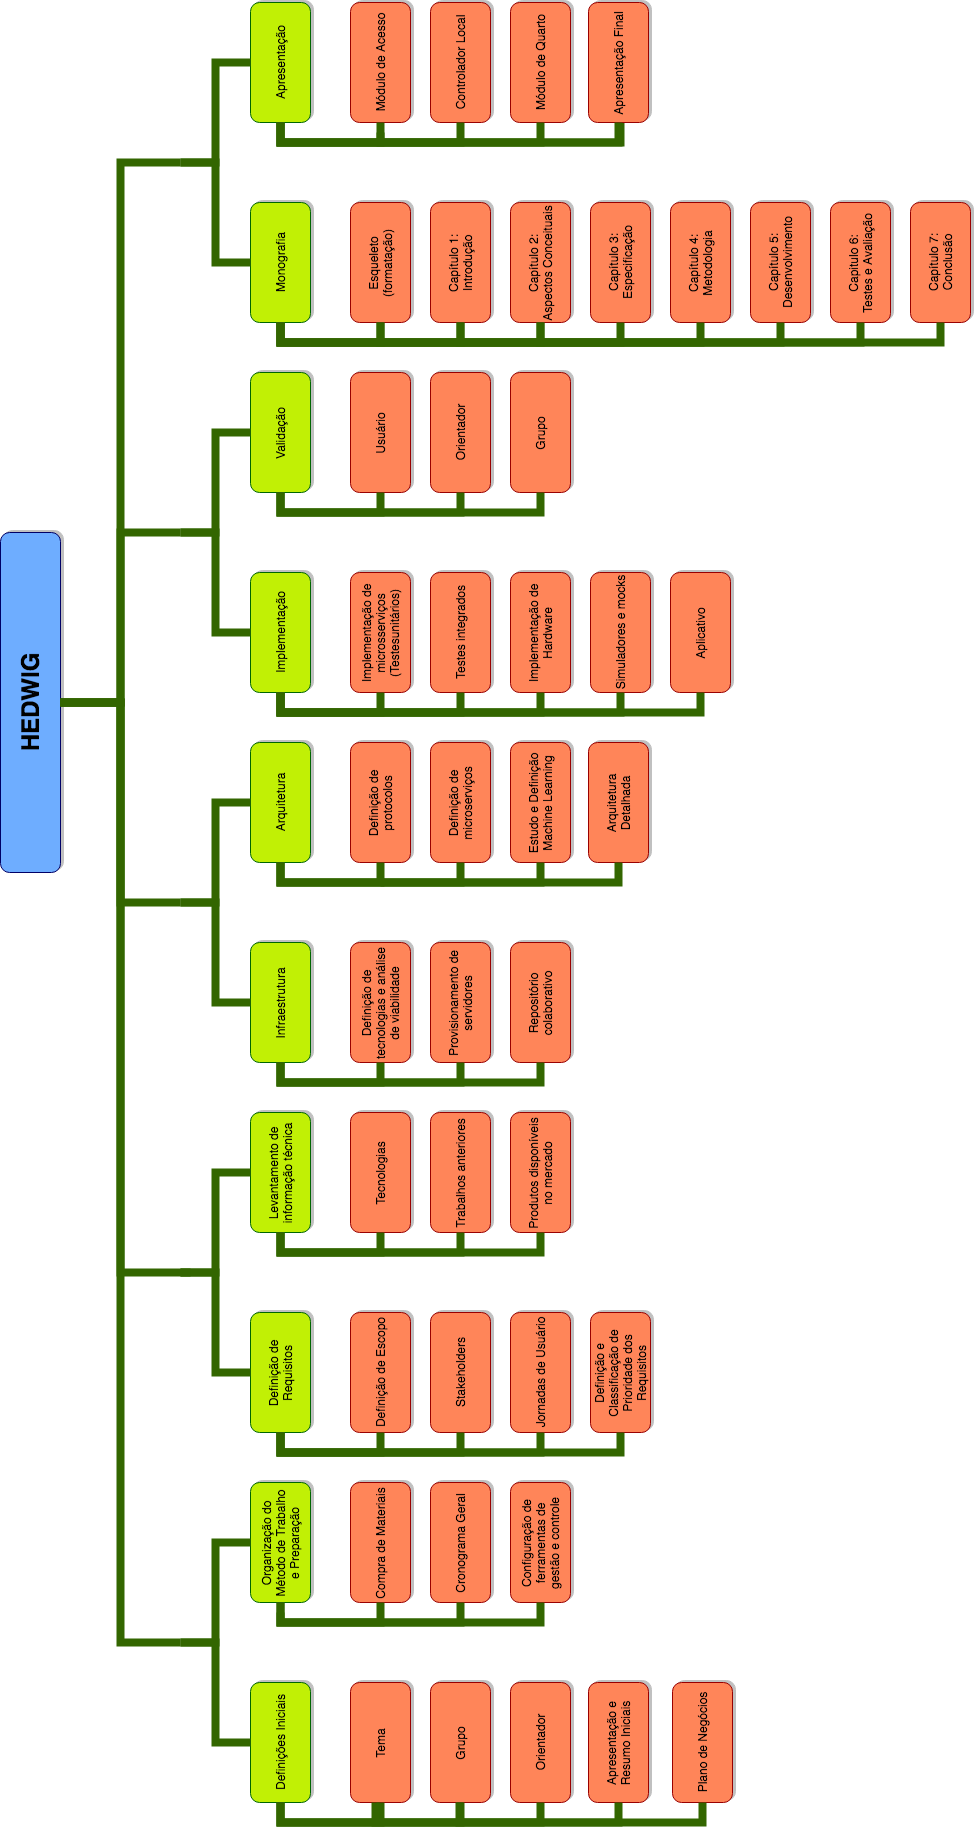
\includegraphics[width=0.8\textwidth]{Hedwig_EAP}
	\label{fig:Hedwig_EAP}
\end{figure}

\subsection{Gerência de Aquisição}

O gerenciamento de aquisições envolve primariamente a compra dos materiais necessários para implementação dos módulos físicos. Foi necessário analisar o que adquirir e como fazê-lo, levando em consideração as limitações de tempo do projeto --- a demora ou atraso na entrega dos componentes eletrônicos causaria um atraso no cronograma. A escolha dos fornecedores priorizou, então, o custo e o prazo de entrega.

A relação de materiais necessários para a confecção de um módulo básico encontra-se no Apêndice \ref{listamateriais}.

\subsection{Gerência de Processos de Software}

Para gerenciar o código-fonte e permitir o trabalho da equipe em múltiplas partes do projeto ao mesmo tempo, foi utilizado o Git, um sistema de controle de versão distribuído. Para publicação do código, foi escolhido o GitHub, onde criou-se a organização Hedwig\footnote{https://github.com/hedwig-project} e os repositórios que contém o código das diversas partes do sistema. A preferência pelo GitHub se deu pelas suas funcionalidades de gerenciamento e colaboração, como a notificação de \emph{bugs}, acompanhamento do progresso de tarefas e criação de \textit{wikis}, além de ser uma plataforma conhecida por abrigar grandes projetos \emph{open-source} que chegam a ter centenas ou milhares de contribuidores \cite{github}. O GitHub disponibiliza também uma ferramenta para armazenamento de \emph{Issues} --- atividades que necessitam ser observadas ou desenvolvidas em um projeto. Esse recurso foi essencial na organização de tarefas e rastreamento de mudanças em curso.

Para a coordenação de trabalho nesses repositórios, foi utilizado o fluxo conhecido como \textit{Feature Branch Workflow} \cite{atlassian}, caracterizado pela criação de \textit{branches} (ramificações) para o desenvolvimento de cada nova funcionalidade. Ao final do desenvolvimento de cada funcionalidade, é feito um pedido para mesclar à \textit{master branch}, ramificação principal, o código desenvolvido na ramificação atual --- conhecido como \emph{Pull Request}. A utilização de \emph{Pull Requests} promove maior controle sobre a atualização do código mantido, e também promove a revisão do código pelos aprovadores. 

Já outros tipos de documentação formal do sistema, como textos e planilhas, foram editados e armazenados no Google Drive\footnote{https://www.google.com/drive/}, ferramenta de armazenamento e backup da Google que também permite colaboração, compartilhamento e controle de versão.

\subsection{Gerência de Comunicação}

Para comunicar as tarefas, estudos e pesquisas sendo realizadas durante o projeto, foi utilizado o Trello\footnote{https://trello.com/}, um sistema online para organização de ideias e projetos, que permite listagem e acompanhamento das atividades a serem realizadas, permitindo a adição de prazos, delegação de responsáveis e categorização das tarefas.

Foram realizadas diversas reuniões online usando ferramentas de videoconferência, como o Google Hangouts\footnote{https://hangouts.google.com} e o Skype\footnote{https://www.skype.com}, que, além do \emph{streaming} de vídeo com áudio, possuem funcionalidades como mensagens de texto, envio de arquivo e compartilhamento de tela, facilitando demonstrações e testes integrados.

\subsection{Gerência de Riscos}

Para gerenciar os riscos do projeto, foram realizadas reuniões periódicas com participação das partes interessadas --- grupo e orientadores --- nas quais discutiam-se táticas de análise, planejamento e monitoramento. Nessas sessões, foi possível identificar riscos por meio da revisão da documentação e de técnicas de \emph{brainstorming} e definir estratégias de abordagem de riscos.

\section{Pesquisa Bibliográfica}

O estudo dos tópicos relacionados a aprendizagem de máquina foi realizado com auxílio do curso \emph{Aprendizagem Automática}, do Professor Andrew Ng\footnote{ https://www.coursera.org/learn/machine-learning}, oferecido pela Universidade de Stanford e disponibilizado no Coursera, uma plataforma de MOOCs (\textit{Massive Open Online Courses}) que oferece cursos abertos e especializações. O livro ``Introduction to Statistical Learning in R'' \cite{islr} também foi amnplamente utilizado para aprendizado nessa área.

Os cursos da especialização em \textit{Data Science} da Universidade Johns Hopkins\footnote{ https://www.coursera.org/specializations/jhu-data-science}, também disponíveis no Coursera, foram usados como referência e treinamento para realizar a coleta de dados de maneira metódica. Por esse motivo, foi dada maior atenção ao curso \textit{Getting and Cleaning Data}. Contudo, também foi aproveitado conteúdo do curso \textit{Practical Machine Learning}.

\section{Ferramentas e Tecnologias}

Para a aprendizagem da biblioteca React, para o desenvolvimento do \emph{front-end}, foi usada como referência a documentação oficial\footnote{https://facebook.github.io/react/docs/hello-world.html} oferecida pelo Facebook e o curso \textit{React for Beginners} de Wes Bos\footnote{ https://reactforbeginners.com/}. O aprendizado de Redux foi auxiliado pelo curso \textit{Learn Redux}\footnote{https://learnredux.com}, do mesmo autor. O conhecimento necessário à utilizaçãodo Spring Boot foi obtido com base no guia de referência oficial\footnote{https://docs.spring.io/spring-boot/docs/current/reference/htmlsingle/}.

O aprendizado para uso de outros \emph{frameworks}, ferramentas e tecnologias citadas ao longo deste documento foi altamente baseado em documentações oficiais dos mesmos disponibilizados gratuitamente em páginas na Internet, além de diversos tutoriais disponibilizados pela comunidade que utiliza tais ferramentas e tecnologias.

\section{Método de Testes}

A estratégia de testes utilizada está fortemente relacionada com a estratégia de desenvolvimento. A implementação do projeto foi realizada em partes, segregadas de acordo a área de aplicação. Assim, as diversas frentes puderam ser desenvolvidas em paralelo, como os módulos, servidor local, aplicativo cliente, etc. juntamente com os seus respectivos testes.

Para cada tarefa específica foram efetuados testes unitários, de pequeno alcance, para validar a funcionalidade ou alteração. O desenvolvimento do servidor local contou também com testes unitários automatizados, entretanto sem cobertura do sistema inteiro. Para testes específicos dos \emph{endpoints} do servidor na nuvem foi utilizada a ferramenta Postman\footnote{https://www.getpostman.com/}, que permite simular requisições a tais \emph{endpoints}, configurando todos os parâmetros necessários e informações de cabeçalho HTTP, e apresenta ao usuário a resposta recebida.

Durante a integração das partes, houveram diversos testes ponto-a-ponto, para verificação do funcionamento completo do sistema. Utilizou-se para isso o Software MQTT Fx\footnote{http://mqttfx.jensd.de/}, onde é possível obter as mensagens encaminhadas pelo sistema de mensageria, e compará-las com os resultados esperados. Na Subseção \ref{testesTopicos} são mostrados alguns casos de testes utilizados durante a configuração do Broker Mosquitto, enquanto a seção \ref{atttestefimafim} contém um exemplo de teste fim a fim realizado com aplicativo, servidor local, nuvem e módulo.

Com a instalação do sistema em duas residências distintas, houve uma validação contínua de premissas e levantamento de requisitos, principalmente aqueles relacionados à usabilidade. Foram realizados diversos testes de conceito em campo, de forma que muitas soluções, embora fizessem sentido experimentalmente em implementações isoladas, não eram adequadas para módulos instalados em uma residência real. Ainda, atualizações e melhorias foram entregues frequentemente, contribuindo para o crescimento iterativo do projeto (destacam-se a aplicação dos princípios 2 e 4 do Agile Manifesto\footnote{http://agilemanifesto.org/iso/ptbr/manifesto.html}, que dissertam sobre mudanças frequentes de requisitos e entregas frequentes de software).

Em especial, o contato do desenvolvedor dos módulos com todos os problemas e desafios encontrados com o uso do sistema em sua residência facilitou sua proximidade com um dos stakeholders principais, possibilitando um \textit{feedback} rápido, reduzindo o ciclo de desenvolvimento consideravelmente.

\chapter{Implementação}

\section{Morpheus}

\subsection{Descrição}
%TODO add source below
Morpheus é o servidor local responsável pela interconexão da casa inteligente com os serviços de nuvem. O nome tem sua origem na mitologia grega, onde o Deus dos sonhos, Morpheus, era responsável pelo envio de mensagens entre dois mundos diferentes, o dos deuses e o dos mortais [TODO add source]. Sua principal atribuição é garantir que a troca de mensagem entre os módulos e a nuvem seja realizada com segurança e confiabilidade, munindo-se de soluções robustas para desempenhar o seu papel.

\subsection{Plataforma}
O Morpheus tem seu desenvolvimento realizado em Java. Conforme será detalhado em seguida, tal escolha foi realizada com base na portabilidade que a máquina virtual Java (JVM) oferece, bem como na disponibilidade de bibliotecas e serviços largamente utilizados em aplicações comerciais. O servidor foi construído utilizando-se o Spring Boot Framework, com a utilização de seu container de Inversão de Controle (\textit{IoC - Inversion of Control}), para injeção de dependências. Essa técnica diminui o acoplamento entre classes, e permite a evolução e implementação de novas funcionalidades de maneira mais facilitada.

Para se comunicar com os módulos, o Morpheus utiliza-se da conexão com um \textit{broker} \wmqtt{}. O \textit{broker} que utilizamos é o Mosquitto, por ser uma solução Open Source largamente utilizada em projetos de Internet das Coisas. Conforme detalhado a frente, configurações de segurança específicas para nosso projeto foram registradas no \textit{broker}. Para a conexão com os serviços na nuvem, é utilizado um canal WebSocket, aberto pelo Morpheus (cliente) e aceito pela nuvem (servidor). Esta solução veio a partir de uma discussão em relação à segurança, a qual está documentada aqui. Na figura a seguir, é possível verificar a arquitetura desenvolvida.

% TODO cade a figura que foi citada na linha acima?

\subsection{Tecnologias utilizadas}
Toda a implementação do Morpheus foi realizada na linguagem Java. Desde o começo do projeto, decidiu-se que a escolha de tecnologias para implementação das diversas camadas deveria ter por base os seus benefícios, e não necessitaria ser rígida ou uniforme. Assim, o principal esforço foi sempre no planejamento das interfaces de comunicação entre as partes, que poderiam ser desenvolvidas em linguagens complementamente diferentes. Os sistemas de nuvem, por exemplo, foram implementados em Node.js. O aplicativo web, também em JavaScript, com utilização da biblioteca React. Os módulos de hardware foram programados em C e, como comentado acima, o controlador local em Java.
Essa flexibilidade permitiu que fossem utilizados os recursos e tecnologias que fossem melhores integrados com os requisitos propostos.

Um requisito essencial para o controlador local é a sua robustez. Em um cenário em que este controlador não esteja disponível, a casa passa a funcionar em estado de emergência, onde os comandos são reduzidos, e não permitem acesso remoto. Entretanto, há inúmeras possibilidades e eventos que poderiam causar a queda deste controlador, muitas das quais referem-se a situações fora de nosso alcance. A falta de energia na residência, ou de Internet, interrompe o seu funcionamento, e não é possível ter controle sobre tal situação. O mesmo ocorre no evento de problemas de hardware, na plataforma que o sistema estiver rodando. Além do fato de que tais situações estão fora de nosso controle, os planos para contenção dos seus efeitos são complexos, custosos e fogem do escopo deste projeto, como seria o caso de se implementar duplicações, banco de baterias e tecnologia celular para comunicação secundária.

Há, entretanto, problemas no software que poderiam afetar o funcionamento do controlador. Por meio de testes, muitos desses problemas podem ser evitados, ainda em tempo de desenvolvimento. A utilização de tecnologias que facilitam o desenvolvimento seguro da aplicação é uma vantagem para este caso, já que ferramentas estão disponíveis para que haja maior controle sobre o código desenvolvido, e pode-se detectar erros mais facilmente, ainda em tempo de compilação, por exemplo.

O controlador local também precisa lidar com as requisições assíncronamente. Parte desta tarefa é facilitada com a utilização do sistema de mensageria \wmqtt{}, operado pelo \textit{broker} Mosquitto. Com sua utilização, mensagens podem ser enviadas, e mesmo que o controlador não consiga recebê-las, elas não serão perdidas. Entretanto, devido às características do sistema proposto, as mensagens precisam ser operadas sem maiores demoras. O controlador deve receber e processar as mensagens paralelamente, e não esperar o processamento de uma mensagem inteira, para assim processar a próxima, de modo que paralelismo deve ser parte essencial da arquitetura.

Ainda, para a integração com os serviços da nuvem, é necessário a utilização de JSON, para a serialização das mensagens, em um formato que pode ser desserializado posteriormente, independentemente da plataforma. Para a utilização de WebSockets, é necessário o uso de bibliotecas disponíveis, de modo que o desenvolvimento seja facilitado. Por último, é necessário gerenciar eficientemente todas essas dependências. Atualizá-las quando necessário, ou substituí-las, se desejado, deve ser uma tarefa simples.

A arquitetura oferecida pelo Java mostra ser efetiva para as necessidades levantadas acima. Com a utilização de uma IDE avançada, inúmeros recursos estão disponíveis para limpeza, refatoração, organização do código, etc. O \textit{framework} Spring Boot\footnote{https://projects.spring.io/spring-boot/} foi utilizado para o desenvolvimento, por oferecer diversos recursos que facilitam o desenvolvimento, com configurações de ambiente e o oferecimento de um \textit{container} para inversão de controle e injeção de dependência\footnote{https://martinfowler.com/articles/injection.html}. Além disso, o gerenciador de dependências Gradle\footnote{https://gradle.org/} foi também utilizado, por oferecer um poderoso ambiente para configurar, construir e distribuir aplicações. Gradle faz uso de Groovy\footnote{http://groovy-lang.org/}, tecnologia que também roda na \textit{Java Virtual Machine} (JVM). Por outro lado, o uso de tais ferramentas e plataformas necessita de hardware mais robusto, para que funcione, sendo uma desvantagem. Entretanto, frente aos benefícios, ainda é vantajoso a utilização de Java, neste caso.

Java é utilizado em vasta gama de aplicações, deste complexos softwares comerciais como a IDE Eclipse, até software embutidos, como controladores de BlueRay\footnote{http://www.oracle.com/technetwork/articles/javame/bluray-142687.html}.
O padrão de inversão de controle, com injeção de dependências, foi utilizado para o desenvolvimento, de modo a diminuir o acoplamento entre as partes, e facilitar futuras modificações. Assim, cada módulo recebe, em seu construtor, todas as dependências que serão utilizadas. A responsabilidade da construção de tais dependências passa, então, a ser responsabilidade do gerenciador de contexto, e não mais do módulo. A escolha do Java 8 foi decidida para que o desenvolvimento possa utilizar certos recursos de paradigmas funcionais, como o conceito de Streams de dados e Funções Lambdas.

Internamente, o Morpheus é dividido em pacotes, que são responsáveis pela modelagem do problema. Há classes que modelam o domínio, que executam as regras de negócio, que fazem a interface entre outros sistemas (\wmqtt{} Mosquitto Broker e nuvem), e que fazem a execução de tarefas como backup de mensagens, e serviços de conversão.
Assim que uma mensagem chega ao Morpheus, ela é reconhecida e é realizado o seu parsing, para as estruturas de domínio internas. Caso haja algum erro, para mensagens vindas da nuvem, há o envio de relatório com os problemas encontrados. A partir daí, a mensagem é colocada em uma fila interna, onde outro módulo será responsável por capturá-la e realizar o processamento necessário.

\begin{figure}
	\centering
	\caption{Arquitetura do servidor local}
  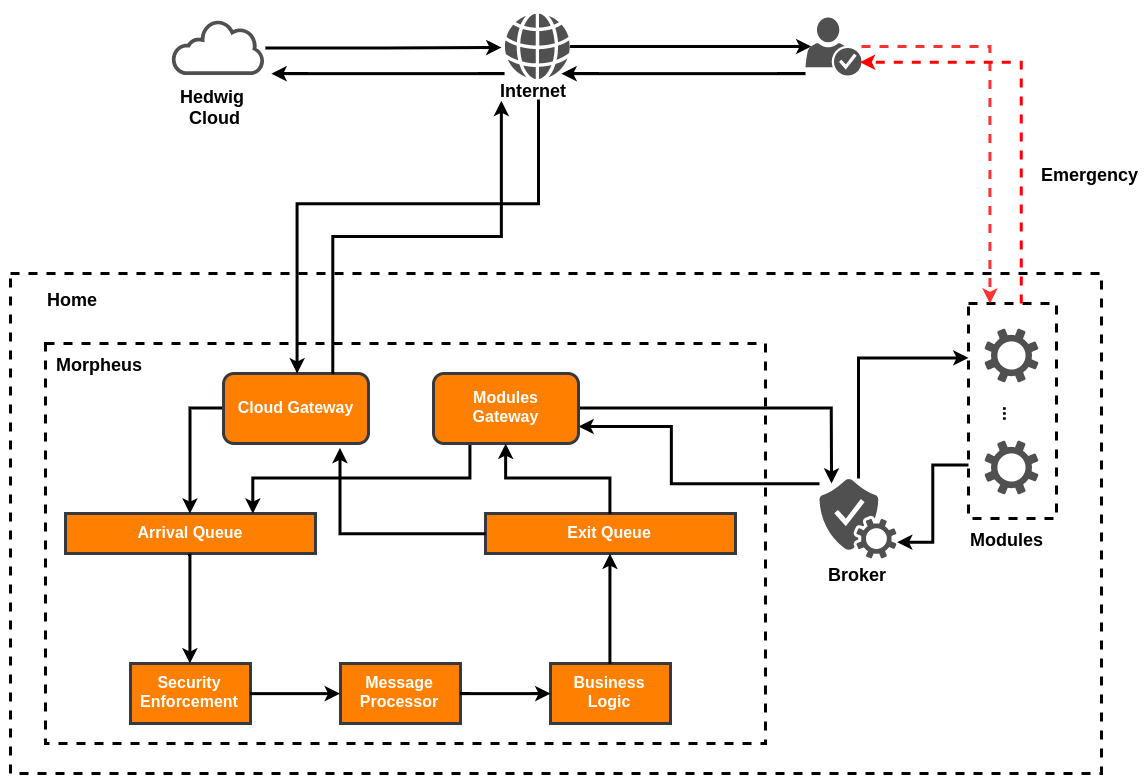
\includegraphics[width=\textwidth]{diagramaDeComunicacao}
\label{fig:diagramaDeComunicacao}
\end{figure}

\subsection{Requisitos}
Para a concepção do servidor local, foram discutidos os seus requisitos funcionais e não funcionais, bem com suas prioridades na implementação.

\subsubsection{Requisitos Funcionais}
\begin{description}

\item \textbf{Configuração dos módulos físicos}

De acordo com as regras e interfaces estabelecidas, documentadas aqui, os módulos podem ser configurados por meio de mensagens. Os serviços da nuvem enviarão os parâmetros de configuração de cada módulo ao Morpheus, que os transmitirá ao módulo.

\item \textbf{Conexão de emergência}
% TODO (gabi falando) não sei se esse é um requisito do Morpheus, isso pra mim tem a ver com a arquitetura geral do sistema. Pro Morpheus deveria não importar se os módulos podem ser controlados de outra forma ou não

Quando não há conexão da casa com a nuvem, deverá haver um canal para comunicação local entre o aplicativo e alguns dos módulos, com funcionalidades limitadas, apenas para serviços essenciais.

\item \textbf{Envio de dados para a nuvem}

Dados provenientes de sensores são enviados para a nuvem, para que sejam tratados de acordo com as regras de Business Intelligence, e utilizados em algoritmos de Machine Learning.

\item \textbf{Persistência de dados}

Quando não houver conexão, o servidor deverá armazenar os dados localmente e, quando solicitado, enviá-los à nuvem.

\item \textbf{Tentativas de reenvio}

Quando uma mensagem não é enviada com sucesso à nuvem, o Morpheus deverá tentar novamente, por um número configurável de vezes, em um
curto espaço de tempo. Isso ocorre pois se determinada mensagem não pode ser enviada em uma janela temporal, ela perde o seu sentido, bem como por questões de segurança.

\item \textbf{Envio de e-mail}

Se o Morpheus estiver desconectado da nuvem por um período, configurável, deverá avisar o usuário, por meio de uma mensagem de e-mail.

\item \textbf{Verificação do time-stamp}

Quando uma nova mensagem chegar, seu timestamp deverá ser verificado, e a mensagem tomará curso somente se não for obsoleta.

\item \textbf{Tomadas de ação}

Quando o usuário requisitar uma tomada de ação, esta deverá ser enviada por meio de uma mensagem ao Morpheus, o qual a transmitirá ao módulo.

\item \textbf{Configuração em arquivo}

As configurações básicas do Morpheus devem ser registradas em um arquivo YAML, que será lido durante a inicialização.

\item \textbf{Listeners para diferentes tipos de mensagens}

Deverão haver \textit{listeners} para todos os tipos de mensagens, definidos aqui, que serão recebidos da nuvem e dos módulos.

\end{description}

\subsubsection{Requisitos Não Funcionais}
\begin{description}
\item \textbf{Processamento concorrente}

Toda a infraestrutura do Morpheus deverá permitir o processamento de mensagens de maneira concorrente. Não deve ser permitido esperar o processamento completo de uma mensagem para que outra comece a ser processada.

\item \textbf{Utilização de criptografia na troca de mensagens com a nuvem}

Os dados que trafegam entre a nuvem e o servidor local não devem ser codificados em texto puro. Devem estar protegidos contra \textit{sniffers}.

\item \textbf{Conversão de mensagens}

As mensagens enviadas à nuvem devem estar em formato JSON, e não no protocolo definido aqui, que refere-se apenas à troca de mensagens entre os módulos e o Morpheus.

\item \textbf{Serialização das configurações}

O servidor deverá serializar e persistir as configurações relativas aos módulos que foram configurados, e carregá-las em sua inicialização.

\item \textbf{Destruição de pools de threads}

Ao ser desligado, todos os \textit{pools} de \textit{threads} criados devem ser destruídos.

\end{description}

\subsection{Especificações}

\subsubsection{Tópicos}
Todos os tópicos devem seguir o formato especificado abaixo. Com essa formatação, é possível garantir que:

\begin{enumerate}
\item Somente o Morpheus conseguirá publicar em qualquer tópico, ou ser um \textit{subscriber} de qualquer tópico.
\item Cada módulo somente consiga publicar no tópico determinado para ele, que será garantido com as credenciais (usuário e senha) fornecidos pelo tópico.
\item Caso um módulo malicioso seja implantado, com o roubo das credenciais de um módulo legítimo, o impacto será unicamente concentrado naquele tópico, não atingindo outros módulos.
\end{enumerate}

Temos as seguintes regras:

\textbf{hw/\textless ID do módulo\textgreater /s2m} (Server to Module - o módulo deve ser \textit{subscriber} desse tópico. O servidor deve ser \textit{publisher} desse tópico).

\textbf{hw/\textless ID do módulo\textgreater /m2s} (Module to Server - o servidor deve ser \textit{subscriber} desse tópico. O módulo deve ser \textit{publisher} desse tópico).

\subsubsection{Regras de negócio}
O servidor foi desenvolvido com base nas regras de negócio seguintes.
\begin{enumerate}
\item Após a compra de cada módulo, o usuário deverá registrar online a aquisição. O servidor da nuvem enviará para o servidor local, da casa, a requisição para configurar o módulo.
\item Cada módulo enviará mensagens para o servidor local com o seus dados, por meio do \wmqtt{}.
\item Para a troca de senha do \wwifi, o usuário cadastra no site a nova senha. O servidor na nuvem faz a requisição para o servidor local, o qual enviará um arquivo de configuração com a nova senha para cada um dos módulos registrados. Após a configuração de todos os módulos, o servidor local envia resposta de sucesso para a nuvem, a qual indica ao usuário que a troca de senha já pode ser feita com sucesso.
\item Todo módulo sai de fábrica configurado com o tópico que deve se inscrever e publicar, com base no seu ID, o qual será o seu usuário, e também haverá a senha para se autenticar junto ao \textit{broker} \wmqtt{}.
\end{enumerate}

\subsubsection{Definição de interfaces}
\begin{itemize}
\item Há três tipos de mensagens que vão do Morpheus para os módulos:
  \begin{itemize}
  \item Configuração (configuration)
  \item Requisição de Ação (action\_request)
  \item Requisição de dados (data\_transmission)
  \end{itemize}
\item Há três tipos de mensagens que chegam dos módulos:
  \begin{itemize}
  \item Confirmação (confirmation)
  \item Envio de Dados (data\_transmission)
  \item Data Request (data\_request)
  \end{itemize}
\end{itemize}

\subsubsection{Definição das mensagens}
\paragraph{Configuração (configuration)}
\begin{itemize}
\item Sentido: Morpheus para módulo
\item Uso: Envio de parâmetros para configuração dos módulos.
\end{itemize}

\textbf{Configuração de hora:}
\begin{lstlisting}
#configuration
$ts: <timestamp>
$ty: time_config
@
updated_ntp: <segundos desde 0h de 1 de Janeiro de 1970, 64 bits>
@
\end{lstlisting}

\textbf{Configuração de nome:}
\begin{lstlisting}
#configuration
$ts: <timestamp>
$ty:name_config
@
new_name: <nome>
new_rele1name: <nome | "">
new_rele2name: <nome | "">
@
\end{lstlisting}

\textbf{Configuração de comunicação:}
\begin{lstlisting}
#configuration
$ts: <timestamp>
$ty: comunication_config
@
new_ssid: <novo_SSID>
new_password: <nova_senha>
ip_local: <novo_IP_local>
ap_mod: <"sempre ativo" | "automatico">
ap_name: <nome_AP_acesso_direto>
ap_password: <senha_AP_acesso_direto>
@
\end{lstlisting}

\textbf{Configuração de RF:}
\begin{lstlisting}
#configuration
$ts: <timestamp>
$ty: rf_config
@
*
<nome_do_[sensor | controle | funcao]>: "store" | "clear" | "keep"
*
@
\end{lstlisting}

\textbf{Configuração de display:}
\begin{lstlisting}
#configuration
$ts: <timestamp>
$ty: display_config
@
displaytype: <1 | 2 | 3>
backlight: <0 | 1>
@
\end{lstlisting}

\paragraph{Requisição de ação (action\_request)}
\begin{itemize}
\item Sentido: Servidor para módulo
\item Uso: Quando um usuário faz a requisição de uma ação por meio do aplicativo. Por exemplo, quando deseja-se acender uma luz, o aplicativo envia uma requisição para o servidor local, o qual enviará uma mensagem de action\_request para o módulo correspondente.
\end{itemize}

\textbf{Requisição de acionamento:}
\begin{lstlisting}
#action_request
$ts: <timestamp>
$ty: rele1_action
@
rele1: <0 | 1>
@
\end{lstlisting}

\begin{lstlisting}
#action_request
$ts: <timestamp>
$ty: rele2_action
@
rele2: <0 | 1>
@
\end{lstlisting}

\textbf{Requisição de SW Restart:}
\begin{lstlisting}
#action_request
$ts: <timestamp>
$ty: sw_reset
@
swreset: <0 | 1>
@
\end{lstlisting}

\textbf{Requisição de Teste de Auto Reset:}
\begin{lstlisting}
#action request
$ts: <timestamp>
$ty: autoreset_test
@
autoreset: <0 | 1>
@
\end{lstlisting}

\textbf{Confirmação (confirmation)}
\begin{itemize}
\item Sentido: Do módulo para o servidor
\item Uso: Confirmação de uma configuração, patch ou requisição de ação, vindas do servidor.
\end{itemize}

\textbf{Confirmação de hora}
\begin{lstlisting}
#confirmation
$ts: <timestamp>
$ty: time_confirm
@
ntp: <segundos desde 0h de 1 de Janeiro de 1970, 64 bits>
@
\end{lstlisting}

\textbf{Confirmação de nome}
\begin{lstlisting}
#confirmation
$ts: <timestamp>
$ty: name_confirm
@
name: <nome>
rele1name: <nome | "">
rele2name: <nome | "">
@
\end{lstlisting}

\textbf{Confirmação de comunicação}
\begin{lstlisting}
#confirmation
$ts: <timestamp>
$ty: communication_confirm
@
ssid: <novo ssid>
password: <nova senha>
ip local: <novo ip local fixo>
ap mod: "sempre ativo" | "automatico"
ap name: <nome do ap para acesso direto>
ap password: <senha do ap para acesso direto>
@
\end{lstlisting}

\textbf{Confirmação de RF:}
\begin{lstlisting}
#confirmation
$ts: <timestamp>
$ty: rf_confirm64
@
*
<nome_do_[sensor | controle | funcao>: <valor_gravado>
*
@
\end{lstlisting}

\textbf{Configuração de Display:}
\begin{lstlisting}
#confirmation
$ts: <timestamp>
$ty: display_confirm
@
displaytype: <1 | 2 | 3>
backlight: <0 | 1>
@
\end{lstlisting}

\textbf{Confirmação de SW Restart:}
\begin{lstlisting}
#confirmation
$ts: <timestamp>
$ty: sw_reset_confirm
@
swreset: <0 | 1>
@
\end{lstlisting}

\textbf{Confirmação de Teste de Auto Reset:}
\begin{lstlisting}
#confirmation
$ts: <timestamp>
$ty: autoreset_test_confirm
@
autoreset: <0 | 1>
@
\end{lstlisting}

\paragraph{Transmissão de dados (data\_transmission)}
\begin{itemize}
\item Sentido: Do módulo para o servidor
\item Uso: Envio de dados de sensores para o servidor
\end{itemize}

\textbf{Transmissão de Umidade, Temperatura, Presença e Reles}
\begin{lstlisting}
#data_transmission
$ts: <timestamp>
$ty: temp_umi_pres
@
s1: umidade
vl1: <valor>
s2: temperatura
vl2: <valor>
s3: presenca
vl3: <valor>
s4: rl1
vl4: <valor>
s5: rl2
vl5: <valor>
@
\end{lstlisting}

\paragraph{Requisição de dados (data\_request)}
\begin{itemize}
\item Sentido: Do módulo para o servidor
\item Protocolo: \wmqtt{}
\item Uso: Requisição de alguma informação do servidor. Ex.: Atualização de hora
\end{itemize}

\textbf{Requisição de atualização da hora}
\begin{lstlisting}
#data_request
$ts: <timestamp>
$ty: time_update
@
@
\end{lstlisting}

\subsubsection{Testes realizados da comunicação Morpheus e módulos:}

Para que fosse simulado o envio de mensagens, o aplicativo \wmqtt{} Fx\footnote{http://mqttfx.jensd.de/} foi utilizado. Com o uso deste software, é possível se inscrever em determinado tópico (enviando as credenciais para o \textit{broker}, tanto em forma de usuário e senha, quando em forma de certificados), bem como publicar no tópico desejado.

\textbf{Requisição de acionamento 1:}
\begin{lstlisting}
#action_request
$ts:<timestamp>
$ty: rele1_action
@
rele1: 0
@
\end{lstlisting}

\textit{Esperado: 0 no serial do Arduino, indicando recebimento}

\textit{Resultado: De acordo}

\textbf{Requisição de acionamento 2:}
\begin{lstlisting}
#action request
$ts: <timestamp>
$ty: rele2_action
@
rele2: 1
@
\end{lstlisting}

\textit{Esperado: 1 no serial do Arduino, indicando recebimento}

\textit{Resultado: De acordo}

\textbf{Requisição e confirmação de SW Restart:}
\begin{lstlisting}
#action_request
$ts: <timestamp>
$ty: sw_reset
@
swreset: 1
@
\end{lstlisting}

\textit{Esperado: Confirmação de SW Restart no tópico \wmqtt{} m2s}

\textit{Resultado: De acordo}

\textbf{Requisição e confirmação de Teste de Auto Reset:}
\begin{lstlisting}
#action request
$ts: <timestamp>
$ty: autoreset_test
@
autoreset: 1
@
\end{lstlisting}

\textit{Esperado: Confirmação no tópico \wmqtt{} m2s}

\textit{Resultado: De acordo}

\textbf{Configuração e confirmação de hora:}
\begin{lstlisting}
#configuration
$ts: 293029
$ty: time_config
@
updated_ntp: 293029
@
\end{lstlisting}

\textit{Esperado: Confirmação no tópico \wmqtt{} m2s}

\textit{Resultado: De acordo}

\textbf{Configuração e confirmação de nome:}
\begin{lstlisting}
#configuration
$ts: 432524
$ty: name_config
@
new_name: NovoNome
new_rele1name: Portal1
new_rele2name: Portal2
@
\end{lstlisting}

\textit{Esperado: Confirmação no tópico \wmqtt{} m2s}

\textit{Resultado: De acordo}

\textbf{Configuração e confirmação de comunicação:}
\begin{lstlisting}
#configuration
$ts: 5349545
$ty: comunication_config
@
new_ssid: Novossid
new_password: novaSenha
ip_local: 192.168.0.32
ap_mod: automatico
ap_name: AcessoDiretoAP
ap_password: 1234
@
\end{lstlisting}

\textit{Esperado: Confirmação no tópico \wmqtt{} m2s}

\textit{Resultado: De acordo}

\textbf{Configuração e confirmação de RF:}
\begin{lstlisting}
#configuration
$ts: 4839434
$ty: rf_config
@
Janela4: 01234
@
\end{lstlisting}

\textit{Esperado: Confirmação no tópico \wmqtt{} m2s}

\textit{Resultado: De acordo}

\textbf{Configuração e confirmação de display:}
\begin{lstlisting}
#configuration
$ts: 543242
$ty: display_config
@
displaytype: 369
backlight: 1
@
\end{lstlisting}

\textit{Esperado: Confirmação no tópico \wmqtt{} m2s}

\textit{Resultado: De acordo}

\textbf{Transmissão de Umidade Temperatura e Presença e Reles}
\begin{lstlisting}
messageToSend = UmiTempPresReles(0,80,25,1,1,0);
//UmiTempPresReles(unsigned long ts, int umidade, float temp, bool pres, bool rele1, bool rele2)
\end{lstlisting}

\textit{Esperado: Mensagem no Tópico \wmqtt{} m2s}
\textit{Resultado: De acordo}


\subsection{Comunicação entre Morpheus e Nuvem}

Inicialmente, foi proposto um modelo arquitetural onde, para a comunicação com a nuvem, haveriam \textit{endpoints} para requisições HTTP tanto do lado da casa quanto do lado da nuvem. Assim, quando o Morpheus precisasse enviar uma mensagem, seria necessário que fosse realizada uma chamada ao \textit{endpoint} correspondente. Neste sentido (Morpheus para nuvem), não há nenhum problema, pois é possível garantir configurações avançadas de segurança, bem como a utilização de load balancers e servidores terceiros (como Akamai\footnote{https://www.akamai.com/}), para lidar com ataques do tipo DoS (\textit{Denial of Service}).

O problema, no entanto, está em garantir a segurança e usabilidade do lado da casa. Primeiramente, os IPs residenciais não são fixos, e são trocados a cada nova conexão. Assim, se a conexão com a Internet for perdida, por exemplo, um novo IP será atribuído àquela residência. Dessa forma, após essa troca, a não ser que o Morpheus atualize a nuvem, não será possível receber as mensagens que chegariam dos serviços remotos. Esta questão, no entanto, é contornável, por meio de um serviço de watchdog, que seria responsável por analisar o IP e notificar a nuvem sobre a troca, sempre que esta ocorrer. Há, ainda, um problema mais grave e mais difícil de ser contornado. Com essa arquitetura, o Morpheus também será um servidor, do ponto de vista da nuvem, e qualquer dispositivo pode tentar fazer uma requisição em um dos \textit{endpoints} disponíveis. Mesmo que sejam checados os dados da requisição, para garantir que esta é válida, temos ainda uma grave ameaça de segurança, em relação à negação de serviço. Para que este risco fosse minimizado, seriam necessárias configurações avançadas no roteador local, e mesmo assim, este não seria suficiente para processar um grande número de requisições, deixando a casa vulnerável.

Foi discutida, então, uma mudança arquitetural na forma de comunicação entre a nuvem e a casa. A solução para o problema se encontra no uso de WebSockets. Assim, o Morpheus se comporta como um cliente em relação à nuvem, e é sempre ele que abre uma conexão. Assim, já não há mais a vulnerabilidade local, de estar exposto às negativas de serviço. Além disso, a conexão se mantém aberta, e forma um caminho \textit{full duplex}, de modo que é possível receber as mensagens da nuvem a qualquer momento também. Com essa arquitetura, os desafios relativos à segurança recaem aos servidores, e não mais à casa, de modo que é possível gerenciar esses riscos, como o fazem grandes empresas, de forma transparente ao cliente final.

Por fim, somente restou um \textit{endpoint} no Morpheus, que seria o de emergência. Este \textit{endpoint} somente aceita requisições vindas do \textit{localhost}, e não mais de fora.

\subsection{WebSocket}
Com a utilização do canal de comunicação por WebSocket, foram utilizados eventos, que são recebidos e enviados, para a comunicação. São eles os descritos abaixo.

\subsubsection{Morpheus}
O Morpheus ouvirá os seguintes eventos, vindos da nuvem.

\begin{itemize}
\item configurationMessage
\item actionRequest
\item dataTransmission (Requisitar informações sobre módulo, e.g. se portão está aberto ou não).
\end{itemize}

\subsubsection{Nuvem}
A nuvem ouvirá os seguintes eventos, vindos do Morpheus.

\begin{itemize}
\item confirmation
\item configuration
\item data
\end{itemize}

Definição de mensagens entre Nuvem e Morpheus
\begin{lstlisting}
configuration =
{
    "configurationId": <configurationId> ,
    "timestamp": <timestamp> ,
    "morpheusConfiguration": <morpheusConfiguration> ,
    "modulesConfiguration": <modulesConfiguration>
}
\end{lstlisting}

\begin{lstlisting}
<morpheusConfiguration>  =
{
    "register": [<eachModuleRegistration> ],
    "requestSendingPersistedMessages": <true | false>
}
\end{lstlisting}

\begin{lstlisting}
<eachModuleRegistration>  =
{
    "moduleId": <moduleId> ,
    "moduleName": <moduleName> ,
    "moduleTopic": <moduleTopic> ,
    "receiveMessagesAtMostEvery": <time> ,
    "qos": <qosLevel>
 }
 \end{lstlisting}


\textbf{Requisitos:}

O campo receiveMessagesAtMostEvery deve estar no formato“\textless time\textgreater :\textless unit\textgreater ”
A unidade deve ser “s” para segundos, “m” para minutos ou “h” para horas. O valor padrão é 60 segundos.

Ex: Requisição de mensagens persistidas e configuração do Morpheus

\textbf{Configuração de módulo}

A seção de configuração de módulo será um objeto com duas partes. A primeira identifica o módulo dentro do Morpheus e, a segunda, envia as mensagens que serão interpretadas pelo módulo.
\begin{lstlisting}
{
    "moduleId": <moduleId> ,
    "moduleName": <moduleName> ,
    "moduleTopic": <moduleTopic> ,
    "unregister": <true|false>,
    "messages": [<message> ]
}
\end{lstlisting}

\begin{lstlisting}
<message> =
"controlParameters":
{
    "parameter": <name> ,
    "value": <value>
},
"payload": {
    [
        <key>: <value>
    ]
}
\end{lstlisting}

Ex.: Unregister a module and configure another


\textbf{Action Request Messages}
As mensagens de action\_request seguem o mesmo protocolo de mensagens, estabelecido anteriormente.

\textbf{Data Transmission Messages}
As mensagens de data\_transmission também seguem o mesmo protocolo de mensagens, estabelecido anteriormente.

\subsection{Configurações}

\subsubsection{Configuração do \wmqtt{} Mosquitto \textit{broker}}

Em situações reais, cada casa terá uma instância do \emph{Mosquitto Broker} rodando, independente de todas as outras, e aceitando conexões locais, somente. Entretanto, para que fossem realizados testes e simulações, a instalação e execução de uma instância em cada máquina diferente, localmente, seria inviável. Para tanto, foi configurada uma instalação em uma máquina remota - em servidor da Digital Ocean\footnote{Digital Ocean: https://www.digitalocean.com/} -, mas com configurações diferentes, uma para cada residência simulada. São executadas instâncias como processos \emph{Daemon}, e vinculadas à portas diferentes - a partir da porta 8883 (conexão com criptografia), para Morpheus, e 1883 para módulos. Também foi criado um script em \emph{bash} para iniciar o processo e ativar as portas no \emph{firewall}. São necessárias as seguintes configurações, para a máquina remota.

\begin{enumerate}
\item Habilitar a restrição de tópicos na instância\footnote{Mosquitto Configuration http://www.steves-internet-guide.com/topic-restriction-mosquitto-configuration/}. A restrição deve levar em conta as credenciais do dispositivo logado no momento (para definição do formato dos tópicos).

\item Os tópicos que finalizam em \emph{s2m} devem ser exclusivamente restritos ao Morpheus. Nenhum outro dispositivo deve conseguir publicar nestes tópicos. O Morpheus pode publicar e ouvir todos os tópicos.

\item Os tópicos que finalizam em \emph{m2s} são exclusivos de cada módulo. O \emph{broker} saberá se um módulo pode se inscrever ou publicar no tópico de acordo com o seu número serial.

\item Para cada casa, os módulos devem ser conectar a partir da porta 1883 (e.g. primeira casa \textrightarrow{} 1883; segunda casa \textrightarrow{} 1884). Essa porta não exige criptografia, mas deve exigir somente usuário e senha (que estarão vulneráveis).

\item O Morpheus será obrigado a se conectar a partir da porta 8883 (e.g. primeira casa \textrightarrow{} 8884; segunda casa \textrightarrow{} 8884), passando suas credenciais encriptadas.
\end{enumerate}

\subsubsection{Guia de instalação (Testado com Ubuntu 16.10 x64)}\label{sec:arquivosCriados}
\begin{enumerate}
\item Utilizar o terminal para fornecer os seguintes comandos.

\lstinline{sudo apt-get update}

\lstinline{sudo apt-get install mosquitto mosquitto-clients}

\lstinline{sudo systemctl enable mosquitto}

\item Criar pastas para cada casa, em \lstinline{/etc/mosquitto/conf.d}, com os nomes \emph{home\textless Número\textgreater }. Deve se adicionar os arquivos \emph{acl\_list}, \emph{m\_home\_\textless Número\textgreater .conf}, \emph{passwd}. O conteúdo de cada um desses arquivos é mostrado abaixo (relativos à casa de número 1).


\textbf{acl\_list}

\begin{lstlisting}[language=bash]
    # General section

    # User specific section
    ## Morpheus
    user adf654wae84fea5d8ea6
    topic readwrite hw/#

    # Client section

    ## Modules can write only to the topic with their username in the m2s version
    pattern write hw/%u/m2s

    ## Modules can only read to the topic with their username in the s2m version
    pattern read hw/%u/s2m
\end{lstlisting}

\textbf{m\_home\_1.conf}

\begin{lstlisting}[language=bash]
    password_file /etc/mosquitto/conf.d/home1/passwd
    allow_anonymous false
    acl_file /etc/mosquitto/conf.d/home1/acl_list

    # General Listener
    # When running in production, this dhould bind to localhost
    port 1883
    require_certificate false
    use_username_as_clientid true

    # Morpheus Listener
    # When running in production, this should bind to localhost
    listener 8883
    cafile /etc/mosquitto/ca_certificates/ca.crt
    keyfile /etc/mosquitto/certs/mosquitto.key
    certfile /etc/mosquitto/certs/mosquitto.crt
    require_certificate true
\end{lstlisting}

\textbf{passwd}

\begin{lstlisting}[language=bash]
    0002D3D7:135876
    01344682:374028
    000750A1:524708
    001A1B07:321115
    0014BB3E:147203
    asd561asd5asd984faee:852456987
\end{lstlisting}

\item Para execução do \emph{script}, basta utilizar o comando seguinte (na pasta onde o arquivo se localiza).

\lstinline{. start.sh}

O conteúdo do \emph{script} é mostrado na listagem seguinte.

\begin{lstlisting}[language=bash]
    #!/bin/bash

    NUMBER_OF_HOMES=4
    BASE_PORT_MORPHEUS=8882
    BASE_PORT_MODULES=1882

    echo "Oi, $USER! Bem vindo ao MQTT - Hedwig"
    echo $'--------------------------------------\n'

    echo 'Desativando o firewall...'
    `sudo ufw disable > /dev/null`
    echo 'Firewall desativado!'
    echo $'--------------------------------------\n'


    echo 'Parando os processos do mosquitto...'

    for each_instance_pid in `pgrep mosquitto`; do
    `sudo kill -9 $each_instance_pid`
    echo "Instancia com PID $each_instance_pid eliminada"
    done

    echo 'Todos os processos do mosquitto parados'
    echo $'--------------------------------------\n'

    echo 'Iniciando os processos do mosquitto...'
    for count in `seq 1 $NUMBER_OF_HOMES`; do

    echo "Iniciando Casa $count..."
    `sudo mosquitto -c conf.d/home"$count"/m_home_"$count".conf -d`
    echo "Casa $count iniciada!"

    morpheus_port_number=$((BASE_PORT_MORPHEUS+count))
    modules_port_number=$((BASE_PORT_MODULES+count))

    echo "Adicionando Casa $count ao firewall..."

    `sudo ufw allow "$morpheus_port_number"/tcp > /dev/null`
    `sudo ufw allow "$modules_port_number"/tcp > /dev/null`
    echo "Adicionando Casa $count adicionada ao firewall!"
    echo ''
    done

    echo 'Todos os processos do mosquitto iniciados!'
    echo $'--------------------------------------\n'

    echo 'Ativando firewall...'

    `yes | sudo ufw enable > /dev/null`

    echo 'Firewall ativado!'
    echo $'--------------------------------------\n'

    echo 'Tudo pronto, divirta-se!'
\end{lstlisting}

\end{enumerate}

\subsubsection{Criação dos certificados}

Por fim, deve-se criar certificados válidos, tanto para o \emph{Broker Mosquitto}, quanto para as instâncias do Morpheus. Neste projeto, os certificados são gerados e auto-assinados. Entretanto, em um ambiente de produção, deve-se haver uma autoridade certificadora independente, para garantia da validade e segurança.

\begin{enumerate}
\item
Criação da autoridade certificadora (key e certificado). Para a versão atual, a senha é hedwig123

\lstinline{openssl req -new -x509 -extensions v3\_ca -keyout ca.key -out ca.crt}
\item
Mosquitto Key e Certificado. Foi adicionado o IP do servidor. O Common Name deve ser o IP do servidor

\begin{lstlisting}[language=bash]
openssl genrsa -out mosquitto.key 2048
openssl req -new -key mosquitto.key -out mosquitto.csr
openssl x509 -req -in mosquitto.csr -CA ../ca.crt -CAkey ../ca.key -CAcreateserial -out mosquitto.crt -days 3650 -sha256
\end{lstlisting}

\item
Morpheus Key e Certificado. Common Name será localhost

\begin{lstlisting}[language=bash]
openssl genrsa -out morpheus.key 2048
openssl req -new -key morpheus.key -out morpheus.csr
openssl x509 -req -in morpheus.csr -CA ../ca.crt -CAkey ../ca.key -CAcreateserial -out morpheus.crt -days 3650 -sha256 -addtrust clientAuth
openssl x509 -in morpheus.crt -outform der -out morpheus.der
\end{lstlisting}
\end{enumerate}

\subsubsection{Senhas}

Conforme mostrado anteriormente, no guia de instalação, \ref{sec:arquivosCriados}, o arquivo de senha deve ser criado no formato \lstinline{usuario:senha}. Deve-se, então rodar o comando seguinte, para que a senha não fique exposta em formato de texto:

\begin{lstlisting}
  sudo mosquitto_passwd -U passwd
\end{lstlisting}

\subsubsection{Casos de teste para Controle de Acesso nos Tópicos \wmqtt{} entre módulos e nuvem}
\begin{enumerate}
\item
Conectar na porta 1883 sem usuário e senha.

Esperado: Falha de conexão

Resultado: Bem sucedido.
\item Conectar na porta 1883 com usuário e senha corretos.

Esperado: Permissão de conexão

Resultado: Bem sucedido.
\item
Conectar com credenciais corretas e tentar publicar em tópico que não pertence ao seu usuário

Esperado: Não publicação

Resultado: Bem sucedido.
\item
Conectar com credenciais corretas e tentar publicar em tópico que pertence ao seu usuário

Esperado: Publicação

Resultado: Bem sucedido.
\item
Conectar com credenciais corretas e tentar ouvir de um tópico que não pertence ao seu usuário

Esperado: Não receber dados

Resultado: Bem sucedido.
\item
Conectar com credenciais corretas e tentar ouvir de um tópico que pertence ao seu usuário

Esperado: Receber dados

Resultado: Bem sucedido.

\item
Conectar com credenciais referentes ao Morpheus e tentar publicar ou ouvir qualquer tópico começando com hw.

Esperado: Publicação ou subscrição com sucesso

Resultado: Bem sucedido.
\end{enumerate}

Para a realização das configurações acima, foram consultados materiais úteis, conforme a nota.\footnote{Topic Restriction:

\url{http://www.steves-internet-guide.com/topic-restriction-mosquitto-configuration/}

Security Mechanisms:

\url{http://www.steves-internet-guide.com/mqtt-security-mechanisms/}

Pub/Sub Client:

\url{https://pubsubclient.knolleary.net/index.html}}

\section{Servidor na nuvem \label{servidorNaNuvem}}

\subsection{Descrição}

O servidor na nuvem é composto por um servidor WebSocket para comunicação entre clientes e casas, um banco de dados em memória para armazenar informações sobre conexões WebSocket ativas, uma API REST para acesso aos dados persistidos, um banco de dados não-relacional para armazenar dados dos sensores, módulos, Morpheus e usuários, um proxy reverso e um \emph{firewall}.

Para fins de prova de conceito, optou-se por prosseguir com uma arquitetura monolítica. A implementação da arquitetura de microsserviços aumentaria consideravelmente a complexidade do projeto, e seus principais benefícios não seriam tão bem aproveitados, visto que o sistema não seria colocado a provas de carga real no momento. Contudo, ressalta-se que o monolito que compõe o servidor na nuvem poderia sim ser implementado como um conjunto de microsserviços, o que seria uma evolução natural à medida que o sistema escala.

\subsection{Características da implementação}

Com base nos requisitos funcionais e não-funcionais, discutidos na Subseção \ref{sec:requisitos}, foi realizada a implementação na nuvem. Suas características são discutidas em seguida.

\begin{description}

\item \textbf{Comunicação}

\begin{itemize}
\item O servidor permite que Morpheus e aplicativos clientes se comuniquem via WebSocket.
\item Morpheus pode enviar as mensagens provenientes dos módulos físicos, que são: \texttt{configuration}, \texttt{confirmation} e \texttt{data}. Também podem receber mensagens destinadas aos módulos físicos, que são: \texttt{action}, \texttt{configuration} e \texttt{data}.
\item Morpheus pode receber mensagens de registro e remoção de módulo para definir quais dispositivos ele gerencia.
\item Morpheus pode enviar mensagens de \texttt{report}.
\item Os aplicativos cliente podem enviar as mensagens correspondentes a interações do usuário, que são: \texttt{action} e \texttt{configuration}. Também podem receber mensagens provenientes dos módulos físicos, que são: \texttt{confirmation} e \texttt{data}.
\item Aplicativos cliente podem receber mensagens de \texttt{report}.
\item Aplicativos cliente podem receber o status de conectividade dos Morpheus e receber notificações quando um Morpheus for desconectado.
\end{itemize}

\item \textbf{Persistência de dados}

\begin{itemize}
\item O servidor persiste dados de usuário, de configurações de Morpheus e módulo e de mensagens de dados (\texttt{data} e \texttt{report}).
\end{itemize}

\item \textbf{Gerenciamento de dados}

\begin{itemize}
\item O servidor deve oferece uma API REST para leitura e escrita de dados de usuário, configurações de Morpheus e de módulos.
\end{itemize}

\item \textbf{Conexões}

\begin{itemize}
\item O servidor permite o estabelecimento de conexões HTTPS seguras e criptografadas.
\item O \emph{firewall} bloqueia conexões em portas que não estão sendo utilizadas.
\end{itemize}

\end{description}

\subsection{Tecnologias usadas}

O servidor foi desenvolvido usando Node.js \footnote{https://nodejs.org}, um ambiente em tempo de execução para código em JavaScript. Sua arquitetura usa um modelo orientado a eventos e realiza a execução de comandos concorrentemente sem bloquear o servidor. Assim, servidores em Node.js conseguem alcançar uma melhor escalabilidade, suportando múltiplas conexões simultâneas sem impactos de performance.

Para a persistência de dados, foi escolhido o MongoDB \footnote{https://www.mongodb.com/}, banco de dados não-relacional baseado em documentos. A facilidade de integração com JavaScript e Node.js, a similaridade dos documentos com objetos JSON e a natureza dos dados de sensores foram as motivações para sua escolha como banco de dados principal.

Contudo, não são apenas informações sobre usuários e dispositivos e dados coletados pelos sensores que precisam ser armazenados. Para gerenciar quais Morpheus estão conectados à nuvem e e a quais aplicativos suas informações em tempo real devem ser enviadas, é usado o Redis \footnote{https://redis.io/}, banco de dados em memória. Redis é popularmente usado para fins como cache, mensageria e implementação de filas. No caso do Hedwig, ele é utilizado para armazenar informações de sessão, que são temporárias e requerem baixas latências para leitura e escrita.

Para implementar a comunicação entre aplicativos e casas, foi escolhida a biblioteca Socket.io \footnote{https://socket.io/}, que fornece uma API de alto nível para troca de informações bidirecional por meio de eventos. Além de abstrair a API de baixo nível do protocolo de WebSockets, o Socket.io já fornece eventos referentes ao status da conexão, facilitando o disparo de notificações caso o controlador de uma casa seja desconectado, e implementa um fallback para clientes que não suportam o protocolo de WebSocket. Por exemplo, se um usuário acessa um aplicativo por meio de um navegador antigo, a troca de dados continua sendo feita por meio de long polling.

A arquitetura possui um proxy reverso que é responsável por enviar as requisições ao servidor em Node.js. Para isso, foi usado o nginx \footnote{https://nginx.org/}, popularmente utilizado como servidor HTTP e proxy genérico para TCP e UDP. Ele permite a configuração de conexões seguras via HTTPS e dispensa a necessidade de delegar privilégios para acessar as portas reservadas 80 e 443 ao processo que roda o servidor Node.js.

Por fim, foi usada a ferramenta padrão do Ubuntu para \emph{firewall}, ufw, que permite criar regras para bloquear tráfego IPv4 e IPv6.

\begin{figure}[H]
	\centering
	\caption{Componentes e implementação na nuvem}
  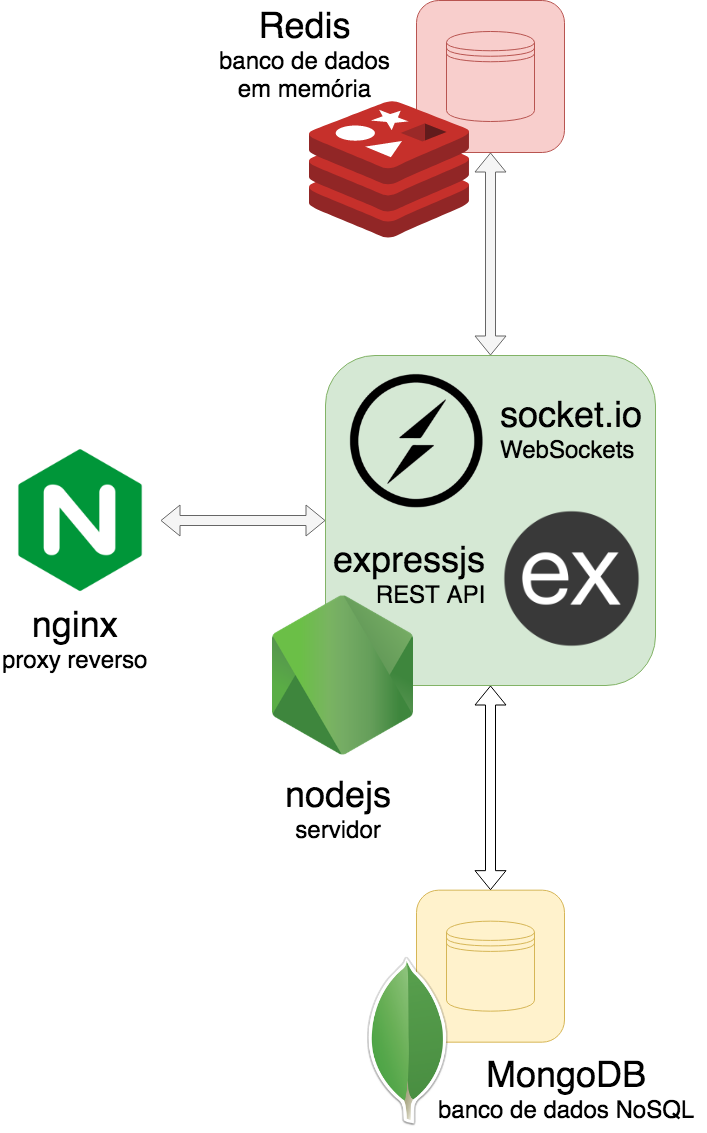
\includegraphics[width=0.5\textwidth]{componentesNuvem}
\label{fig:componentesNuvem}
\end{figure}

\subsection{Infraestrutura}

Para hospedar o servidor do Hedwig, foi utilizado o serviço de computação na nuvem Digital Ocean \footnote{https://www.digitalocean.com/}. Com ele, foi possível implantar o servidor em uma instância que roda Ubuntu 16.04.3 x64, com 1 CPU, 512MB de memória, 20GB de armazenamento de disco SSD e 1000GB de cota disponível para transferência de dados. O data center que hospeda essa instância fica em Nova Iorque.

\subsection{Segurança}

O servidor na nuvem suporta conexões HTTPS, permitindo que navegadores verifiquem a autenticidade do servidor e garantindo a privacidade e integridade dos dados transmitidos. Para isso, foi usado o Let's Encrypt\footnote{https://letsencrypt.org}, uma autoridade de certificação aberta, gratuita e automatizada. O Let's Encrypt usa o protocolo ACME (\emph{Automatic Certificate Management Environment}) para automatizar a comunicação entre autoridade e candidato para assegurar a autenticidade deste e conceder-lhe certificados de forma rápida e prática. É realizado um teste para verificar que o candidato possui controle sobre o domínio e, então, é gerado um certificado válido por 90 dias que pode ser renovado a qualquer momento. Para usá-lo no servidor, basta acrescentar novas configurações ao nginx.

Além disso, outra medida de segurança foi usar um \emph{firewall} para bloquear conexões nas portas TCP que não estão sendo usadas.

\subsection{Operação}

O serviço Keymetrics\footnote{https://keymetrics.io/} permite verificar se o servidor na nuvem está online, monitorar o uso de CPU e de memória, investigar a ocorrência de erros e realizar ações comuns, como reiniciar o processo do servidor, por meio de uma interface amigável. Investir em um sistema de monitoramento como esse auxilia tanto a manutenção preventiva como a corretiva, o que é essencial para um sistema de casa inteligente que tem a disponibilidade como requisito prioritário.

\begin{figure}[H]
	\centering
	\caption{Monitoramento do servidor na nuvem}
  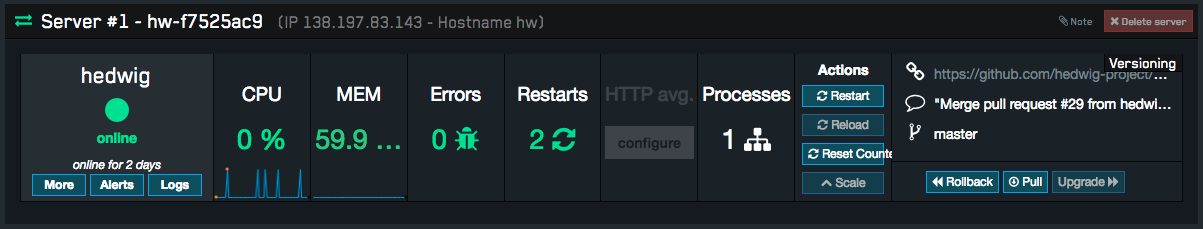
\includegraphics[width=1.0\textwidth]{keymetrics}
\label{fig:keymetrics}
\end{figure}

Outro ponto abordado é o uso de logs, arquivos que gravam eventos relevantes que acontecem no sistema. Eles podem ser usados para realizar a auditoria de falhas ocorridas e compreender melhor o funcionamento de um programa. Por questões de simplicidade, para classificar os eventos, o servidor na nuvem do Hedwig usa três do sete níveis de severidade definidos pelo padrão syslog \cite{rfc5424}: \emph{error}, \emph{warning} e \emph{informational}. O servidor implementa um esquema de rotação de logs, criando arquivos individuais para cada dia, o que facilita o arquivamento de logs muito antigos e a pesquisa de eventos específicos. Com esse sistema, também é possível filtrar eventos de severidades diferentes em arquivos separados.

\section{Aplicativo de dashboard}

\subsection{Descrição}
O aplicativo desenvolvido é uma dashboard que permite ao morador da casa ver os dados dos sensores em tempo real, enviar requisições para os módulos realizarem alguma ação, receber confirmações de que essas ações foram realizadas e gerenciar seus dispositivos - Morpheus e módulos. Essa dashboard foi implementada com base nas características dos PWAs apresentadas no capítulo de Arquitetura a fim de permitir uma boa experiência de usuário tanto em smartphones como em computadores.

\subsection{Requisitos}

\subsubsection{Requisitos funcionais}
\begin{description}

\item \textbf{Realizar cadastro, login e gerenciamento de informações pessoais}

\begin{itemize}
\item O usuário pode se cadastrar com seu email, nome e data de nascimento, criando também um nome de usuário e senha para acessar a dashboard.
\item O usuário pode realizar login usando seu nome de usuário e senha.
\item O usuário pode alterar as informações pessoais de seu cadastro.
\end{itemize}

\item \textbf{Gerenciar Morpheus}

\begin{itemize}
\item O usuário pode adicionar e remover controladores locais - Morpheus, sendo que para o cadastro basta adicionar o número de série do dispositivo.
\item O usuário pode configurar o Morpheus, especificando se deseja que mensagens que não puderam ser enviadas por problemas de conectividade sejam mandadas assim que a conexão for reestabelecida.
\end{itemize}

\item \textbf{Gerenciar módulos}

\begin{itemize}
\item O usuário pode adicionar e remover módulos, sendo que para o cadastro deve-se adicionar o número de série do dispositivo, relacioná-lo ao Morpheus que ouvirá suas mensagens, dar um nome ao módulo e seus relês e especificar o seu tipo.
\item O usuário pode configurar o módulo, especificando as configurações de conectividade, display e teste de auto-reset.
\end{itemize}

\item \textbf{Receber dados e enviar ações em tempo real}

\begin{itemize}
\item O usuário pode visualizar em tempo real os dados dos sensores de abertura, presença, temperatura, umidade e luminosidade do módulo básico.
\item O usuário pode visualizar o estado dos relês e enviar ações para ligá-los e desligá-los.
\item O usuário pode visualizar em tempo real os dados do estado do portão e do alarme do módulo de acesso.
\item O usuário pode, no módulo de acesso, enviar uma ação para abrir o portão usando uma senha.
\end{itemize}

\item \textbf{Alterar configurações avançadas dos módulos}

\begin{itemize}
\item O usuário pode receber confirmações de que ações sensíveis foram recebidas pelos módulos corretamente.
\item O usuário pode gerenciar o sensor de radiofrequência.
\item O usuário pode enviar uma ação para sincronizar a hora do módulo.
\item O usuário pode enviar uma ação para reiniciar o módulo (\textit{soft reset}).
\end{itemize}

\item \textbf{Visualizar estado das conexões}

\begin{itemize}
\item O usuário pode ver o status de sua conexão com o servidor da nuvem e da conexão de seus Morpheus com a nuvem.
\end{itemize}

\end{description}

\subsubsection{Requisitos não-funcionais}

\begin{itemize}
\item O aplicativo deve ser responsivo e totalmente funcional nos navegadores mais recentes em suas versões desktop e mobile.
\end{itemize}

\subsection{Tecnologias utilizadas}

Para criar a aplicação web que demonstra a funcionamento do Hedwig, foi escolhido o React\footnote{https://reactjs.org/}, biblioteca open source de JavaScript mantida pelo Facebook. O React é conhecido por facilitar o desenvolvimento de aplicações \textit{single-page}, renderizadas do lado do cliente, que permitem a atualização dinâmica da página de forma fluida e rápida, o que acaba enriquecendo a experiência do usuário. Possui uma linguagem declarativa e baseada em componentes, tornando-a altamente modularizável e reutilizável. Uma de suas características mais reconhecidas é o uso de um DOM virtual e um algoritmo de reconciliação que consegue identificar quais as partes da página que precisam ser renderizadas a cada interação com o usuário \cite{reactdiff}, melhorando a performance e permitindo maior fluidez em animações e mudanças visuais.

Outro ponto interessante para a utilização do React é que, com a biblioteca React Native\footnote{https://facebook.github.io/react-native/} - uma extensão do React - é possível a geração de aplicativos nativos para iOS e Android. Assim, caso surja a necessidade de implementar uma nova funcionalidade que possua algum requisito que não pode ser contemplado por um \textit{Progressive Web App}, mas pode ser atendido por um aplicativo nativo, pode-se usar o React Native. Isso diminui a necessidade de retrabalho e dispensa a necessidade de estudo aprofundado das linguagens e ambientes de desenvolvimento tradicionais de projeto de aplicativos nativos.

A fim de facilitar a implementação das interações com o usuário, usamos juntamente ao React a biblioteca Redux\footnote{https://redux.js.org/}, um gerenciador de estado global. Dessa forma, pretendemos facilitar o compartilhamento de informações entres diferentes componentes. A motivação por trás do Redux é facilitar a leitura e atualização do estado da aplicação, que, em sites \textit{single-page} modernos, pode armazenar respostas do servidor, cache de dados e dados criados localmente que ainda não foram persistidos no servidor. O Redux é baseado em três princípios \cite{redux}:

\begin{itemize}
\item O estado é o ponto único de verdade.
\item O estado permite apenas a leitura - a única forma de alterá-lo é emitindo uma \textit{action}.
\item Alterações no estado devem ser feitas por funções puras - são os chamados \textit{reducers}, que recebem o estado anterior e uma \textit{action} e retornam o novo estado.
\end{itemize}

\begin{figure}
	\centering
	\caption{Diagrama de funcionamento do Redux}
  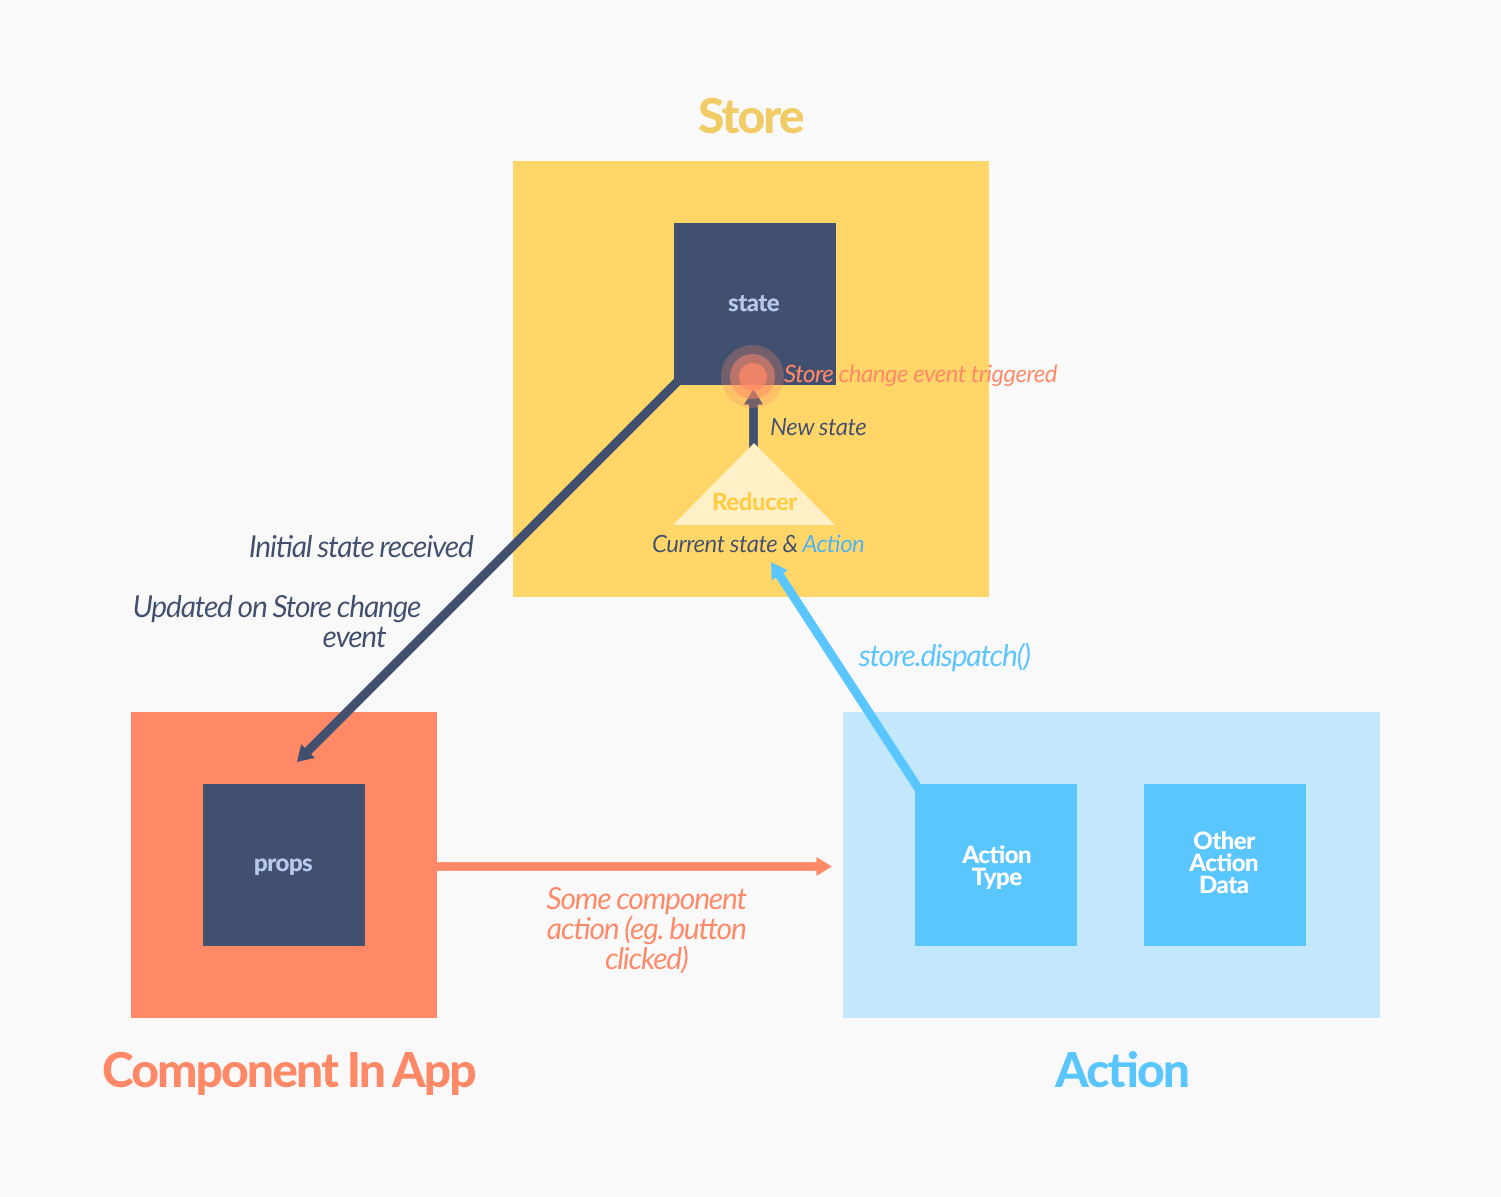
\includegraphics[width=\textwidth]{reduxFlowchart}
  \caption*{Fonte: \cite{reduxdataflow}}
\label{fig:reduxFlowchart}
\end{figure}

Para receber dados dos módulos em tempo real, foi usado um cliente do socket.io, framework que já foi discutido na seção do servidor na nuvem. O cliente de JavaScript já permite monitorar o status da conexão do aplicativo com o servidor, emitindo eventos em caso de desconexão ou reconexão. Assim, foi necessário criar \textit{listeners} para os eventos customizados que criamos para nossos protocolos.

Uma das vantagens em usar JavaScript para criar a view da aplicação é sua versatilidade, visto que é uma linguagem multi-paradigmas que suporta programação imperativa, declarativa e orientada a objetos \cite{mdnjs}. Outro ponto é que ela é usada tanto para desenvolvimento front-end como back-end, permitindo que o conhecimento acumulado na execução de um projeto ajude no outro.

Para aproveitar as funcionalidades e facilidades sintáticas das especificações mais recentes de JavaScript, usamos Babel\footnote{https://babeljs.io/}, um compilador capaz de converter as sintaxes novas e substituir as funções ainda não suportadas pelos navegadores com auxílio de \textit{polyfills}. Muitas vezes, é usado o termo transpilador para referir-se ao Babel, visto que é um compilador de JavaScript para JavaScript, não deixando de emitir como saída uma linguagem de alto-nível. Assim, é possível usar ES6 - a versãp mais recente de JavaScript - sem se preocupar com a compatibilidade do aplicativo com os navegadores que ainda não implementaram essa especificação completamente.

Para agilizar o desenvolvimento e prevenir falhas, usamos o \textit{linter} dedicado a JavaScript ESLint\footnote{https://eslint.org/}. \textit{Linter} é uma ferramenta para verificar o código e identificar erros de programação ou inconsistências de estilo \cite{linter}, o que possibilita produzir programas mais consistentes e menos suscetíveis a bugs.

Por fim, a pipeline de desenvolvimento do cliente usa o Webpack\footnote{https://webpack.js.org} como \textit{module bundler}. O Webpack cria gráficos de dependência de todos os componentes da aplicação web - imagens, folhas de estilo, scripts - e então os processa transformando-nos em \textit{bundles} ou pacotes, que nada mais são que arquivos estáticos.

\subsection{Interface}

\subsubsection{Identidade visual}

Para facilitar o desenvolvimento, foram usados os componentes do Material Design\footnote{https://material.io/} da Google, que satisfazem várias necessidades básicas e casos de uso da criação de interfaces modernas. Para distinguir cada tipo de módulo, foram usados ícones e paletas de cores distintas.

\subsection{Interações}

\subsubsection{Dados}

Dados provenientes dos sensores dos módulos são atualizados em tempo real por meio de eventos do socket.io. Para situar o usuário, o instante de tempo em que a mensagem do módulo foi enviada fica visível no fim na página. Caso seja detectado que a conexão com o Morpheus se perdeu, isso é mostrado explicitamente pela dashboard a fim de evitar que o usuário olhe dados antigos demais.

\subsubsection{Ações}

Ao enviar uma ação, o estado local do aplicativo não muda até que seja recebida uma nova mensagem de dados ou de confirmação. Isto é, se um relê está ligado e o usuário pede para desligá-lo, o aplicativo só vai mostrar que o relê desligou quando o módulo o avisa disso. Isso evita que o aplicativo entre em estados inconsistentes com os módulos.

\subsubsection{Conectividade}

O aplicativo possui um indicador no canto superior direito indicando o status da conexão. Ele pode assumir três estados:

\begin{itemize}
\item Aplicativos e todos os Morpheus do usuário estão devidamente conectados ao servidor na nuvem
\item Aplicativo está devidamente conectado ao servidor na nuvem, mas pelo menos um dos Morpheus não
\item Aplicativo não está conectado ao servidor na nuvem
\end{itemize}

Além disso, caso o aplicativo perca conexão com a nuvem, são emitidas notificações na parte inferior da tela. São realizadas 10 tentativas de reconexão e o resultado - positivo ou não - também aparece como um alerta na tela. Caso não haja sucesso em nenhuma das 10 tentativas, o usuário é aconselhado a atualizar a página.

\subsubsection{Aplicativo na tela inicial do dispositivo móvel}

Usando um arquivo de manifesto, foi possível configurar como o aplicativo aparece na tela inicial de um dispositivo móvel como um smartphone. Diminuindo o número de passos para o usuário acessar o aplicativo o encoraja a usá-lo mais vezes, além de criar uma sensação parecida com a de um aplicativo nativo.

\subsection{Publicação}

O aplicativo foi publicado com o serviço Surge\footnote{https://surge.sh/}, que permite a hospedagem de websites estáticos e oferece um domínio customizado. O Surge possui uma aplicação de linha de comando que permite a publicação de um diretório de arquivos HTML, CSS e JavaScript de maneira rápida e sem extensiva configuração. A dashboard está disponível em \url{https://hedwig.surge.sh}.

\subsection{Segurança}

O Surge usa a comunicação via HTTPS por padrão, oferecendo o suporte básico a SSL. Dessa forma, os dados transmitidos entre navegador e servidor podem ser criptografados, permitindo uma maior segurança em operações como cadastro, login e recebimento dos dados dos sensores.

\section{Aplicativo Backup}

Para lidar com o caso de indisponibilidade do controlador local Morpheus, da rede local (roteador wireless) ou da conexão com a Internet, foi desenvolvido um aplicativo de \textit{backup}. Esse aplicativo permite acesso direto ao módulo, através do endereço local (supondo que o dispositivo celular esteja na mesma rede) ou por conexão direta com o ponto de acesso do módulo (disponível todo o tempo, ou sempre que o módulo não consiga conexão com a internet, a depender da preferência do usuário).

\subsection{Requisitos}

Destacam-se os requisitos mais críticos do aplicativo backup:

\begin{enumerate}
	\item Permitir acesso direto ao módulo em caso de indisponibilidade da rede wifi e internet;
	\item Visualização de estado de sensores, e permitir a atuação em tempo próximo ao apresentado por botão físico;
	\item Acesso local, por meio de endereço local, ao módulo, no caso de haver rede local disponível, mas sem acesso à internet;
	\item Possibilitar ao usuário configurar rede WiFi, nome do módulo, cor do painel, offset de sensores, nome dos reles e regras de atuação (por rádio frequência, com senha ou não, por horário, por eventos dos sensores de presença e abertura,e tempo em que deve ficar ligado no caso de configurações automáticas);
	\item Permitir configurar códigos RF (rádio frequência) múltiplos para sensor de abertura, atuação do relé 1 ou do relé 2;
	\item Permitir ao usuário configurar controle de acesso e senha para atuação de um relé em específico;
	\item Segregar permissões entre administrador e usuário (usuários não podem executar configurações, somente visualizar estados e atuar em relés sem senha)
	\item Permitir visualização de vários módulos da residência;
	\item Ter interface de fácil navegação, intuitiva.
\end{enumerate}

\subsection{Tecnologias usadas}

Para o desenvolvimento do aplicativo backup, foram utilizados:

\begin{enumerate}
	\item Módulo como servidor, utilizando bibliotecas de comunicação próprias do ESP8266, no caso de comunicação direta com o módulo, e uso do módulo como cliente, usando a mesma biblioteca;
	\item Uso de ping para verificação de conexões e execução de rotinas para a correta configuração de estado do ponto de acesso (ligado se não conectado à rede), rotinas de desconexão e reconexão;
	\item CSS para a implementação de interface amigável para o usuário, e segregação de configurações em níveis de navegação maiores para que configurações mais usadas sejam mais facilmente acessíveis a partir do menu principal do módulo;
	\item Javascript para as rotinas de configuração e atualização do estado no menu principal;
	\item HTML4 para o desenvolvimento da maioria das páginas;
	\item EEPROM do módulo ESP8266, onde todas configurações de conexão, gerais e relés ficam armazenadas. Em caso de mudança desses parâmetros, ocorre sua persistência na EEPROM;
	\item Bibliotecas próprias para interface com sensores e outros periféricos (DHT, I2C, por exemplo), comunicação em geral, além do WiFi e Access Point (PubSub para comunicação por MQTT).
\end{enumerate}

\subsection{Navegação}

A partir da tela inicial, um cliente pode verificar todos os módulos presentes em sua casa, visualizar temperatura, umidade, luminosidade, sensores de presença ou abertura e apagar ou acender luzes (para atuadores protegidos com senha, o usuário deve acessar a página do respectivo módulo), numa interface configurável (o usuário pode configurar quais parâmetros observar nesse menu principal). A exibição da Figura \ref{fig:telasPrincipaisBackup} é própria para celulares, enquanto a exibição da Figura \ref{fig:plantaBackup}, com posicionamento configurável, simula a planta de uma casa (num cenário real, poderia ser a própria planta da casa do usuário), e é própria para desktops.

\begin{figure}[H]
	\centering
	\caption{Telas principais do Aplicativo Backup}
  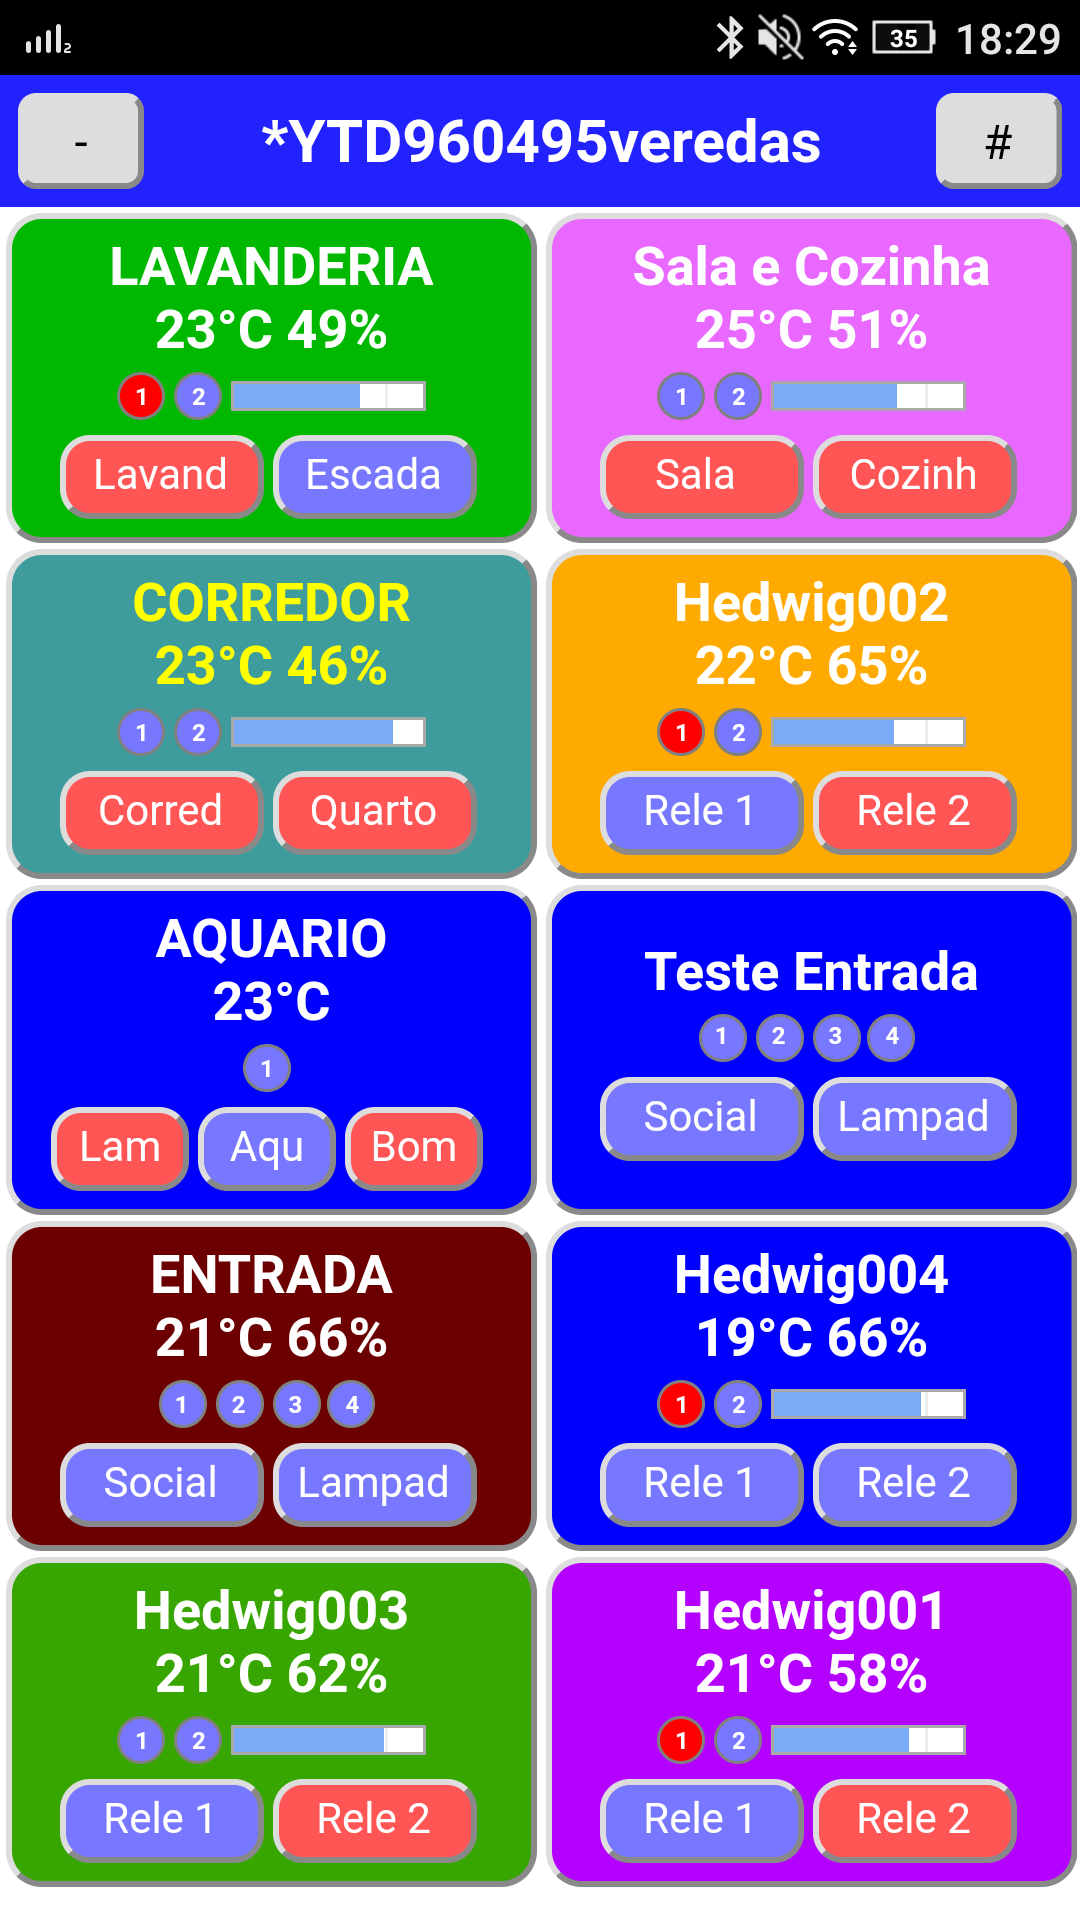
\includegraphics[width=0.5\textwidth]{telasPrincipaisBackup}
\label{fig:telasPrincipaisBackup}
\end{figure}

\begin{figure}[H]
  \centering
  \caption{Visão geral da planta de uma casa com o Aplicativo Backup}
  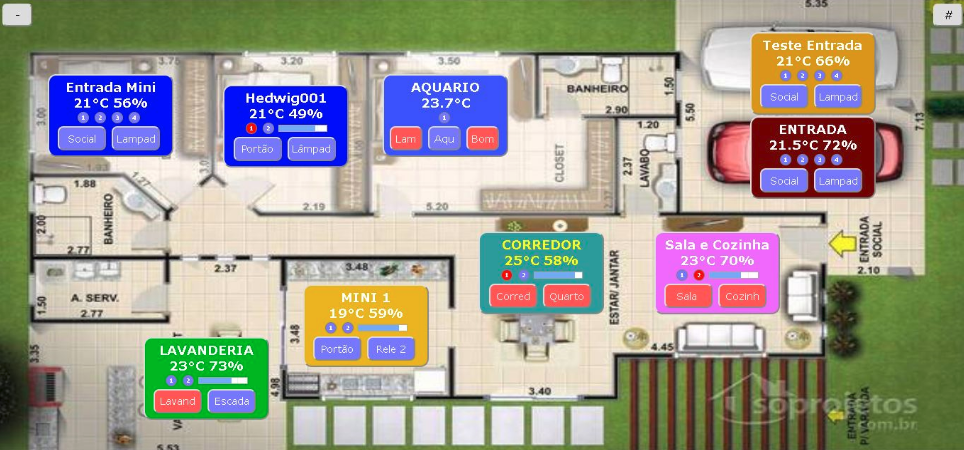
\includegraphics[width=0.8\textwidth]{plantaBackup}
  \label{fig:plantaBackup}
\end{figure}

A partir do menu principal, podemos acessar o menu do módulo desejado (vide Figura \ref{fig:menuPrincipalBackup}). Nele, encontram-se informações de luminosidade, horário, data, temperatura, umidade, sensor de presença (sensor 1) e sensor de abertura (sensor 2), além de controle de portão,lâmpada ou eletrodoméstico. Também exibe o nível de WiFi do módulo e a versão do firmware.

\begin{figure}[hbp]
    \centering
    \begin{minipage}{.4\linewidth}
        \centering
        \captionof{figure}{Menu principal do Aplicativo Backup}
        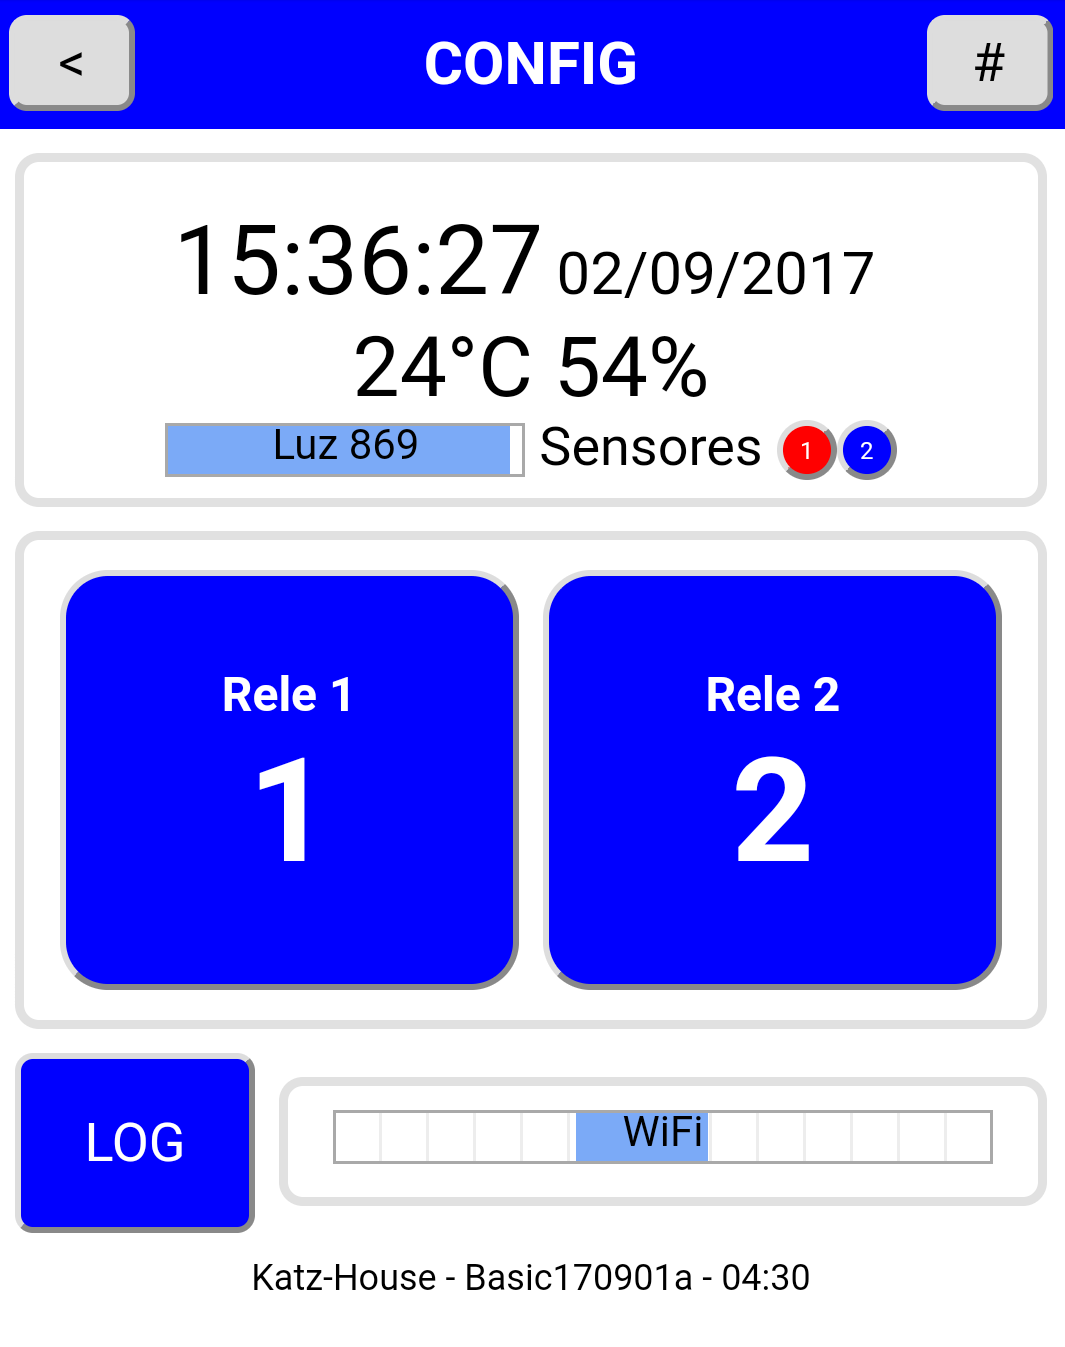
\includegraphics[height=6cm]{menuPrincipalBackup}
        \label{fig:menuPrincipalBackup}
    \end{minipage}
    \hfill
    \begin{minipage}{.4\linewidth}
        \centering
        \captionof{figure}{Teclado para digitação da senha}
        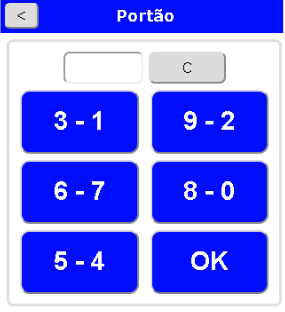
\includegraphics[height=6cm]{senhaBackup}
        \label{fig:senhaBackup}
    \end{minipage}
\end{figure}

No caso de proteção de controle por senha, é exibido o painel numérico como na Figura \ref{fig:senhaBackup}. A cada requisição da página, o modulo manda um mapeamento das teclas diferente (por exemplo, de teclas A,B,C,... para (3,1), (9,2), ...). Após o usuário entrar com a senha (sequência de teclas do tipo A, B, C, …), o módulo valida a sequência e autoriza o acionamento. Dessa forma, pessoas não conseguem copiar a senha ao visualizar a sequência de teclas do usuário, tampouco um invasor poderia copiar a sequência e utilizá-la para abertura logo em seguida, pois o mapeamento seria outro.

\subsection{Configurações}

A partir do menu principal do módulo, pode-se ter acesso ao seu log (para depuração, opção apenas para administradores) e um menu de configurações. Do menu de configurações, pode-se alterar o modo do display (dentre 3 opções), e as cores do módulo, conforme opções anteriormente citadas.

Ainda do menu de configurações, pode-se configurar alertas e alarmes (sonoros a partir dos módulos, e pela internet através do provedor gratuito Blynk e e-mail), relés (possibilidade de auto ligar a partir de um sensor específico, ou de ser acionado a partir de um sinal de rádio - usualmente um controle remoto ou até um sensor de abertura adicional, ou mais de um), e o log (quais parâmetros serão persistidos e mandados para a nuvem). Também pode-se acessar o menu de Ferramentas, onde é possível realizar testes de auto reset (para verificação do funcionamento do circuito antitravamento, que age em cerca de 30 segundos), reiniciar o módulo, desconectá-lo, voltar à versão de fábrica (versão implementada em software, enquanto a versão em hardware é realizada por meio de botão oculto), e atualizar o firmware (apenas disponível para administradores).
Ao acessar a atualização de firmware, escolhe-se a opção, que mostra a versão atual e, após escolha do arquivo, a versão a ser inserida.

É possível, também, acessar as configurações avançadas \ref{fig:firmwareconfigavancadasDHT}. Nela, podemos configurar um offset para temperatura e umidade (de preferência realizados a partir de um medidor confiável para calibração).

Do menu de configurações avançadas, podemos configurar os sensores e controladores de radio frequência (sem fio), aspectos de conectividade do servidor gratuito Blynk e possivelmente trocar a rede WiFi em que o módulo está conectado. Ainda, para administradores, há a opção de configurar os usuários que têm acesso ao módulo.

Ainda pode-se trocar o nome do módulo, e ativar/desativar o ponto de acesso (para acesso direto ao módulo), além de configurar o nome (SSID) e senha de sua rede WiFi.

Demais ilustrações, referentes às configurações, estão disponíveis no Anexo \ref{attachmentsImagensBackup}{}.

\subsection{Abertura de porta do roteador}

Para acessar o módulo/menu remotamente, podemos usar a abertura de porta (NAT/virtual servers), configurável nas páginas de configuração dos roteadores. Maiores informações para essa configuração podem ser encontradas nos manuais dos roteadores. (Observe que há uma segurança menor envolvida com essa configuração). Há a abertura da porta para acesso remoto sem a necessidade de serviços em nuvem, para usuários que podem lidar com um nível de segurança mais baixo.

\begin{figure}[hbp]
    \centering
    \caption{Página de configuração TP Link}
    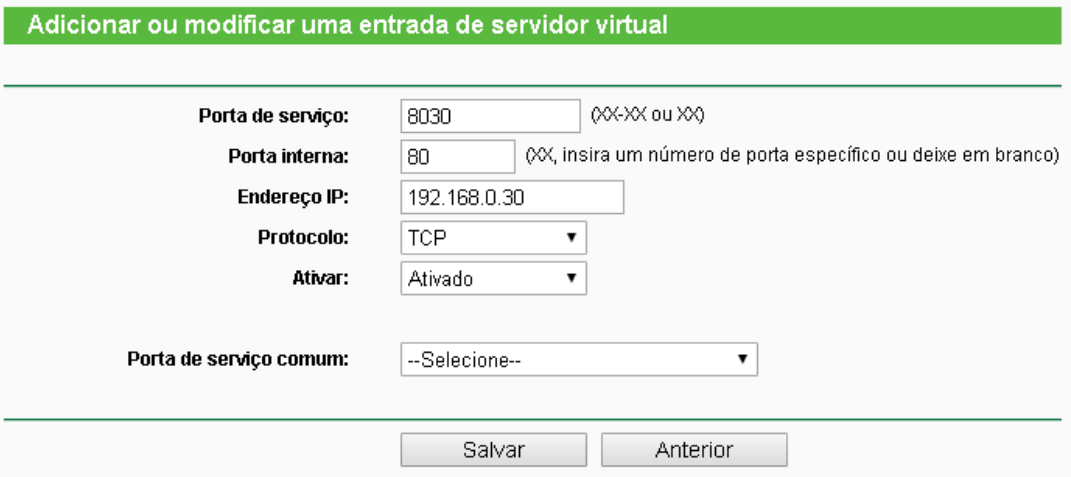
\includegraphics[width=0.8\textwidth]{tpLinkAppBackup}
    \label{fig:tpLinkAppBackup}
\end{figure}

\emph{Obs.:} Caso sua operadora só forneça o CGNAT, a abertura de porta por parte do usuário não será possível.

\subsection{Controle remoto}

Para que o controle remoto seja corretamente configurado, são necessários os seguintes passos.
\begin{enumerate}
    \item
    A partir da página inicial do módulo, entre em \# \textrightarrow{} Configurações Avançadas \textrightarrow{} RF433

    \item
    Configure o Sensor de Abertura “Sulton” no modo 2, para mandar sinais diferentes de abertura e fechamento. Consulte o manual do fabricante.

    \item
    Aperte +, espere até a página indicar “Aguardando”, e abra o sensor de abertura. (Podemos incluir diversos sinais para o controle do mesmo relé, abertura ou fechamento de sensor). Aperte “OK” no canto superior direito da página, para salvar suas configurações.

    \item
    Repita o passo 3 para o fechamento do sensor de abertura. \textbf{Cuidado:} O sensor de abertura repete algumas vezes o mesmo sinal. Aguarde alguns instantes entre gravar a abertura e o fechamento para não gravar o mesmo sinal (isso pode ser verificado na série numérica que aparece gravada. Se estiver igual, temos um problema).

    \item
        \begin{enumerate}
            \item
            A partir da página inicial do módulo, entre em \# \textrightarrow{} Configurações Avançadas \textrightarrow{} RF433.

            \item
            Aperte + (ao lado do rele 1 ou rele 2), espere até a página indicar “Aguardando”, e abra o sensor de abertura. (Podemos incluir diversos sinais para o controle do mesmo relé, abertura ou fechamento de sensor).

            \item
            Aperte "OK" no canto superior direito da página, para salvar suas configurações.

        \end{enumerate}
\end{enumerate}

\subsection{Notificações}
Para que as notificações sejam ativadas, utilize os próximos passos.

\begin{enumerate}
    \item
    Para que o suporte consiga acessar remotamente o módulo e realize a coleta de dados, acesse \# \textrightarrow{} Configurações Avançadas.\textrightarrow{} Blynk

    \item
    Insira o Auth Token (e.g. aa7a6dc1170640f08e951ed8cd2198a1).

    \item
    Selecione Notificações ao iniciar: Sim, e WiFi: Sim.

    \item
    Aperte em OK, no canto superior direito, para salvar suas alterações.
\end{enumerate}

\subsection{Offset de temperatura e umidade}

\begin{enumerate}
    \item
    Para que o suporte consiga acessar remotamente o módulo e realize a coleta de dados, acesse \# \textrightarrow{} Configurações Avançadas.\textrightarrow{} Temperatura e Umidade.

    \item
    Efetue a calibração do equipamento usando uma referência externa.

    \item
    Aperte em OK, no canto superior direito, para salvar suas alterações.
\end{enumerate}

\subsection{\emph{Hard reset}}
\begin{enumerate}
	\item Ligue na tomada
	\item Abra a tampa do módulo, e retire o isopor que cobre o sensor de temperatura azul;
	\item Localize o botão (“pushbutton”), após retirar o isopor;
	\item Pressione o botão até ouvir 6 beeps;
	\item O módulo retornará para a configuração de fábrica. Veja as seções a seguir para sua configuração inicial.
\end{enumerate}

\subsection{Setup inicial}
\begin{enumerate}
	\item Primeiro, conecte à rede Wifi do Módulo, com nome CONFIG (senha: A senha da rede CONFIG é 12345678)
	\item Abra um navegador e vá ao endereço 192.168.4.1 para entrar na página de configuração. Entre com as credenciais (login: admin e senha: 1234);
	\item Espere até que as redes disponíveis apareçam, selecione-a e forneça sua senha, para conectar o módulo à internet.
	\item Observe o endereço local 192.168.0.X que aparecerá no lcd do módulo. Caso não consiga ver, realize o passo 7 e use uma ferramenta como o “Zentri” (aplicativo Android) para descobrir em que endereço o módulo entrou. Para ver na tela novamente, pode tirar o módulo da tomada e ligá-lo novamente
	\item Espere o módulo reiniciar (continue na rede CONFIG), e aguarde até a página recarregar. Insira o nome do módulo e depois aperte “Salvar e Reiniciar”.
	\item Conecte-se novamente na rede WiFi da sua casa.
	\item Entre no endereço 192.168.0.X que foi mostrado no módulo, clique em \# e então em “Reiniciar Busca”, Aguarde até que todos os módulos sejam descobertos.
	\item Retorne para a página anterior (usando o “<” no canto superior esquerdo). Você verá o menu principal da casa, e daí poderá controlar reles, visualizar dados coletados pelos módulos e entrar em cada módulo. O menu é personalizado na página anterior (ao pressionar o “\#” no canto superior direito da tela).
\end{enumerate}

\section{Módulos}
\subsection {Rotinas}
\subsubsection{Multiplexação no tempo}
Para tratar indisponibilidade dos módulos devido a tentativas de reconexão e conexão e requisições não-gerenciadas, e, assim, aumentar a disponibilidade, existem além do circuito antitravamento e \textit{hard reset} diversas rotinas de tratamento. Elas contemplam desde configuração inicial, reconfigurações, coletas de dados e atuação por meio de relés até conexão, desconexão, reconexão e envio de dados. Elas foram multiplexadas no tempo da seguinte forma:

\begin{figure} [H]
	\centering
	\caption{Rotina de multiplexação de procedimentos no tempo}
  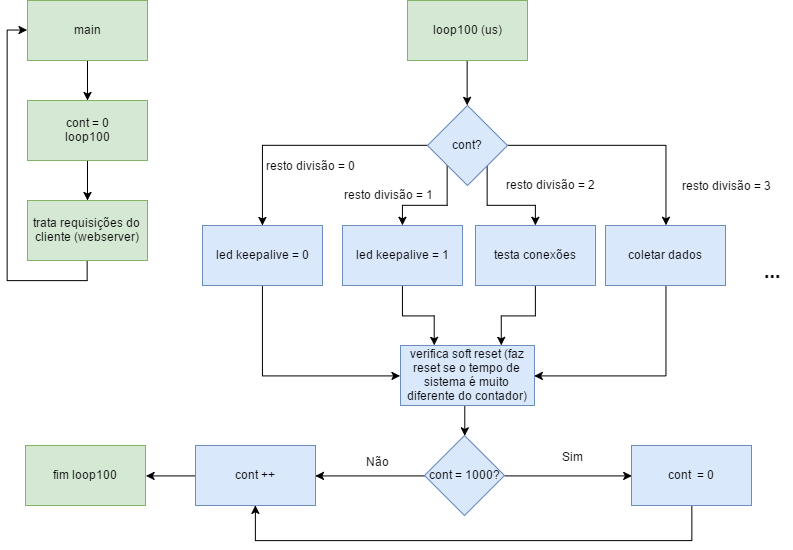
\includegraphics[width=0.8\textwidth]{rotinaMultiplexacao}
\label{fig:rotinaMultiplexacao}
\end{figure}

\subsubsection{Tratamento de indisponibilidade}
Nos casos de indisponibilidade de Internet, servidor ou rede local, o seguinte procedimento foi adotado (observe que a indisponibilidade do próprio módulo é tratada pelo circuito antitravamento):

\begin{figure}[H]
	\centering
	\caption{Tratamento de indisponibilidade de recursos}
  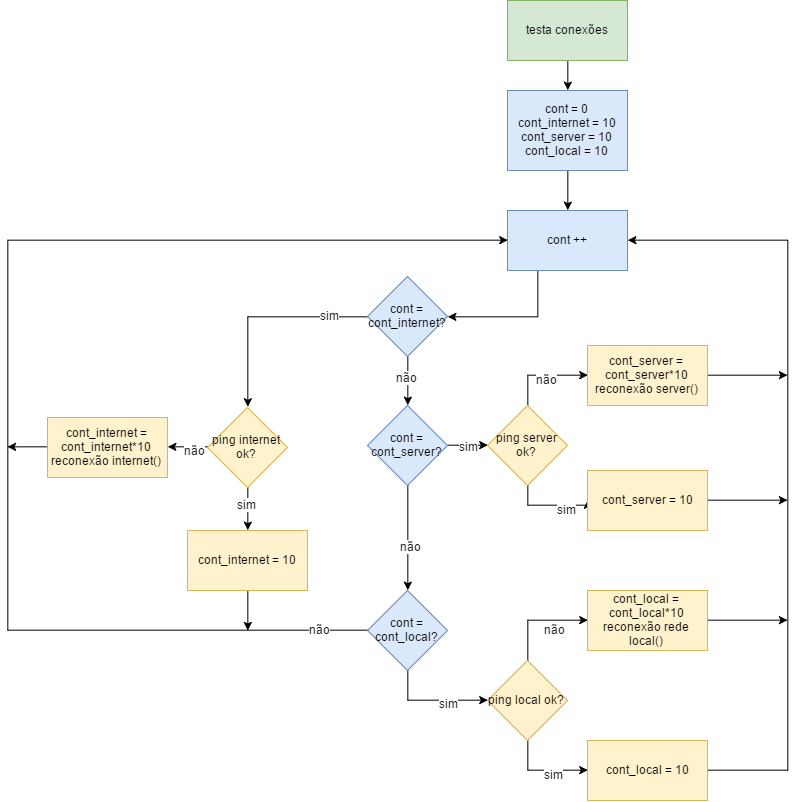
\includegraphics[width=0.8\textwidth]{tratamentoIndisponibilidade}
\label{fig:tratamentoIndisponibilidade}
\end{figure}

Com esse procedimento, as tentativas de reconexão à Internet, servidor e rede local estão segregadas e com tentativas realizadas em intervalos de tempo sucessivamente maiores. Desta forma, conseguimos gerenciar esses procedimentos, já que o nível de processamento é baixo.

\subsubsection{DoS local (\textit{Evil Twin})}
No caso de ataque de \textit{Evil Twin} - no qual uma rede mal-intencionada, usualmente aberta, usa o mesmo SSID da rede original com o objetivo de obter a senha - o sistema pode ficar indisponível até ao nível local. Módulos podem se conectar à rede mal-intencionada e ficarem somente com as funcionalidades offline, como acionamento de lâmpada por botão físico acoplado ao módulo. Outro problema é a queda da rede por interferência de radiofrequência ou outro mecanismo utilizado pelo usuário mal-intencionado para que os clientes se desconectem, tentem reconexão e forneçam a senha da rede.

Além do problema de indisponibilidade, no caso do dispositivo ser capturado pela rede mal-intencionada e ser controlado por usuários não legítimos, há a possibilidade dos módulos contribuírem para um ataque de \textit{DDoS} \cite{OVHDDoS}.

Para mitigar esses riscos, os módulos executam o seguinte procedimento:

\begin{figure}[H]
	\centering
	\caption{Tratamento de ataque de DoS Local}
  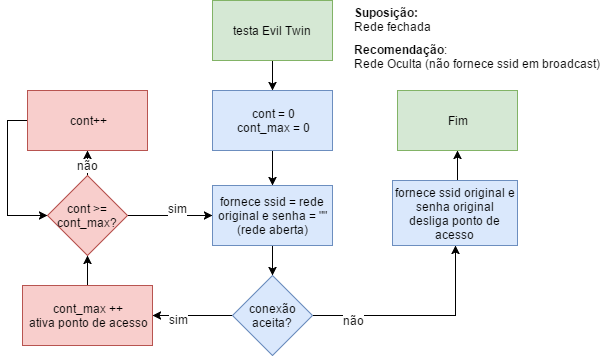
\includegraphics[width=0.8\textwidth]{tratamentoDoS}
\label{fig:tratamentoDoS}
\end{figure}

\subsubsection{Comunicação por MQTT}
Para o desenvolvimento da comunicação por MQTT com o Morpheus no módulo, foi usada a biblioteca PubSub para Arduino.

Para cada módulo existem identificador e senha, que são parâmetros próprios saídos de fábrica, além de configurações de porta e endereço do Morpheus local padrões.

O controle de comunicação foi realizado da seguinte forma:

\begin{enumerate}
	\item Só há tentativa de conexão MQTT em caso de haver conexão do Wi-Fi e o horário interno estar configurado --- caso contrário, pode-se provocar travamento do módulo ou envio de mensagens sem \emph{timestamp}.
	\item É executada configuração de \emph{callback} e de servidor MQTT a cada reconexão -- este ponto foi crítico para o bom funcionamento da comunicação.
	\item No \emph{callback} ocorre recebimento de mensagens e tratamento (\emph{parsing} da mensagem recebida, o que é feito por meio de obtenção de seu tipo e redirecionamento para rotinas específicas para obtenção dos parâmetros de interesse de cada mensagem).
	\item Envio de mensagens de estado a cada um minuto ou quando houver mudança brusca em um dos sensores (presença, abertura, umidade ou temperatura) ou então requisição de atuação; nesses casos de envio rápido, a mensagem é inserida no início da fila de saída e enviada logo em seguida, em até um segundo.
	\item Após o tratamento inicial das mensagens e a obtenção dos parâmetros de interesse, ocorre a persistência nas variáveis internas e gravação da EEPROM para que configurações e estados executados no aplicativo backup ou pela dashboard sejam refletidos dos dois lados, tornando transparente ao usuário o uso de qualquer um dos aplicativos e integrando suas funcionalidades.
	\item Ainda em fase final, após a persistência de variáveis na EEPROM, ocorre a inclusão na fila de saída de mensagens de confirmação para o servidor local.
	\item A fila de saída é usada para o envio periódico das mensagens de estado.
\end{enumerate}

\begin{figure}[H]
	\centering
	\caption{Exemplo de estado da fila de saída de mensagens MQTT do módulo}
	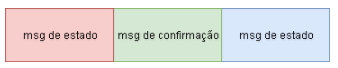
\includegraphics[width=0.5\textwidth]{filasaidaMQTT}
	\label{fig:filasaidaMQTT}
\end{figure}

Mensagens de estado periódicas (azuis) são inseridas no final da fila. No caso de acionamento, uma mensagem de estado (vermelha) é inserida no início da fila, e, em caso de configuração, uma mensagem de confirmação também é inserida no início da fila.

Por fim, vale destacar a necessidade de alteração da biblioteca PubSub para suportar mensagens maiores. Em caso de impossibilidade de envio de mensagens maiores, todo o protocolo deveria ser alterado para comportar mensagens mais compactas ou então deveria haver o uso de algum mecanismo de codificação ou compactação em conjunto com o protocolo desenvolvido.

\subsection{Diagrama}
Abaixo está o diagrama do circuito impresso (PCB).

\begin{figure}[H]
	\centering
	\caption{Diagrama PCB do Módulo Base}
  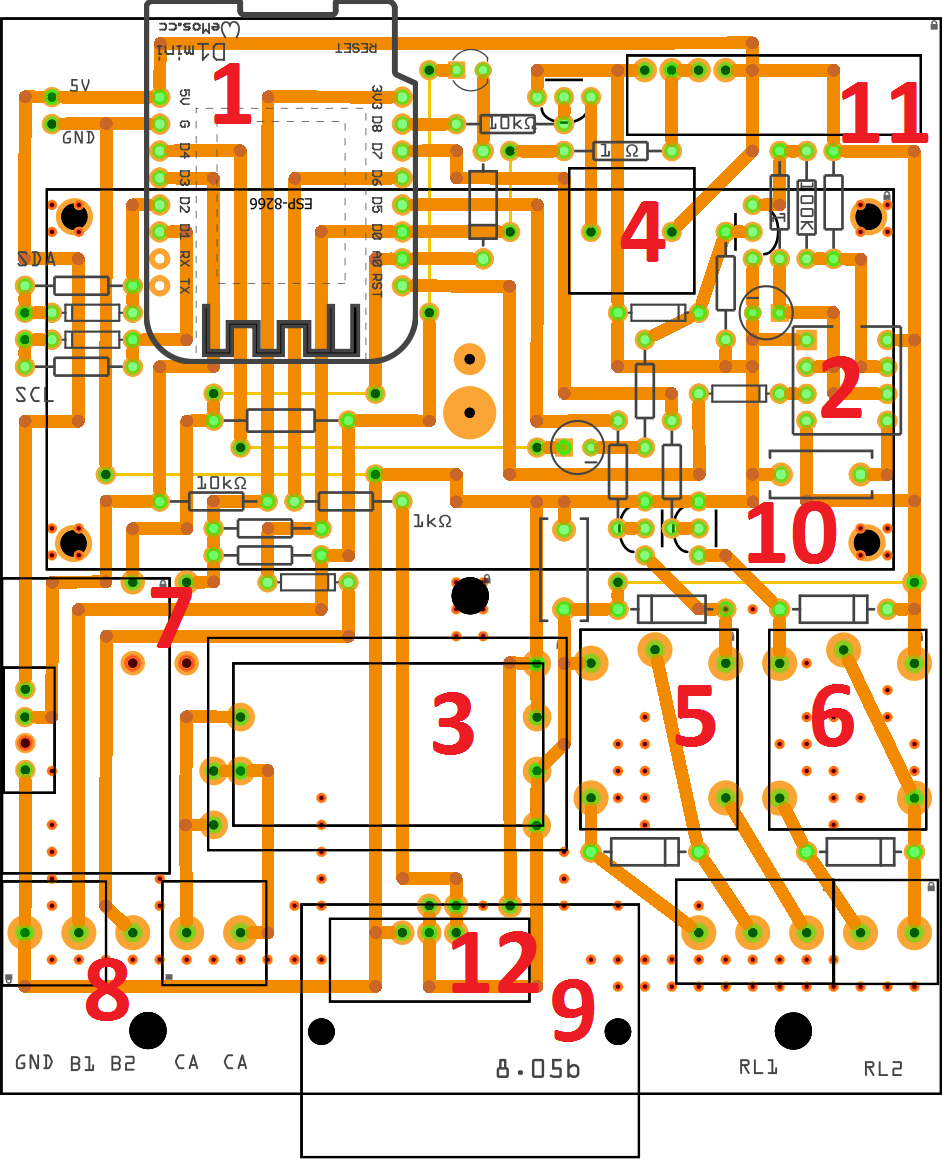
\includegraphics[width=0.8\textwidth]{diagramaModuloBase}
\label{fig:diagramaModuloBase}
\end{figure}

\begin{enumerate}
\item Wemos D1 mini
\item Astável 555
\item Fonte 5V 3W
\item \textit{Buzzer}
\item Relé 1
\item Relé 2
\item \emph{Hard reset}
\item Botões
\item Presença
\item RF-RX
\item RF-TX
\end{enumerate}

\begin{figure}[H]
	\centering
	\caption{Diagrama elétrico do Módulo Base}
  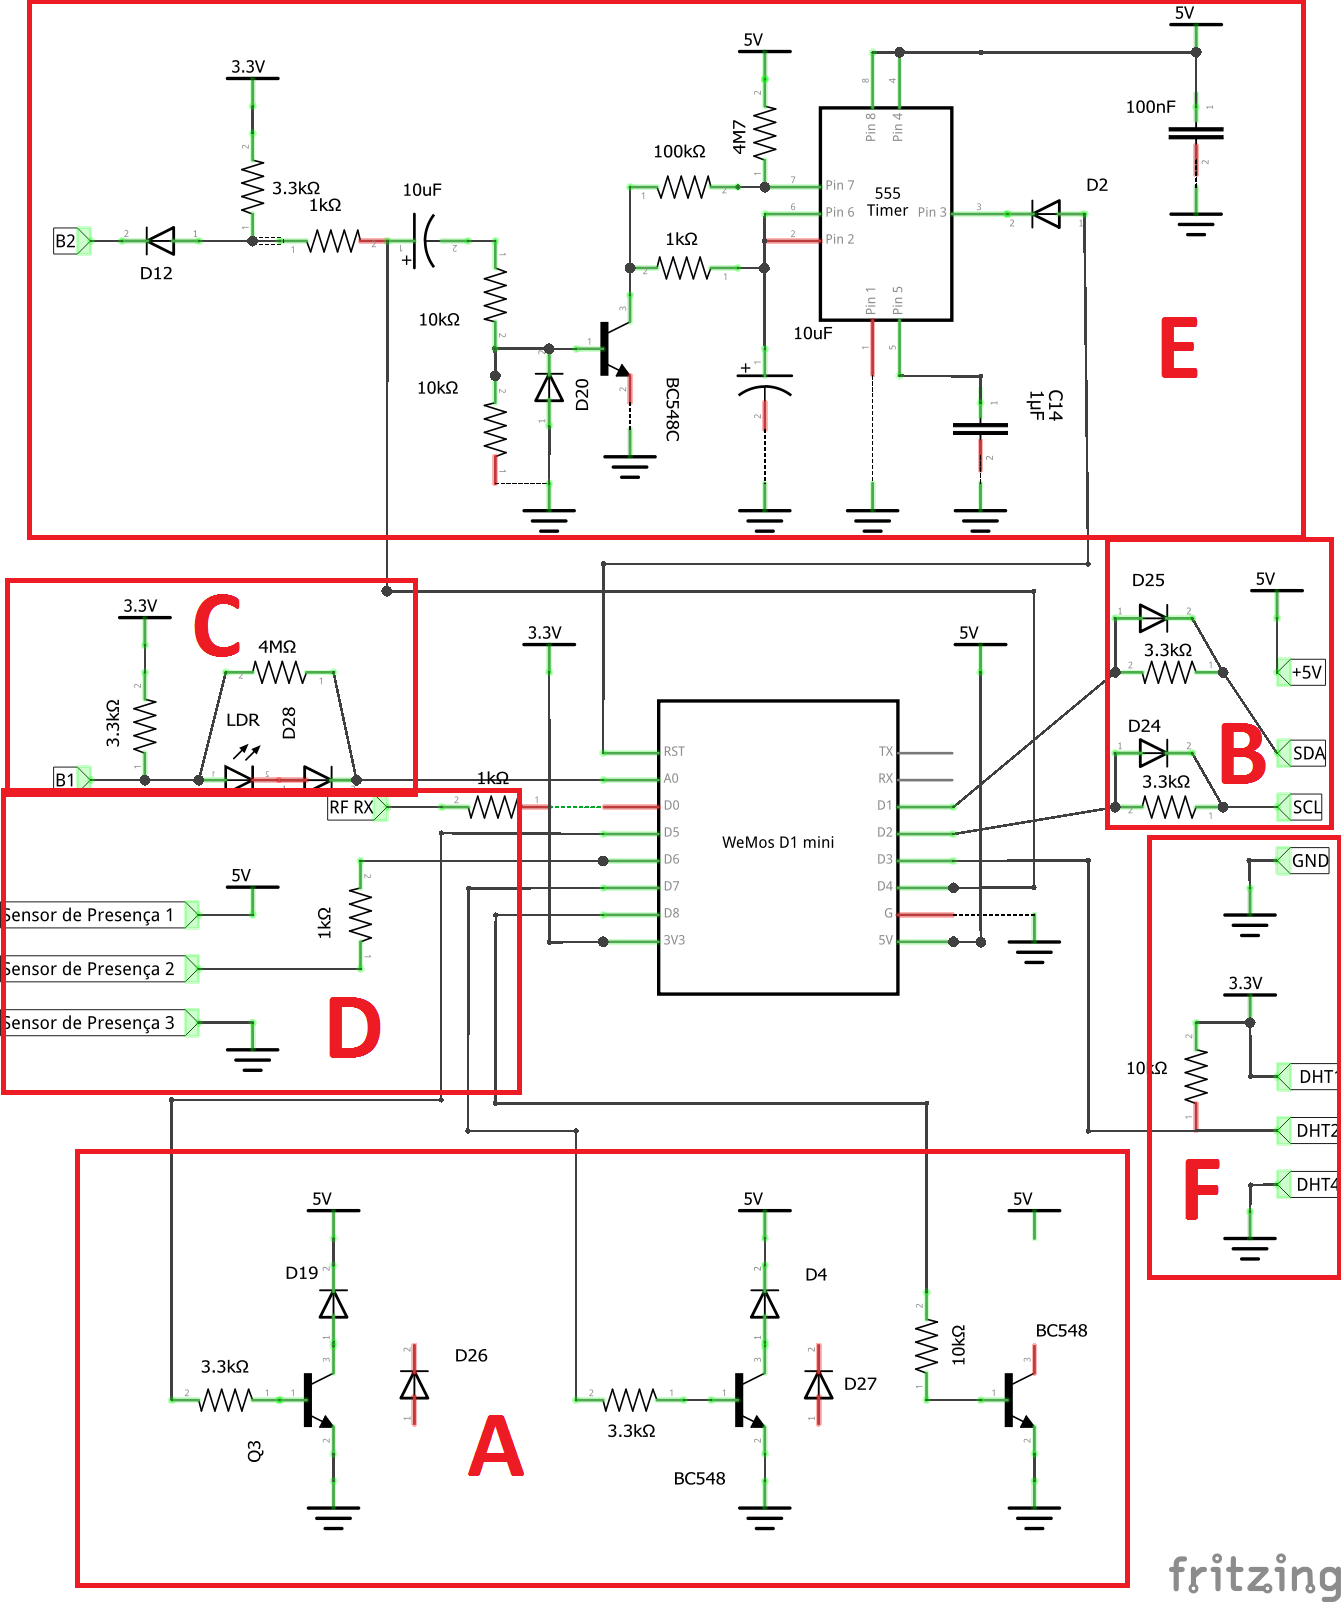
\includegraphics[width=0.8\textwidth]{esquematicoModuloBase}
\label{fig:esquematicoModuloBase}
\end{figure}

% TODO revisar as legendas desse cara, usar as letras da imagem?
\begin{description}
\item [A - Saídas] Circuitos simples de transistor para acionamento de relés (para lâmpadas) e \emph{buzzer}.
\item [Proteção 3V3 5V] Como o display trabalha com tensão de 5V, há proteções com diodos para não danificar as entradas digitais do Wemos D1 mini, que trabalha com tensão de 3V3.
\item [3 Entradas em A0] O circuito tem como entradas um botão (para acionamento do relé 1), o LDR (para chaveamento da luz de fundo do display) e um outro botão para \emph{hard reset} do dispositivo, todos em uma entrada analógica, cujo mapeamento E/S é da seguinte forma:

\begin{figure}[H]
	\centering
	\caption{Entradas em A0}
  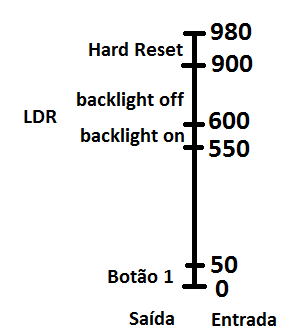
\includegraphics[width=0.4\textwidth]{entradasEmA0}
\label{fig:entradasEmA0}
\end{figure}

\item [Presença ou RF-TX] A entrada digital D6 é usada exclusivamente como entrada do sensor de presença PIR ou receptor RF.
\item [Astável 555 para \emph{hard reset} e Botão] A porta D6 é usada como LED \textit{keep alive} do módulo. Sua demora ao piscar indica que o módulo está travado ou demorando muito para processar algo, o que não deveria acontecer, uma vez que os procedimentos estão multiplexados no tempo de acordo com seus tempos limite. Dessa forma, essa saída está conectada a um circuito antitravamento, que executa o \emph{reset} nos casos mencionados, de travamento ou \textit{timeout}.

O primeiro capacitor tem como objetivo desacoplamento DC, de forma que a entrada do circuito envolvendo o astável 555 seja somente AC. Assim, permanências em 0 ou 1 indicam travamento.

Enquanto o LED pisca em intervalos esperados regularmente, o transistor conduz e mantém uma saída dente de serra muito próxima de 0. Quando o módulo trava, o transistor não conduz mais, e a saída passa a oscilar entre 1/3 e 2/3 da tensão total. Observe que o carregamento é feito pelo resistor de 4M7, muito maior que o resistor de 100k, fazendo com que o tempo de carga seja muito maior que o tempo de descarga, uma vez que esses tempos são diretamente proporcionais à constante de tempo dos circuitos RC, que é dada pelo produto do R*C. Durante a descarga, o \emph{reset} da placa é realizado. Observe que os tempos foram ajustados pelos valores dos componentes discretos, para que o tempo entre \emph{resets} sucessivos seja menor que o tempo necessário para o módulo voltar a funcionar após um \emph{reset}.

Segue abaixo uma ilustração sobre o funcionamento do circuito.

\begin{figure}[H]
	\centering
	\caption{Funcionamento do circuito antitravamento}
  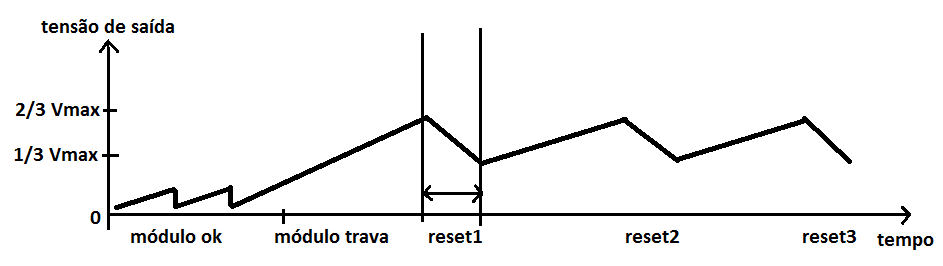
\includegraphics[width=0.8\textwidth]{circuitoAntiTravamento}
\label{fig:circuitoAntiTravamento}
\end{figure}

\item [DHT11] Entrada D3 é ligada a uma montagem básica para leitura de umidade e temperatura através do periférico DHT11.

\end{description}

\subsection {Montagem}

As fotos e comentários seguintes descrevem o processo de montagem física dos quatro módulos usados neste trabalho. Além destes, outras versões também foram construídas anteriormente no decorrer do projeto, instaladas na residência de um dos membros do grupo e usados para coleta de dados. Tais versões, por se tratarem de protótipos, não têm sua montagem completamente documentada, tampouco a uniformidade apresentada nos módulos seguintes.
Ao final, também consta o procedimento utilizado para validação dos módulos após sua construção, que contribuiu para a identificação de ligações não realizadas e outros problemas de montagem.

\begin{figure}[H]
	\centering
	\caption{Evolução do hardware (de fevereiro/17 a setembro/17)}
	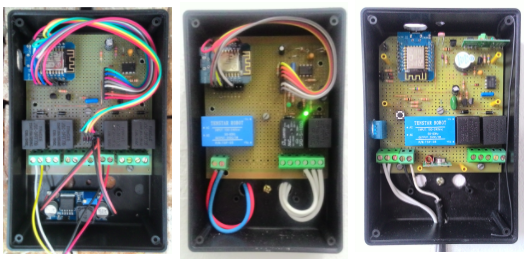
\includegraphics[width=0.8\textwidth]{evolHW}
	\label{fig:evolHW}
\end{figure}

\begin{figure}[H]
	\centering
	\caption{Evolução da caixa de proteção e display}
	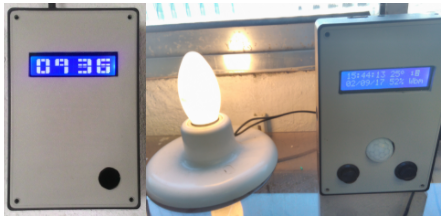
\includegraphics[width=0.8\textwidth]{evolProtDisplay}
	\label{fig:evolProtDisplay}
\end{figure}

\begin{figure}[H]
	\centering
	\caption{Materiais e preparação da placa padrão}
	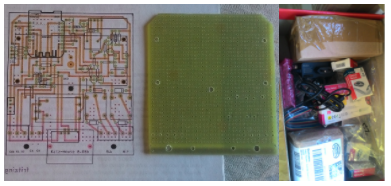
\includegraphics[width=0.8\textwidth]{materiaisPrepPlaca}
	\label{fig:materiaisPrepPlaca}
\end{figure}

\begin{enumerate}
	\item Primeiramente, a partir do esquemático em escala real, foram cortados e realizados furos na placa padrão.

	\begin{figure}[H]
		\centering
		\caption{Posicionamento dos componentes}
		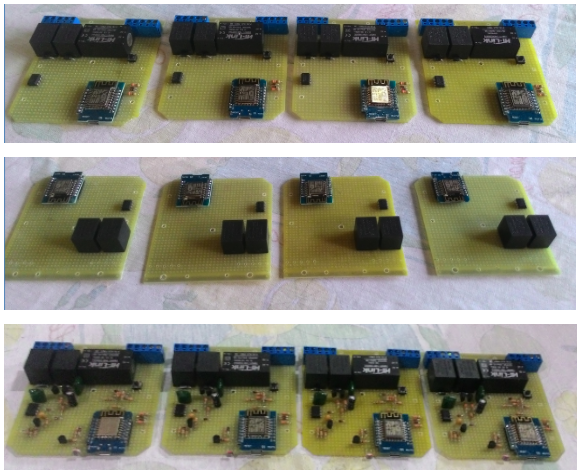
\includegraphics[width=0.8\textwidth]{PosicionamentoComp}
		\label{fig:PosicionamentoComp}
	\end{figure}

	\item Em seguida, foram posicionados os componentes.

	\begin{figure}[H]
		\centering
		\caption{Preparação dos displays com o I2C e soldagem}
		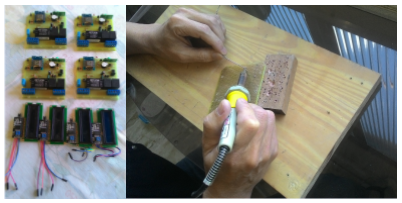
\includegraphics[width=0.8\textwidth]{PrepI2CSoldagem}
		\label{fig:PrepI2CSoldagem}
	\end{figure}

	\item A próxima etapa foi soldar as trilhas por baixo conforme o diagrama. Também foi necessário soldar o I2C com o display. Essa é a etapa mais demorada, que poderia ser facilmente operacionalizada ao serem adotadas placas de circuito impresso, o que aumentaria muito a capacidade de montagem.

	\begin{figure}[H]
		\centering
		\caption{Preparação das caixas para os módulos}
		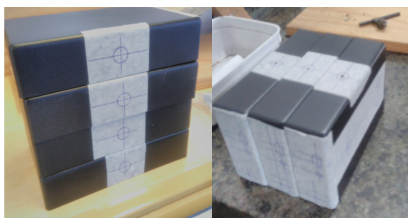
\includegraphics[width=0.8\textwidth]{PrepCaixasModulos}
		\label{fig:PrepCaixasModulos}
	\end{figure}

	\item Prossegue-se para a marcação das caixas para uso das furadeiras e lixas. Com ferramentas mais adequadas, essa etapa também poderia ser mais rápida e eficiente.

	\begin{figure}[H]
		\centering
		\caption{Caixa protetora, ligação dos botões e cabos de força}
		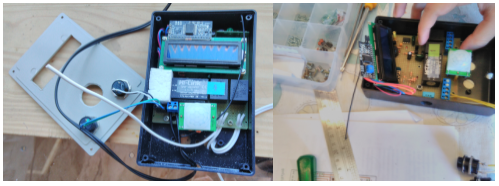
\includegraphics[width=0.8\textwidth]{BotoesCabosForca}
		\label{fig:BotoesCabosForca}
	\end{figure}

	\item Com a caixa preparada, foi possível inserir as placas padrão com os componentes e trilhas. Restou fixá-los com parafusos, montar a sustentação do display e sensor de presença (também integrado nesse passo), isopor para isolar termicamente o medidor de temperatura e umidade DHT, além de fazer as ligações dos botões, cabos de força e fios dos relés.

	\begin{figure}[H]
		\centering
		\caption{Quatro módulos prontos}
		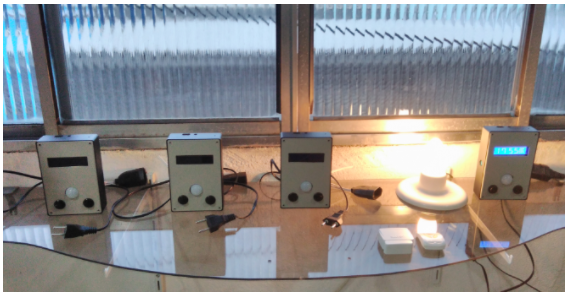
\includegraphics[width=0.8\textwidth]{QuatroModulos}
		\label{fig:QuatroModulos}
	\end{figure}

\end{enumerate}

\subsubsection {Montagem}
\begin{enumerate}
	\item Carregar programa para testar módulo;
	\item Realizar setup da conexão com a rede Wi-Fi;
	\item Verificar com o multímetro se há curto em algumas ligações principais (terra, VCC);
	\item Checar a alimentação da fonte e sua saída correta;
	\item Realizar o \emph{hard reset} ao apertar o botão atrás do isopor do DHT até ouvir 10 bipes;
	\item Fazer o passo 2 novamente, pois o módulo deve ter voltado à versão de fábrica. Logo em seguida, fazer o teste de \emph{auto reset}, que serve para verificar se o circuito antitravamento está funcionando. Para esse teste, é simulado uma pausa do sinal \emph{keep alive} que o circuito baseado no astável 555 monitora;
	\item Cobrir o sensor de presença. Verificar a inatividade no aplicativo. Descobrí-lo e verificar atividade;
	\item Executar o passo 7 para o sensor de luminosidade (LDR) também;
	\item Verificar com um medidor externo ou consulta a um site de previsões do tempo se as medidas de temperatura e umidade estão de acordo. Realizar ajuste (offset) no aplicativo se necessário;
	\item Verificar o funcionamento dos botões, acionando-os um por um;
	\item Checar o acionamento dos relés pelo aplicativo web também;
	\item Após gravar o RF de um controle para os dois relés, testar seu funcionamento;
	\item Verificar com um multímetro a saída dos relés (se troca de nível com acionamento pela página web, botões e controle RF).
\end{enumerate}


\chapter{Aprendizado de máquina}

	\section{Conceito}
		% TODO colocar referência ao curso do Andrew Ng
		O termo Aprendizado de Máquina (\emph{Machine Learning}) surgiu em 1959, sendo utilizado pela primeira vez  pelo cientista americano Arthur Samuel. O termo foi por ele definido como "o campo de estudos que dá a um computador a habilidade de aprender sem ser explicitamente programado" (tradução livre dos autores). Em 1998, Tom Mitchel - outro cientista da computação americano - propôs uma explicação menos abstrata do termo da seguinte maneira: "um programa de computador aprende com a experiência E com respeito a uma classe de tarefas T e medida de performance P se sua performace nas tarefas T, sendo medida por P, aumenta com o aumento da experiência E".

		% TODO colocar referencia https://hbr.org/2017/07/whats-driving-the-machine-learning-explosion
		Apesar do conceito de aprendizado de máquina existir desde a década de 50, seu crescimento e relevância aumentaram apenas na última decada. Alguns fatores levaram a esse crescimento acelerado. Os principais foram o aumento da quantidade de dados - e aplicações de \emph{IoT} têm propulsionado esse aumento - coletados e disponíveis, a melhora nos algoritmos, e o \emph{hardware} cada vez mais poderoso dos computadores. Esses últimos dois fatores permitem que a vasta quantidade de dados que possuímos possam ser analisados em tempo viável.

	\section{Relação com o projeto Hedwig}
		No projeto Hedwig, a utilização de aprendizado de máquina tem o intuito de trazer melhorias de usabilidade do sistema ao usuário, além de poder trazer medidas de segurança à casa do mesmo.

		As melhorias de usabilidade podem ocorrer, por exemplo, quando o sistema aprende alguma rotina do usuário e se torna então capaz de prever quando determinada ação seria solicitada pelo usuário. A partir disso, ele então poderia passar a realizar tal ação automaticamente, ou sugerir a realização de tal ação para o usuário, sem que seja necessário que o usuário proativamente aja para solicitar a ação.

		No quesito de segurança, o sistema pode, a partir do aprendizado de rotinas, detectar ações suspeitas na casa (como por exemplo a abertura da porta de entrada em horário não usual), e opcionalmente agir para intervir quando tal tipo de ação é detectada.

		% TODO possivelmente falar sobre a utilização de sistemas prontos em nuvem para ML

	\section{Implementação}

		\subsection{Linguagem, ferramentas e bibliotecas}
			% TODO maybe get some references for paragraph below

			Uma das vantagens da popularização que se vê atualmente do uso de aprendizado de máquina é o surgimento de muitas facilidades para o desenvolvimento de aplicações de aprendizado de máquina, devido às vantagens que advém de grande comunidade trabalhando com o tema.

			Atualmente as duas principais linguagens sendo utilizadas para ciência de dados e aprendizado de máquina são Python e R. As duas são linguagens interpretadas, e que possuem funcionalidade REPL (Read-Eval-Print-Loop), possibilitando desenvolvimento altamente interativo e de fácil visualização de dados e gráficos, enquanto se programa.

			Para o desenvolvimento de funcionalidades de aprendizado de máquina no Hedwig, foi escolhida a linguagem Python. Apesar de R ser uma linguagem que já nasceu voltada à análise de dados e tratamento estatístico, Python possui diversos pacotes e bibliotecas que conseguem adicionar tais funcionalidades à linguagem. Tais pacotes estão altamente popularizados, e portanto é muito fácil percorrer suas documentações e procurar ajuda em fóruns online para acelerar o aprendizado de suas funcionalidades. Python, por sua vez, é uma linguagem de uso geral (\emph{general purpose language}), o que também tem seus lados positivos. Além de ser uma linguagem extremamente bem estabelecida, o fato de ser de uso geral implica que existem também pacotes e bibliotecas que possibilitam o uso de Python para desenvolvimento de aplicativos com funcionalidades de \emph{back-end} para serviços \emph{web}. Isso se torna de altamente interessante por nos possibilitar facilmente transformar essa aplicação em um microsserviço, que também interaja em tempo real com o servidor em nuvem do Hedwig, permitindo que o serviço de aprendizado de máquina aja em tempo real com toda a aplicação.

			Alguns dos pacotes sendo utilizados

		\subsection{Etapas}
		\subsection{Algoritmos}
		\subsection{Tratamento de dados}
		\subsection{Seleção de características}

\chapter{Conclusões}

O principal foco deste trabalho foi a criação de uma arquitetura abrangente e robusta para automação residencial, com sua implementação completa --- desde os módulos de hardware à aplicação cliente.

A fim de demonstrar todas as funcionalidades dos módulos, por meio do aplicativo web, optou-se pelo modelo de dashboard, que promove interação com fluidez e concisão. Porém, a arquitetura permite que outros tipos de aplicação possam se comunicar com as casas. O processamento de linguagem natural com um chatbot, por exemplo, ajudaria o morador a interagir com a casa, guiando-o durante o processo de criação de regras para acionamento automático de dispositivos. A área de Business Intelligence também oferece um vasto campo a ser explorado, com a criação de um aplicativo capaz de exibir dados da casa em gráficos parametrizados, com relatórios sobre o comportamento dos usuários. Como demonstrado na Seção \ref{coletaAnaliseDados}, são obtidas informações relevantes sobre a vida dos moradores de uma residência mesmo com um número limitado de sensores e atuadores em uso.

Para a implementação atual, não foram realizados testes de carga para o servidor na nuvem, o qual foi  implementado como um monolito, em uma única instância. O próximo passo seria avaliar os melhores procedimentos de escalabilidade e estudo de sua performance com vários dispositivos e usuários conectados, de modo que seja possível a identificação de gargalos em seus componentes. Como visto na Seção \ref{servidorNaNuvem}, as tecnologias empregadas na implementação do servidor na nuvem --- nginx, Node.js, MongoDB e Redis --- possuem características favoráveis à sua utilização em aplicações altamente escaláveis.  O desafio, a partir daí, se concentraria na redundância para a comunicação com as casas, onde são utilizadas conexões WebSocket.
O monitoramento do servidor de nuvem também pode ser explorado, de maneira que sejam entendidas suas características de uso, peça essencial para o alcance de maior disponibilidade e robustez. A integração realizada durante o projeto foi simplificada e usou um serviço que apenas monitora uso de memória e CPU. Idealmente, deve ser possível também acompanhar eventos e transações importantes que ocorrem na nuvem, configurar alertas de picos de uso de recursos e poder ter uma visão consolidada dos logs, com busca e estatísticas.

Nos aspectos de hardware, e da infraestrutura de comunicação, podem ser explorados outros canais, transparentes ao usuário, e que seriam capazes de oferecer maior robustez à aplicação. Ao ampliar as formas de comunicação disponíveis, os módulos poderiam fazer uso de redes de dados ---4G e futuramente 5G ---, e não seriam mais dependentes exclusivos da internet local. A integração, e também o desenvolvimento, de dispositivos vestíveis, integráveis com a casa, é também um passo futuro, que melhorará a experiência do usuário e expandirá as possibilidades de aplicação ---como, por exemplo, um relógio que monitora pessoas idosas, e envia notificações aos familiares.

A possibilidade de atualização de firmware remotamente agregou em segurança e flexibilidade ao projeto, já que torna possível o envio de correções diretamente ao usuário, por meio da internet, sem a necessidade do contato direto com o módulo. Assim, frente a uma potencial ameaça, pode-se desenvolver uma correção e enviá-la aos clientes, que manteriam suas casas atualizadas.

Como outras sugestões aos próximos passos e caminhos futuros, indica-se a criação de testes unitários e automatizados, que verificam pequenas porções de código por vez. Isso facilitaria a adição de novas funcionalidades, garantindo a compatibilidade reversa, além de aumentar as chances de identificar falhas antes de liberar novas versões de software ao público. Com a mesma mentalidade, pode-se implementar uma pipeline de integração contínua para identificar erros de integração rapidamente por meio de testes e verificação de código e permitir o lançamento de novas versões de maneira ágil. O fato do código-fonte do Hedwig já estar em um sistema de controle de versão, o GitHub, é um acelerador para o uso de serviços de integração contínua. Outro importante aspecto relacionado às tecnologias de Internet das Coisas, mas que não foi coberto neste trabalho são as questões éticas e relacionadas à privacidade do usuário, as quais são complexas e necessitarão de grandes esforços para a elaboração de uma legislação adequada.



% ========== Referências ==========
% --- IEEE ---
%	http://www.ctan.org/tex-archive/macros/latex/contrib/IEEEtran
%\bibliographystyle{IEEEbib}

% --- ABNT (requer ABNTeX 2) ---
%	http://www.ctan.org/tex-archive/macros/latex/contrib/abntex2
\bibliographystyle{abntex2-alf}

\bibliography{citations.bib}


% ========== Apêndices (opcional) ==========
%\apendice



% ========== Anexos (opcional) ==========
\anexo
\chapter{Códigos das aplicações desenvolvidas}
\label{github}
Todos os códigos das aplicações desenvolvidas neste projeto estão disponíveis em:
\par 
\url{https://github.com/hedwig-project/}.

\chapter{Lista de materiais para montagem dos módulos}
\label{listamateriais}

\begin{table}[hbp]
	\caption{Lista de materiais}
	\setlength\tabcolsep{1.5pt}
	\centering
	\footnotesize
	\begin{tabular}{cccc}
		\toprule
		\textbf{Item} & \textbf{Quantidade} & \textbf{Preço Unid.} & \textbf{Total} \\
		\midrule
		Wemos D1 mini & 1 & 19.99 & 19.99 \\
		RF 433 & 1 & 7.59 & 7.59 \\
		DHT11 & 1 & 5.99 & 5.99 \\
		Módulo I2C & 1 & 7.99 & 7.99 \\
		Display LCD 16x2 & 1 & 11.99 & 11.99 \\
		Fonte 5V 3W & 1 & 18.9 & 18.90 \\
		Sensor de Presença embutido & 1 & 6.99 & 6.99 \\
		Chave Push Button R13-507 Sem Trava Preta & 2 & 1.51 & 3.02 \\
		Chave Tactil 6x6x5mm 4 Terminais & 1 & 0.12 & 0.12 \\
		Rolo de Solda Best Azul 189 MSX10 60x40 1/2 Kilo Fio 1mm & 0.04 & 57.99 & 2.42 \\
		Placa de Circuito Impresso Padrão 10x20 cm Tipo Ilha & 0.5 & 13.2 & 6.60 \\
		Cabo de Força & 1 & 2.49 & 2.49 \\
		Caixa Patola PB-114/2 36x97x147 & 1 & 18.02 & 18.02 \\
		Relé T73 5V 1 Pólo 2 Posições 5 Terminais 125V 10A & 2 & 2.32 & 4.64 \\
		Circuito Integrado LM555 (NE555/NE555P) & 1 & 0.67 & 0.67 \\
		Buzzer 12mm Com Oscilador Interno 5V & 1 & 1.28 & 1.28 \\
		Borne KF-3000 2 Terminais & 2 & 0.52 & 1.04 \\
		Borne KF-3000 3 Terminais & 2 & 0.95 & 1.90 \\
		Capacitor de Tântalo 10uF & 1 & 0.67 & 0.67 \\
		LDR & 1 & 0.41 & 0.41 \\
		Capacitor poliester 100nF & 2 & 0.28 & 0.56 \\
		Chave Gangorra KCD1-102 Preta 3 Terminais & 1 & 0.8 & 0.80 \\
		Resistor 1k & 1 & 0.05 & 0.05 \\
		Resistor 100k & 1 & 0.05 & 0.05 \\
		Resistor 3M3 & 2 & 0.05 & 0.10 \\
		Capacitor eletrolítico 10uF & 1 & 0.09 & 0.09 \\
		Resistor 470m & 1 & 0.05 & 0.05 \\
		Pino 180º & 4 & 0.41 & 1.64 \\
		Diodo 1N4007 & 2 & 0.06 & 0.12 \\
		Diodo 1N4148 & 7 & 0.04 & 0.28 \\
		Transistor BC548C & 4 & 0.19 & 0.76 \\
		Resistor 3k3 & 6 & 0.05 & 0.30 \\
		Resistor 10k & 4 & 0.05 & 0.20 \\
		Controle Remoto & 1 & 14.5 & 14.50 \\
		Sensor de Abertura sem fio & 1 & 17.9 & 17.90 \\
		Total &  &  & 160.12 \\
		\bottomrule
	\end{tabular}
\end{table}

% TODO pegar lista de https://docs.google.com/document/d/1YicwPTyGzLodDYLabBcOs4gSv6esAMr_XmCm1hCHBmc/edit


\end{document}
